\documentclass[a4paper,12pt,openany]{book}


\usepackage[margin=1in]{geometry}
\usepackage[utf8]{inputenc}
\usepackage[english]{babel}
\usepackage{appendix}
\usepackage{setspace}
% \usepackage{sectsty}
\usepackage[nottoc]{tocbibind}
\usepackage{titletoc}
\usepackage{nomencl}
%\usepackage{tocloft}

\usepackage{algorithm}
\usepackage{amsmath}
\usepackage{amsfonts}
\usepackage[font=small,labelfont=bf]{caption}
\usepackage{comment}
\usepackage{float}
\usepackage{graphicx}
\usepackage[hidelinks]{hyperref}
\usepackage{longtable}
\usepackage{mathtools}
\usepackage{pdflscape}
\usepackage{pdfpages}
\usepackage{relsize}
\usepackage{subfigure}
\usepackage{titlesec}
\usepackage{xcolor}
\usepackage{csquotes}
\usepackage{arydshln}

\makenomenclature
\renewcommand{\nomname}{List of Symbols}

\usepackage[
    style=numeric,
    sorting=none,
]{biblatex}
\addbibresource{ref.bib}

% \setlength{\parindent}{0pt}
\pagestyle{plain}
\doublespacing


% Formatting table of contents %%%%%%%%%%%%%%%%%%%%%%%%%%%%%%%%%%%%%%%%%%%%%%%
\makeatletter

    \titlecontents{chapter}[0em]{\addvspace{0em}}%
        {\bfseries\@chapapp\ \thecontentslabel:\ }%
        {\hspace{-0em}}{\hfill\contentspage}[\addvspace{0pt}]

    \def\__mychapapp{\protect\@chapapp}
    \g@addto@macro\appendices{
        \addtocontents{toc}{
            \protect\renewcommand{\__mychapapp}{\appendixname}
        }
    }

\makeatother

\newcommand{\stoptocwriting}{%
  \addtocontents{toc}{\protect\setcounter{tocdepth}{-5}}}

\newcommand{\resumetocwriting}{%
  \addtocontents{toc}{\protect\setcounter{tocdepth}{\arabic{tocdepth}}}}
%%%%%%%%%%%%%%%%%%%%%%%%%%%%%%%%%%%%%%%%%%%%%%%%%%%%%%%%%%%%%%%%%%%%%%%%%%%%%%


% List of appendices %%%%%%%%%%%%%%%%%%%%%%%%%%%%%%%%%%%%%%%%%%%%%%%%%%%%%%%%%
\newcommand\listappendixname{List of Appendices}
\makeatletter
    \newcommand\appchapter[1]{
        \chapter{#1}
        \addcontentsline{app}{chapter}{Appendix \thechapter: #1}
    }

    \newcommand\appsection[1]{
        \section{#1}
        \addcontentsline{app}{section}{\thesection\hspace{0.5em} #1}
    }

    \newcommand\appsubsection[1]{
        \subsection{#1}
        \addcontentsline{app}{subsection}{\thesubsection\hspace{0.5em} #1}
    }

    \newcommand\appsubsubsection[1]{
        \subsubsection{#1}
    }

    \newcommand\listofappendices{
        \chapter*{\listappendixname}\@starttoc{app}
    }
\makeatother
%%%%%%%%%%%%%%%%%%%%%%%%%%%%%%%%%%%%%%%%%%%%%%%%%%%%%%%%%%%%%%%%%%%%%%%%%%%%%%


% Centering chapter titles %%%%%%%%%%%%%%%%%%%%%%%%%%%%%%%%%%%%%%%%%%%%%%%%%%%
\makeatletter
    \titleformat{\chapter}[display]{\bfseries\centering}{\Large \@chapapp\ \thechapter}{1em}{\Large}
\makeatother
%%%%%%%%%%%%%%%%%%%%%%%%%%%%%%%%%%%%%%%%%%%%%%%%%%%%%%%%%%%%%%%%%%%%%%%%%%%%%%

% Removing double page before main matter %%%%%%%%%%%%%%%%%%%%%%%%%%%%%%%%%%%%
\makeatletter
\renewcommand\mainmatter{\clearpage\@mainmattertrue\pagenumbering{arabic}}
\makeatother
%%%%%%%%%%%%%%%%%%%%%%%%%%%%%%%%%%%%%%%%%%%%%%%%%%%%%%%%%%%%%%%%%%%%%%%%%%%%%%

\bibliography{ref}

\newcommand{\MC}{\mathcal}
\renewcommand{\algorithmicrequire}{\textbf{Input:}}

% misc
\newcommand{\identMat}{\ensuremath{\mathbf{I}}}
\newcommand{\zeroVec}{\ensuremath{\mathbf{0}}}
\newcommand{\volume}{\ooalign{\hfil$V$\hfil\cr\kern0.08em--\hfil\cr}}
\newcommand{\norm}[1]{\ensuremath{\left\lVert#1\right\rVert}}
\newcommand{\defEq}{\ensuremath{:=}}
\newcommand{\standardstate}{\circ\kern-0.47em-}
\newcommand{\CC}{C\nolinebreak[4]\hspace{-.05em}\raisebox{.4ex}{\relsize{-3}{\textbf{++}}}}
\newcommand{\canonVec}{\ensuremath{\mathbf{e}}}

% time
\newcommand{\timeVar}{\ensuremath{\text{t}}}
\newcommand{\initTime}{\ensuremath{\timeVar^0}}
\newcommand{\dt}{\ensuremath{\Delta \timeVar}}
\newcommand{\dtFOM}{\ensuremath{\Delta \timeVar_{\text{FOM}}}}
\newcommand{\dtau}{\ensuremath{\Delta \tau}}
\newcommand{\finalTime}{\ensuremath{\text{T}}}
\newcommand{\dott}[1]{\accentset{\mbox{\large\bfseries .}}{#1}}

% indices
\newcommand{\spatialIdx}{\ensuremath{i}}
\newcommand{\spatialIdxTwo}{\ensuremath{j}}
\newcommand{\spatialIdxThree}{\ensuremath{k}}
\newcommand{\spatialIdxFour}{\ensuremath{m}}
\newcommand{\specIdx}{\ensuremath{l}}
\newcommand{\specIdxTwo}{\ensuremath{m}}
\newcommand{\timeIdx}{\ensuremath{n}}
\newcommand{\newtonIdx}{\ensuremath{k}}
\newcommand{\reacIdx}{\ensuremath{r}}
\newcommand{\varIdx}{\ensuremath{v}}
\newcommand{\greedyIdx}{\ensuremath{m}}
\newcommand{\sampIdx}{\ensuremath{s}}

% dimensions
\newcommand{\numDOF}{\ensuremath{N}}
\newcommand{\numSpec}{\ensuremath{N_Y}}
\newcommand{\numConsModes}{\ensuremath{N_c}}
\newcommand{\numPrimModes}{\ensuremath{N_p}}
\newcommand{\numRHSModes}{\ensuremath{N_f}}
\newcommand{\numResModes}{\ensuremath{N_r}}
\newcommand{\numJacobModes}{\ensuremath{N_J}}
\newcommand{\numSamps}{\ensuremath{N_s}}
\newcommand{\numSampsFull}{\ensuremath{\widetilde{N}_s}}
\newcommand{\numReacs}{\ensuremath{N_r}}
\newcommand{\numSnaps}{\ensuremath{N_{\finalTime}}}
\newcommand{\numProg}{\ensuremath{N_{\text{prog}}}}
\newcommand{\numLayers}{\ensuremath{N_{L}}}
\newcommand{\numNNInput}{\ensuremath{N_{I}}}
\newcommand{\numNNOutput}{\ensuremath{N_{O}}}
\newcommand{\numVars}{\ensuremath{N_{v}}}
\newcommand{\numCells}{\ensuremath{N_{e}}}

% spatial coordinates
\newcommand{\spatialVar}{\ensuremath{x}}
\newcommand{\spatialVec}{\ensuremath{\mathbf{x}}}
\newcommand{\spatialVarDir}{\ensuremath{\spatialVar_{\spatialIdx}}}

% state variables
\newcommand{\stateVar}{q}
\newcommand{\stateVec}{\ensuremath{\mathbf{\stateVar}}}
\newcommand{\stateVecVar}{\ensuremath{\mathbf{\stateVar}_{\varIdx}}}
\newcommand{\consVar}{c}
\newcommand{\primVar}{p}
\newcommand{\consVec}{\ensuremath{\mathbf{\stateVar}_{\consVar}}}
\newcommand{\consVecVar}{\ensuremath{\mathbf{\stateVar}_{\consVar,\varIdx}}}
\newcommand{\primVec}{\ensuremath{\mathbf{\stateVar}_{\primVar}}}
\newcommand{\primVecVar}{\ensuremath{\mathbf{\stateVar}_{\primVar,\varIdx}}}
\newcommand{\consFunc}[1]{\ensuremath{\consVec \left(#1\right)}}
\newcommand{\consFuncUns}[1]{\ensuremath{\consVec' \left(#1\right)}}
\newcommand{\primFuncUns}[1]{\ensuremath{\primVec' \left(#1\right)}}
\newcommand{\stateVecCent}{\ensuremath{\mathbf{\overline{\stateVar}}}}
\newcommand{\consValCentVar}{\ensuremath{\overline{\stateVar}_{\consVar,\varIdx}}}
\newcommand{\consVecCent}{\ensuremath{\mathbf{\overline{\stateVar}}_{\consVar}}}
\newcommand{\consVecCentVar}{\ensuremath{\mathbf{\overline{\stateVar}}_{\consVar,\varIdx}}}
\newcommand{\primFunc}[1]{\ensuremath{\primVec \left(#1\right)}}
\newcommand{\primVecCent}{\ensuremath{\mathbf{\overline{\stateVar}}_{\primVar}}}
\newcommand{\primVecCentVar}{\ensuremath{\mathbf{\overline{\stateVar}}_{\primVar,\varIdx}}}
\newcommand{\primValCentVar}{\ensuremath{\overline{\stateVar}_{\primVar,\varIdx}}}
\newcommand{\consDataMat}{\ensuremath{\mathbf{\MakeUppercase{\stateVar}}_{\consVar}}}
\newcommand{\consDataMatUns}{\ensuremath{\consDataMat'}}
\newcommand{\consDataMatVar}{\ensuremath{\mathbf{\MakeUppercase{\stateVar}}_{\consVar,\varIdx}}}
\newcommand{\primDataMat}{\ensuremath{\mathbf{\MakeUppercase{\stateVar}}_{\primVar}}}
\newcommand{\primDataMatUns}{\ensuremath{\primDataMat'}}
\newcommand{\primDataMatVar}{\ensuremath{\mathbf{\MakeUppercase{\stateVar}}_{\primVar,\varIdx}}}
\newcommand{\rkVec}{\ensuremath{\mathbf{h}}}
\newcommand{\consVecDt}{\ensuremath{\dott{\mathbf{\stateVar}}_{\consVar}}}
\newcommand{\consVecRomDt}{\ensuremath{\dott{\mathbf{\widetilde{\stateVar}}}_{\consVar}}}
\newcommand{\consVecCoefDt}{\ensuremath{\dott{\mathbf{\widehat{\stateVar}}}_{\consVar}}}
\newcommand{\solutionVar}{t}
\newcommand{\targetVec}{\ensuremath{\mathbf{\stateVar}_{\targetVar}}}

% dummies
\newcommand{\dummyVecVar}{y}
\newcommand{\dummyVec}{\ensuremath{\mathbf{\dummyVecVar}}}
\newcommand{\dummyVecOne}{\ensuremath{\mathbf{a}}}
\newcommand{\dummyVecTwo}{\ensuremath{\mathbf{b}}}
\newcommand{\dummyIdx}{\ensuremath{i}}
\newcommand{\dummyIdxTwo}{\ensuremath{j}}
\newcommand{\dummyMat}{\ensuremath{\mathbf{A}}}
\newcommand{\dummyMatOne}{\ensuremath{\mathbf{A}}}
\newcommand{\dummyMatTwo}{\ensuremath{\mathbf{B}}}
\newcommand{\dummyMatThree}{\ensuremath{\mathbf{C}}}
\newcommand{\dummyMatFour}{\ensuremath{\mathbf{D}}}
\newcommand{\dummyMatFive}{\ensuremath{\mathbf{E}}}
\newcommand{\dummyMatSix}{\ensuremath{\mathbf{G}}}
\newcommand{\dummyMatSeven}{\ensuremath{\mathbf{H}}}
\newcommand{\dummyMatEight}{\ensuremath{\mathbf{K}}}

% ROM variables
\newcommand{\consVecRom}{\ensuremath{\mathbf{\widetilde{\stateVar}}_{\consVar}}}
\newcommand{\consVecRomVar}{\ensuremath{\mathbf{\widetilde{\stateVar}}_{{\consVar},\varIdx}}}
\newcommand{\consFuncRom}[1]{\ensuremath{\consVecRom \left(#1\right)}}
\newcommand{\primVecRom}{\ensuremath{\mathbf{\widetilde{\stateVar}}_{\primVar}}}
\newcommand{\primFuncRom}[1]{\ensuremath{\primVecRom \left(#1\right)}}
\newcommand{\primVecRomVar}{\ensuremath{\mathbf{\widetilde{\stateVar}}_{\primVar,\varIdx}}}
\newcommand{\stateVecCoef}{\ensuremath{\mathbf{\widehat{\stateVar}}}}
\newcommand{\consVecCoef}{\ensuremath{\mathbf{\widehat{\stateVar}}_{\consVar}}}
\newcommand{\consVarCoef}[1]{\ensuremath{\widehat{\stateVar}_{\consVar,#1}}}
\newcommand{\consVarCoefIdx}{\ensuremath{\widehat{\stateVar}_{\consVar,\dummyIdx}}}
\newcommand{\primVecCoef}{\ensuremath{\mathbf{\widehat{\stateVar}}_{\primVar}}}
\newcommand{\primVarCoef}[1]{\ensuremath{\widehat{\stateVar}_{\primVar,#1}}}
\newcommand{\primVarCoefIdx}{\ensuremath{\widehat{\stateVar}}_{\primVar,\dummyIdx}}

% flux/source/RHS/residual functions
\newcommand{\fluxVar}{\ensuremath{f}}
\newcommand{\invFlux}{\ensuremath{\mathbf{\fluxVar}}}
\newcommand{\viscFlux}{\ensuremath{\mathbf{\fluxVar}_{\nu}}}
\newcommand{\invFluxDir}{\ensuremath{\mathbf{\fluxVar}_{\spatialIdx}}}
\newcommand{\viscFluxDir}{\ensuremath{\mathbf{\fluxVar}_{\nu,\spatialIdx}}}
\newcommand{\viscFluxDirArg}[1]{\ensuremath{\mathbf{\fluxVar}_{\nu,#1}}}
\newcommand{\sourceVar}{\ensuremath{s}}
\newcommand{\sourceVec}{\mathbf{\sourceVar}}
\newcommand{\rhsVar}{f}
\newcommand{\rhsVec}{\ensuremath{\mathbf{\rhsVar}}}
\newcommand{\rhsFunc}[1]{\ensuremath{\rhsVec \left(#1\right)}}
\newcommand{\rhsApproxVec}{\ensuremath{\mathbf{\widetilde{\rhsVar}}}}
\newcommand{\rhsApproxFunc}[1]{\ensuremath{\mathbf{\widetilde{\rhsVar}}\left(#1\right)}}
\newcommand{\resVar}{r}
\newcommand{\resVec}{\ensuremath{\mathbf{\resVar}}}
\newcommand{\resFunc}[1]{\ensuremath{\resVec\left(#1\right)}}
\newcommand{\resFuncIter}[2]{\ensuremath{\resVec^{#1}\left(#2\right)}}
\newcommand{\resApproxVec}{\ensuremath{\mathbf{\widetilde{\resVar}}}}
\newcommand{\resApproxFunc}[1]{\ensuremath{\mathbf{\widetilde{\resVar}}\left(#1\right)}}
\newcommand{\resApproxFuncIter}[2]{\ensuremath{\mathbf{\widetilde{\resVar}}^{#1} \left(#2\right)}}
\newcommand{\sampFunc}[1]{\ensuremath{\mathbf{s}\left(#1\right)}}
\newcommand{\rhsResVec}{\ensuremath{\mathbf{\rhsVar}_{\resVec}}}
\newcommand{\rhsResFunc}[1]{\ensuremath{\mathbf{\rhsVar}_{\resVec}\left(#1\right)}}
\newcommand{\rhsResApproxFunc}[1]{\ensuremath{\mathbf{\widetilde{\rhsVar}}_{\resVec}\left(#1\right)}}
\newcommand{\rhsDataMat}{\ensuremath{\mathbf{\MakeUppercase{\rhsVar}}}}
\newcommand{\resDataMat}{\ensuremath{\mathbf{\MakeUppercase{\resVar}}}}

% non-linear functions
\newcommand{\encoderVar}{\ensuremath{h}}
\newcommand{\encoder}{\ensuremath{\mathbf{\encoderVar}}}
\newcommand{\encoderFunc}[1]{\ensuremath{\encoder \left(#1\right)}}
\newcommand{\decoderVar}{\ensuremath{g}}
\newcommand{\decoder}{\ensuremath{\mathbf{\decoderVar}}}
\newcommand{\decoderFunc}[1]{\ensuremath{\decoder \left(#1\right)}}
\newcommand{\nnInput}{\ensuremath{\mathbf{x}}}
\newcommand{\nnInputApprox}{\ensuremath{\mathbf{\widetilde{x}}}}
\newcommand{\nnInputCoef}{\ensuremath{\mathbf{\widehat{x}}}}
\newcommand{\nnOutput}{\ensuremath{\mathbf{y}}}
% \newcommand{\nnLayerVar}{g}
% \newcommand{\nnLayer}{\ensuremath{\mathbf{\nnLayerVar}}}
\newcommand{\nnLayerVar}{\ensuremath{\varphi}}
\newcommand{\nnLayer}{\ensuremath{\boldsymbol{\nnLayerVar}}}
\newcommand{\trialConsMap}{\nnLayer_{\decoderVar, \consVar}}
\newcommand{\trialConsFunc}[1]{\trialConsMap\left(#1\right)}
\newcommand{\trialPrimMap}{\nnLayer_{\decoderVar, \primVar}}
\newcommand{\trialPrimFunc}[1]{\trialPrimMap \left(#1\right)}
\newcommand{\nnLayerIdx}[1]{\ensuremath{\nnLayer^{#1}}}
\newcommand{\nnLayerFunc}[1]{\ensuremath{\nnLayer\left({#1}\right)}}
\newcommand{\nnLayerFuncIdx}[2]{\ensuremath{\nnLayer^{#2}\left({#1}\right)}}
\newcommand{\nnAct}{\ensuremath{\boldsymbol{\sigma}}}
\newcommand{\actFunc}[1]{\ensuremath{\nnAct\left(#1\right)}}
\newcommand{\nnParams}{\ensuremath{\boldsymbol{\Theta}}}
\newcommand{\nnWeights}{\ensuremath{\mathbf{W}}}
\newcommand{\nnBias}{\ensuremath{\mathbf{b}}}
\newcommand{\nnCost}{\ensuremath{c}}
\newcommand{\nnCostFunc}[1]{\ensuremath{\nnCost\left(#1\right)}}


% Jacobians
\newcommand{\jacobMat}{\ensuremath{\mathbf{J}}}
\newcommand{\jacobTrialCons}{\ensuremath{\jacobMat_{\nnLayerVar,\consVar}}}
\newcommand{\jacobTrialPrim}{\ensuremath{\jacobMat_{\nnLayerVar,\primVar}}}
\newcommand{\jacobDecodeCons}{\ensuremath{\consScale \jacobTrialCons}}
\newcommand{\jacobDecodePrim}{\ensuremath{\primScale \jacobTrialPrim}}
\newcommand{\jacobMatCoef}{\ensuremath{\mathbf{\widehat{J}}}}
\newcommand{\jacobResCons}{\ensuremath{\jacobMat_{\resVar,\consVar}}}
\newcommand{\jacobResPrim}{\ensuremath{\jacobMat_{\resVar,\primVar}}}
\newcommand{\jacobResCoefCons}{\ensuremath{\jacobMatCoef_{\resVar,\consVar}}}
\newcommand{\jacobResCoefPrim}{\ensuremath{\jacobMatCoef_{\resVar,\primVar}}}
\newcommand{\jacobCons}{\ensuremath{\jacobMat_{\consVar}}}
\newcommand{\jacobPrim}{\ensuremath{\jacobMat_{\primVar}}}
\newcommand{\jacobTrialConsFunc}[1]{\ensuremath{\jacobTrialCons \left(#1\right)}}
\newcommand{\jacobTrialPrimFunc}[1]{\ensuremath{\jacobTrialPrim \left(#1\right)}}
\newcommand{\jacobDecodeConsFunc}[1]{\ensuremath{\jacobDecodeCons \left(#1\right)}}
\newcommand{\jacobDecodePrimFunc}[1]{\ensuremath{\jacobDecodePrim \left(#1\right)}}
\newcommand{\jacobApproxFunc}[1]{\ensuremath{\widetilde{\jacobMat}}\left(#1\right)}
\newcommand{\gm}{\ensuremath{\boldsymbol{\Gamma}}}
\newcommand{\gmFunc}[1]{\ensuremath{\gm \left(#1\right)}}
\newcommand{\gmInv}{\ensuremath{\boldsymbol{\Gamma}^{-1}}}

% linear bases
\newcommand{\basisVar}{u}
\newcommand{\basisMat}{\ensuremath{\mathbf{\MakeUppercase{\basisVar}}}}
\newcommand{\consTrial}{\ensuremath{\basisMat}_{\consVar}}
\newcommand{\consTrialVecIdx}{\ensuremath{\mathbf{\basisVar}}_{\consVar,\dummyIdx}}
\newcommand{\consTrialVec}[1]{\ensuremath{\mathbf{\basisVar}}_{\consVar,#1}}
\newcommand{\consTrialUpdate}{\ensuremath{\basisMat}'_{\consVar}}
\newcommand{\primTrial}{\ensuremath{\basisMat_p}}
\newcommand{\primTrialVecIdx}{\ensuremath{\mathbf{\basisVar}}_{\primVar,\dummyIdx}}
\newcommand{\primTrialVec}[1]{\ensuremath{\mathbf{\basisVar}}_{\primVar,#1}}
\newcommand{\rightSingVecVar}{v}
\newcommand{\rightSingVecMat}{\ensuremath{\mathbf{\MakeUppercase{\rightSingVecVar}}}}
\newcommand{\singVecMat}{\ensuremath{\boldsymbol{\Sigma}}}
\newcommand{\testBasisVar}{w}
\newcommand{\testBasisMat}{\ensuremath{\mathbf{\MakeUppercase{\testBasisVar}}}}
\newcommand{\testBasis}{\ensuremath{\testBasisMat}}
\newcommand{\testBasisCons}{\ensuremath{\mathbf{\MakeUppercase{\testBasisVar}}_{\consVar}}}
\newcommand{\testBasisPrim}{\ensuremath{\mathbf{\MakeUppercase{\testBasisVar}}_{\primVar}}}
\newcommand{\testBasisFunc}[1]{\ensuremath{\testBasisMat}\left(#1\right)}
\newcommand{\testBasisApproxFunc}[1]{\ensuremath{\widetilde{\testBasisMat}}\left(#1\right)}

% DEIM
\newcommand{\deimBasisVar}{\ensuremath{\Psi}}
\newcommand{\deimBasisVec}{\ensuremath{\boldsymbol{\psi}}}
\newcommand{\deimBasisMat}{\ensuremath{\mathbf{\MakeUppercase{\deimBasisVar}}}}
\newcommand{\deimBasisCons}{\ensuremath{\deimBasisMat_{\consVar}}}
\newcommand{\deimBasisRhs}{\ensuremath{\deimBasisMat_{\rhsVar}}}
\newcommand{\deimBasis}{\ensuremath{\deimBasisMat}}
\newcommand{\deimBasisRes}{\ensuremath{\deimBasisMat_{\resVec}}}
\newcommand{\deimBasisJacob}{\ensuremath{\deimBasisMat_{\jacobMat}}}
\newcommand{\sampVec}{\ensuremath{\mathbf{s}}}
\newcommand{\sampMat}{\ensuremath{\mathbf{S}}}
\newcommand{\sampMatFull}{\ensuremath{\mathbf{\widetilde{S}}}}
\newcommand{\sampMatComp}{\ensuremath{\mathbf{\breve{S}}}}
\newcommand{\sampMatInterp}{\ensuremath{\mathbf{\widehat{S}}}}
\newcommand{\sampSet}{\ensuremath{\MC{S}}}
\newcommand{\sampSetFull}{\ensuremath{\MC{\widetilde{S}}}}
\newcommand{\deimRegressorCons}{\ensuremath{\deimBasisCons (\sampMat \deimBasisCons)^+ \sampMat}}
\newcommand{\deimRegressorConsSmall}{\ensuremath{(\sampMat \deimBasisCons)^+ \sampMat}}
\newcommand{\deimRegressorConsTiny}{\ensuremath{(\sampMat \deimBasisCons)^+}}
\newcommand{\deimRegressorRhs}{\ensuremath{\deimBasisRhs (\sampMat \deimBasisRhs)^+ \sampMat}}
\newcommand{\deimRegressorRhsSmall}{\ensuremath{(\sampMat \deimBasisRhs)^+ \sampMat}}
\newcommand{\deimRegressorRhsTiny}{\ensuremath{(\sampMat \deimBasisRhs)^+}}
\newcommand{\deimRegressorRes}{\ensuremath{\deimBasisRes (\sampMat \deimBasisRes)^+ \sampMat}}
\newcommand{\deimRegressorResSmall}{\ensuremath{(\sampMat \deimBasisRes)^+ \sampMat}}
\newcommand{\deimRegressorJac}{\ensuremath{\deimBasisJac (\sampMat \deimBasisJac)^+ \sampMat}}
\newcommand{\deimRegressorJacSmall}{\ensuremath{(\sampMat \deimBasisJac)^+ \sampMat}}
\newcommand{\deimBasisREvecRow}{\ensuremath{\deimBasisVec'_+}}
\newcommand{\deimBasisRowUpdate}{\ensuremath{\deimBasisVec_+}}

% AADEIM
\newcommand{\adeimAlpha}{\ensuremath{\boldsymbol{\alpha}}}
\newcommand{\adeimBeta}{\ensuremath{\boldsymbol{\beta}}}
\newcommand{\resWindow}{\ensuremath{\mathbf{\MakeUppercase{\rhsVar}}_{\resVar}}}
\newcommand{\numWindow}{w}
\newcommand{\numRank}{z}

% SVD
\newcommand{\lEvecVar}{x}
\newcommand{\rEvecVar}{y}
\newcommand{\singVal}{\ensuremath{\sigma}}
\newcommand{\leftEvecMat}{\ensuremath{\ensuremath{\mathbf{\MakeUppercase{\lEvecVar}}}}}
\newcommand{\singValMat}{\ensuremath{\boldsymbol{\Sigma}}}
\newcommand{\rightEvecMat}{\ensuremath{\ensuremath{\mathbf{\MakeUppercase{\rEvecVar}}}}}
\newcommand{\eigenVal}{\ensuremath{\lambda}}

% spaces/manifolds
\newcommand{\trialSpace}{\ensuremath{\widetilde{\MC{\MakeUppercase{\basisVar}}}}}
\newcommand{\consTrialSpace}{\ensuremath{\trialSpace_{\consVar}}}
\newcommand{\primTrialSpace}{\ensuremath{\trialSpace_{\primVar}}}

% scaling matrices
% \newcommand{\consScaleVar}{p}
% \newcommand{\consScale}{\ensuremath{\mathbf{\MakeUppercase{\consScaleVar}}}}
% \newcommand{\consScaleInv}{\ensuremath{\consScale^{-1}}}
% \newcommand{\primScaleVar}{h}
% \newcommand{\primScale}{\ensuremath{\mathbf{\MakeUppercase{\primScaleVar}}}}
% \newcommand{\primScaleInv}{\ensuremath{\primScale^{-1}}}
\newcommand{\scaleVar}{h}
\newcommand{\scaleMat}{\ensuremath{\mathbf{\MakeUppercase{\scaleVar}}}}
\newcommand{\scaleVec}{\ensuremath{\mathbf{\scaleVar}}}
\newcommand{\scaleMatInv}{\ensuremath{\scaleMat^{-1}}}
\newcommand{\consScaleVar}[1]{\ensuremath{\scaleVar_{\consVar,#1}}}
\newcommand{\consScaleVecVar}[1]{\ensuremath{\scaleVec_{\consVar,#1}}}
\newcommand{\consScale}{\ensuremath{\scaleMat_{\consVar}}}
\newcommand{\consScaleInv}{\ensuremath{\consScale^{-1}}}
\newcommand{\primScaleVar}[1]{\ensuremath{\scaleVar_{\primVar,#1}}}
\newcommand{\primScaleVecVar}[1]{\ensuremath{\scaleVec_{\primVar,#1}}}
\newcommand{\primScale}{\ensuremath{\scaleMat_{\primVar}}}
\newcommand{\primScaleInv}{\ensuremath{\primScale^{-1}}}
\newcommand{\rhsScaleVar}{g}
\newcommand{\rhsScale}{\ensuremath{\mathbf{\MakeUppercase{\rhsScaleVar}}}}
\newcommand{\rhsScaleInv}{\ensuremath{\rhsScale^{-1}}}
\newcommand{\resScaleVar}{r}
\newcommand{\resScale}{\ensuremath{\mathbf{\MakeUppercase{\resScaleVar}}}}
\newcommand{\resScaleInv}{\ensuremath{\resScale^{-1}}}

% error
\newcommand{\errVec}{\ensuremath{\epsilon}}
\newcommand{\errVecVar}{\ensuremath{\errVec_{\varIdx}}}

% thermodynamic quantities
\newcommand{\density}{\ensuremath{\rho}}
\newcommand{\enth}{\ensuremath{h}}
\newcommand{\stagEnth}{\ensuremath{\enth^0}}
\newcommand{\enthSpec}{\ensuremath{\enth_{\specIdx}}}
\newcommand{\refEnth}{\ensuremath{\enth^{\standardstate}}}
\newcommand{\refEnthSpec}{\ensuremath{\enth^{\standardstate}_{\specIdx}}}
\newcommand{\entropy}{\ensuremath{s}}
\newcommand{\entropySpec}{\ensuremath{\entropy_{\specIdx}}}
\newcommand{\shearStress}{\ensuremath{\tau}}
\newcommand{\cp}{\ensuremath{c_{p}}}
\newcommand{\cpSpec}{\ensuremath{c_{p,\specIdx}}}
\newcommand{\gibbs}{\ensuremath{g}}
\newcommand{\gibbsSpec}{\ensuremath{g}_{\specIdx}}
\newcommand{\pressure}{\ensuremath{p}}
\newcommand{\pressureBack}{\ensuremath{p_b}}
\newcommand{\pressureMean}{\ensuremath{\overline{p}}}
\newcommand{\temperature}{\ensuremath{T}}
\newcommand{\tempReduced}{\ensuremath{T^*}}
\newcommand{\heatFlux}{\ensuremath{q}}
\newcommand{\vel}{\ensuremath{u}}
\newcommand{\velX}{\ensuremath{u}}
\newcommand{\velY}{\ensuremath{v}}
\newcommand{\velZ}{\ensuremath{w}}
\newcommand{\fitScalOneVar}{\ensuremath{a}}
\newcommand{\fitScalOneSpec}[1]{\ensuremath{\fitScalOneVar_{#1,\specIdx}}}
\newcommand{\fitScalTwoVar}{\ensuremath{b}}
\newcommand{\fitScalTwoSpec}[1]{\ensuremath{\fitScalTwoVar_{#1,\specIdx}}}
\newcommand{\fitScalThreeVar}{\ensuremath{c}}
\newcommand{\fitScalThreeSpec}[1]{\ensuremath{\fitScalThreeVar_{#1,\specIdx}}}
\newcommand{\fitScalFourVar}{\ensuremath{d}}
\newcommand{\fitScalFour}[1]{\ensuremath{\fitScalFourVar_{#1}}}
\newcommand{\fitScalFourSpec}[1]{\ensuremath{\fitScalFourVar_{#1,\specIdx}}}
\newcommand{\fitScalFourSpecTwo}[1]{\ensuremath{\fitScalFourVar_{#1,\specIdx \specIdxTwo}}}

% chemical quantities
\newcommand{\mf}{\ensuremath{Y}}
\newcommand{\mfSpec}{\ensuremath{\mf_{\specIdx}}}
\newcommand{\mfSpecTwo}{\ensuremath{\mf_{\specIdxTwo}}}
\newcommand{\mole}{\ensuremath{X}}
\newcommand{\moleSpec}{\ensuremath{\mole_{\specIdx}}}
\newcommand{\moleSpecTwo}{\ensuremath{\mole_{\specIdxTwo}}}
\newcommand{\moleConcSpec}{\ensuremath{[\moleSpec]}}
\newcommand{\mw}{\ensuremath{M}}
\newcommand{\mwSpec}{\ensuremath{\mw_{\specIdx}}}
\newcommand{\mwSpecTwo}{\ensuremath{\mw_{\specIdxTwo}}}
\newcommand{\gasConst}{\ensuremath{R}}
\newcommand{\gasConstSpec}{\ensuremath{\gasConst_{\specIdx}}}
\newcommand{\gasConstUniv}{\ensuremath{\gasConst_u}}
\newcommand{\mixFrac}{Z}
\newcommand{\progVar}{C}

% transport quantities
\newcommand{\diffVelVar}{\ensuremath{V}}
\newcommand{\diffVelDir}{\ensuremath{\diffVelVar_{\spatialIdx, \specIdx}}}
\newcommand{\massDiffVar}{\ensuremath{D}}
\newcommand{\massDiffSpec}{\ensuremath{\massDiffVar_{\specIdx M}}}
\newcommand{\massDiffSpecTwo}{\ensuremath{\massDiffVar_{\specIdx, \specIdxTwo}}}
\newcommand{\massDiffMixFrac}{\ensuremath{\massDiffVar_{\mixFrac}}}
\newcommand{\massDiffProgVar}{\ensuremath{\massDiffVar_{\progVar}}}
\newcommand{\dynVisc}{\ensuremath{\mu}}
\newcommand{\dynViscSpec}{\ensuremath{\dynVisc_{\specIdx}}}
\newcommand{\dynViscSpecTwo}{\ensuremath{\dynVisc_{\specIdxTwo}}}
\newcommand{\dynViscRefSpec}{\ensuremath{\dynVisc_{\text{ref},\specIdx}}}
\newcommand{\tempRefSpec}{\ensuremath{T_{\text{ref},\specIdx}}}
\newcommand{\suthTemp}{\ensuremath{S}}
\newcommand{\suthTempSpec}{\suthTemp_{\specIdx}}
\newcommand{\constVisc}{\ensuremath{\overline{\dynVisc}}}
\newcommand{\constViscSpec}{\ensuremath{\constVisc_{\specIdx}}}
\newcommand{\thermCond}{\ensuremath{\lambda}}
\newcommand{\thermCondSpec}{\ensuremath{\thermCond_{\specIdx}}}
\newcommand{\ljEnergy}{\ensuremath{\epsilon}}
\newcommand{\ljEnergySpec}{\ensuremath{\ljEnergy_{\specIdx}}}
\newcommand{\ljEnergySpecTwo}{\ensuremath{\ljEnergy_{\specIdxTwo}}}
\newcommand{\ljPotential}{\ensuremath{\Omega}}
\newcommand{\collisionDiam}{\ensuremath{\sigma}}
\newcommand{\collisionDiamSpec}{\ensuremath{\sigma_{\specIdx}}}
\newcommand{\collisionDiamSpecTwo}{\ensuremath{\sigma_{\specIdxTwo}}}
\newcommand{\diffusionVel}{\ensuremath{V}}
\newcommand{\diffusionVelSpecDir}{\ensuremath{\diffusionVel_{\specIdx,\spatialIdx}}}

% chemicals
\newcommand{\methane}{\ensuremath{\text{CH}_4}}
\newcommand{\oxygen}{\ensuremath{\text{O}_2}}
\newcommand{\carbondiox}{\ensuremath{\text{CO}_2}}
\newcommand{\water}{\ensuremath{\text{H}_2\text{O}}}
\newcommand{\carbonmonox}{\ensuremath{\text{CO}}}
\newcommand{\hydroxide}{\ensuremath{\text{OH}^{-}}}
\newcommand{\hydroperoxyl}{\ensuremath{\text{HO}_2}}
\newcommand{\methyl}{\ensuremath{\text{CH}_3}}
\newcommand{\hydrogen}{\ensuremath{\text{H}_2}}
\newcommand{\hAtom}{\ensuremath{\text{H}}}
\newcommand{\oAtom}{\ensuremath{\text{O}}}

% reaction quantities
\newcommand{\prodRate}{\ensuremath{\dot{\omega}}}
\newcommand{\prodRateSpec}{\ensuremath{\prodRate_{\specIdx}}}
\newcommand{\prodRateSpecFR}{\ensuremath{\prodRate_{\specIdx}}}
\newcommand{\prodRateFPV}{\ensuremath{\prodRate_{\progVar}}}
\newcommand{\stoichCoef}{\ensuremath{\nu}}
\newcommand{\stoichCoefSpec}{\ensuremath{\stoichCoef_{\specIdx}}}
\newcommand{\stoichCoefSpecReac}{\ensuremath{\stoichCoef_{\specIdx,\reacIdx}}}
\newcommand{\rateofprog}{\ensuremath{w}}
\newcommand{\rateofprogReac}{\ensuremath{\rateofprog_{\reacIdx}}}
\newcommand{\reacRate}{\ensuremath{k}}
\newcommand{\forwardRate}{\ensuremath{\reacRate_{F}}}
\newcommand{\forwardRateReac}{\ensuremath{\reacRate_{F,\reacIdx}}}
\newcommand{\reverseRate}{\ensuremath{\reacRate_{R}}}
\newcommand{\reverseRateReac}{\ensuremath{\reacRate_{R,\reacIdx}}}
\newcommand{\equilConstReac}{\ensuremath{\reacRate_{C,\reacIdx}}}
\newcommand{\scalarDiss}{\ensuremath{\chi}}

% summations
\newcommand{\specSumAll}{\ensuremath{\sum_{\specIdx = 1}^{\numSpec}}}
\newcommand{\specSumMOne}{\ensuremath{\sum_{\specIdx = 1}^{\numSpec-1}}}
\newcommand{\specSumAllTwo}{\ensuremath{\sum_{\specIdxTwo = 1}^{\numSpec}}}
\newcommand{\reacSumAll}{\ensuremath{\sum_{\reacIdx = 1}^{\numReacs}}}

% non-dimensional quantities
\newcommand{\prandtl}{\ensuremath{\text{Pr}}}
\newcommand{\prandtlSpec}{\ensuremath{\text{Pr}_{\specIdx}}}
\newcommand{\schmidt}{\ensuremath{\text{Sc}}}
\newcommand{\schmidtSpec}{\ensuremath{\text{Sc}_{\specIdx}}}

% equations
\newcommand{\ode}[2]{\frac{\text{d} #1}{\text{d} #2}}
\newcommand{\pde}[2]{\frac{\partial #1}{\partial #2}}
\newcommand{\argmin}[1]{\ensuremath{\underset{#1}{argmin} \;}}
\newcommand{\affineTransform}[3]{#1 + #2 #3}
\newcommand{\consAffineMap}{\affineTransform{\consVecCent}{\consScale \consTrial}{\consVecCoef}}
\newcommand{\primAffineMap}{\affineTransform{\primVecCent}{\primScale \primTrial}{\primVecCoef}}
\newcommand{\ROne}[1]{\ensuremath{\mathbb{R}^{#1}}}
\newcommand{\inROne}[1]{\ensuremath{\in \ROne{#1}}}
\newcommand{\RTwo}[2]{\ensuremath{\mathbb{R}^{#1 \times #2}}}
\newcommand{\inRTwo}[2]{\ensuremath{\in \RTwo{#1}{#2}}}
\newcommand{\nonnegReals}{\ensuremath{\mathbb{R}_{\ge 0}}}
\newcommand{\inNonNegReals}{\in \nonnegReals}
\newcommand{\funcMap}[3]{\ensuremath{#1: #2 \rightarrow #3}}
\newcommand{\bigO}[1]{\ensuremath{\MC{O}\left(#1\right)}}

\begin{document}

\raggedbottom

\frontmatter
\thispagestyle{empty}
\newgeometry{top=2.5in, left=1in, right=1in, bottom=1in}

\begin{singlespace}
\begin{center}

	\textbf{Robust and Scalable Projection-based Reduced-order Models \\for Simulations of Reacting Flows}

	\vspace{2em}

	by

	\vspace{2em}

    Christopher R. Wentland

	\vspace{6em}

	A dissertation submitted in partial fulfillment

	of the requirements for the degree of

	Doctor of Philosophy

	(Aerospace Engineering)

	in the University of Michigan

	2023

\end{center}

\vspace{8em}

Doctoral Committee:

\vspace{1em}

\hspace{3em}Professor Karthik Duraisamy, Co-Chair

\hspace{3em}Assistant Professor Cheng Huang, Co-Chair

\hspace{3em}Associate Professor Jesse Capecelatro

\hspace{3em}Professor Krzysztof Fidkowski

\end{singlespace}
\restoregeometry
\pagenumbering{roman}
\thispagestyle{empty}
\newgeometry{top=5in, left=1in, right=1in, bottom=1in}
\begin{center}
    Christopher R. Wentland
    
    chriswen@umich.edu
    
    ORCID iD: 0000-0002-8500-569X
    
    \vspace{1em}
    \copyright Christopher R. Wentland 2023
\end{center}
\restoregeometry
\chapter{Acknowledgements}

It has taken a village to research and write this thesis, from friends and family who encouraged me at every point, to labmates and department colleagues who offered advice and camaraderie, and to mentors who shaped my research skills. All of these people deserve recognition (even though most won't read this), so I won't skimp on acknowledgements.

My advisor, Professor Karthik Duraisamy, has been an incredible mentor to me from the second I walked into FXB. He has been been encouraging of my interests and goals, forgiving of my shortcoming, and celebratory of my successes. His curiosity in math and engineering is infectious, and I hope I can emulate a fraction of his passion in my career. He took a chance on a kid with relatively little research background, and I cannot thank him enough for that.

Prof. Cheng Huang, also an amazing advisor, has been my guide through the thorny world of combustion and a patient recipient of countless questions regarding GEMS. I can't count all the times I popped up at his desk to bug him about theory or code. He has given me so much support in the research we've worked on together, and his development of the MP-LSVT method made this thesis possible. He has been in turns an honest critic, a sympathetic ear, and a great friend.

The two other members of my committee, Prof. Krzysztof Fidkowski and Prof. Jesse Capecelatro, have been immensely generous in reviewing this dissertation. Their feedback throughout the editing and defense process have been instrumental in exposing me to new perspectives from which to understand my research and present it to others. Their comments on this thesis have helped shape it into a work that better reflects the nuances of combustion, CFD, and data science.

My labmates past and present have been a constant source of learning, collaboration, and friendship. I have been lucky to count Anand, Shaowu, David, Aniruddhe, Niloy, Daisuke, Sahil, Christian, James, Yaser, and Adam as my coworkers; sharing ideas and drinks with them  The FXB 2000 crew, Jasmin, Bernardo, and Elnaz, have been wonderful company, with a lot of laughs even while fighting over the thermostat. My former FXB 2006 (a.k.a. ``The Hellhole'') crew, namely Vishal, Danny, Ayoub, and Eric, took me under their collective wing and guided me through my turbulent first year at UM. Without them I most certainly would not have made it through to candidacy, and they made working in a windowless office not only bearable, but fun. Last but most certainly not least, all of the work in this thesis has been assisted by Nick in one way or another. From calming me down after I failed my first combustion exam, to writing PLATFORM, to answering every dumb HPC question I had, to helping keep the lab social scene alive with regular board game nights, he helped keep me sane and steady through five and a half long years. A thesis can't have a co-author, but he's just about the closest thing.

The many UM Aerospace Engineering grad students that I've had the fortune of befriending over the years have been great companions in our mutual suffering. The largest contingent, from the MDO lab, including Anil, Alex, Ben, Kleb, Sabet, Galen, Marco, Saja, Hannah, Ali, Eytan, and Josh, made life a million times more fun with lunches outside, ultimate frisbee, triathlon training, parties, and just company in FXB. Among the other labs, Prince, Miles, Nima, Ral, Anthony, and Sebastian regularly brightened my day just seeing each other and chatting around FXB. The wise sages of AERO past, including Kaelan, John, Shamsheer, Ryan, Fabian, Jacob, Logan, and Krystal, were all friends and role models alike, welcoming me to the department and showing me the ropes. From my cohort of PhD students, I'm particularly thankful to Shivam, Supraj, Andy, Gary, and Pawel for helping me through my first year of classes and prelims. I'm the last one to get out, but I couldn't have even made it here without you guys. At the end, I was grateful to co-work with Neil, who kept me accountable as we wrote our respective theses over long hours in the robotics building. 

My Benet friends, Dave, Tarik, Sam, and Jack, were my saving grace during the pandemic. Reconnecting through our weekly video calls gave me something to look forward to and kept my spirits up when the world was going to pot. Being stuck in a tiny studio apartment wasn't so bad while reminiscing about the dumb stuff we used to get up to.

My friends from Rice supported me all through undergrad and continue to do so even today, especially Isaac, Olivia, Madhuri, Farish, Sanjiv, and Annie. Late nights struggling through PDE, vibrations, and mechanical design homework were easier with such great people around me. I am so thankful for them continuing to cheer me on through my PhD even though we're spread out around the country. I also thank the crazy people I worked with on Eclipse, particularly Elijah, Josh, Andrew, Morgen, Sam, Cole, and Jeremy, for inspiring a love of rockets and space in me. Also from Rice, the post-doc who told me I couldn't make it through a PhD program failed to discourage me, and instead made me want to prove them otherwise. This petty spite helped push me through the darker moments of grad school.

Before coming to Michigan, I was lucky to have several mentors who took the time to teach me about research before I really knew what it entailed. Dr. Mark Nutt and Dr. Casey Trail took me on at Argonne National Lab, even though I knew nothing about nuclear waste, and guided me step by step through my first real research projects. Prof. Yildiz Bayazitoglu, beyond teaching me heat transfer, gave me an opportunity to learn the craft as a teaching assistant and generously helped me apply to grad schools. Prof. Tayfun Tezduyar was the first person to teach me CFD, and patiently sat through hours of questions on the topic, giving advice on applying to grad school and securing my first CFD-related research position in Japan. Prof. Makoto Yamamoto (and his entire group, as well), in turn, was kind enough to take me into his lab despite the fact that I had never done CFD research before.

Of course, my mom Sheila, my dad Rob, and my sister Kelly have been my rock since day one. They have helped pull me up from my lowest moments, and are always cheering the loudest when I succeed. Keeping me fed before deadlines, calling to check in and remind me they love me no matter what, and driving to Ann Arbor just to spend time with me, they've kept me going when I didn't think I could go on any longer. Getting to see them more regularly after moving back to the Midwest was a blessing, and I'm already sad to have moved so far away. 

Finally, I thank my fianc\'{e}e, Lauren, for being the light of my life. She suffered through the rollercoaster of my PhD for over four years, putting up with my late nights, irritable moods, and overwhelming anxiety with nothing by love and support. I can say with absolutely certainty that I could not have completed this PhD program without her endless compassion and care. Lauren, living life with you has been a dream-come-true, and I cannot wait to see where the future takes us.


\renewcommand{\contentsname}{\begin{center}\vspace{-2em}Table of Contents\end{center}}
\tableofcontents
\listoftables
\listoffigures
\chapter*{List of Symbols}

\begin{longtable}{cp{0.8\textwidth}}
	$\timeVar$ & time, measured in seconds unless noted otherwise \\
	$\initTime$ & initial time of modeled system \\
	$\dt$ & discrete time step size of temporally-discretized O$\Delta$E \\
	$\finalTime$ & final time of modeled system \\
	$\numDOF$ & total number of degrees of freedom in spatially-discretized ODE/O$\Delta$E \\
	$\numSpec$ & number of chemical species modeled in system\\
	$\numReacs$ & number of reactions in chemical kinetics model \\
	$\numSnaps$ & number of snapshots collected from full-order model(s) \\
	$\spatialVarDir$ & spatial coordinate, of \{x, y, z\}, measured in meters unless noted otherwise \\
	$\consVec$ & conservative state of Navier--Stokes, see Eq.~\ref{eq:gemsGovVecs} \\
	$\primVec$ & primitive state, see Eq.~\ref{eq:gemsPrimVec}  \\
	$\invFluxDir$ & inviscid fluxes of Navier--Stokes, of \{$\invFlux_x, \; \invFlux_y, \; \invFlux_z$\}, see Eq.~\ref{eq:gemsGovVecs} \\
	$\viscFluxDir$ & viscous fluxes of Navier--Stokes, of \{$\viscFluxDirArg{x}, \;\viscFluxDirArg{y}, \; \viscFluxDirArg{z}$\}, see Eq.~\ref{eq:gemsGovVecs} \\
	$\sourceVec$ & source terms of Navier--Stokes, see Eq.~\ref{eq:gemsGovVecs} \\
	$\resVec$ & \\
	$\density$ & density, measured in kg/m$^3$ \\
	$\enth$ & enthalpy, measured in Joules \\
	$\entropy$ & entropy, measured in J/K \\
	$\shearStress_{\spatialIdx,\spatialIdxTwo}$ & viscous shear stress in the $\spatialIdx\text{-}\spatialIdxTwo$ plane \\
	$\cp$ & heat capacity at constant pressure, measured in J/K \\
	$\gibbs$ & Gibbs free energy, measured in Joules\\
	$\pressure$ & static pressure, measured in pascals unless noted otherwise \\
	$\temperature$ & static temperature, measured in Kelvin unless noted otherwise \\
	$\heatFlux$ & heat flux, measured in W/m$^2$ \\
	$\vel_{\spatialIdx}$ & velocity in the $\spatialIdx$th spatial direction, of \{\velX, \velY, \velZ\}, measured in m/s \\
	$\massDiffSpec$ & mass diffusivity of the $\specIdx$th species into the mixture, measured in m$^2$/s \\
	$\dynVisc$ & dynamic viscosity, measured in Pa-s \\
	$\thermCond$ & thermal conductivity, measured in W/m-K \\
	$\mfSpec$ & mass fraction of the $\specIdx$th species, unitless \\
	$\moleSpec$ & mole fraction of the $\specIdx$th species, unitless \\
	$\mwSpec$ & molar mass of the $\specIdx$th species, measured in g/mol \\
	$\gasConst$ & mixture specific gas constant, measured in J/kg-K \\
	$\gasConstUniv$ & universal gas constant, equal to 8,314.4621 J/kmol-K \\
	$\mixFrac$ & fuel mixture fraction of flamelet/progress variable model, unitless \\
	$\progVar$ & progress variable of flamelet/progress variable model, unitless \\
	$\prodRateSpec$ & production rate of the $\specIdx$th species, measured in kg/m$^3$-s \\
	$\stoichCoefSpecReac$ & stoichiometric coefficient of the $\specIdx$th species in the $\reacIdx$th reaction, unitless \\
	$\rateofprogReac$ & rate of progress of the $\reacIdx$th reaction, measured in mol/m$^3$-s \\
	$\forwardRateReac$ & forward reaction rate of the $\reacIdx$th reaction, measured in 1/s  \\
	$\reverseRateReac$ & reverse reaction rate of the $\reacIdx$th reaction, measured in 1/s \\
	$\equilConstReac$ & equilibrium constant of the $\reacIdx$th reaction, unitless \\
	$\prandtl$ & mixture Prandtl number, unitless \\
	$\schmidt$ & mixture Schmidt number, unitless \\
	$\identMat$ & identity matrix \\
	$\zeroVec$ & zero vector \\
	 &  \\
\end{longtable}
\addcontentsline{toc}{chapter}{List of Symbols}
\listofappendices
\addcontentsline{toc}{chapter}{List of Appendices}

\vspace{-1cm}
\chapter{Abstract}
\vspace{-0.5cm}

Lorem ipsum dolor sit amet, consectetur adipiscing elit, sed do eiusmod tempor incididunt ut labore et dolore magna aliqua. Ut enim ad minim veniam, quis nostrud exercitation ullamco laboris nisi ut aliquip ex ea commodo consequat. Duis aute irure dolor in reprehenderit in voluptate velit esse cillum dolore eu fugiat nulla pariatur. Excepteur sint occaecat cupidatat non proident, sunt in culpa qui officia deserunt mollit anim id est laborum

\mainmatter
\chapter{Supplementary Results}
\label{app:suppResults}

In the author's personal experience, there is often a certain opacity in the projection-based ROM literature on the subject of data preparation and robustness controls. In many cases this is simply due to the fact that many PROM studies deal with systems which are governed by a single state variable (Burgers' equation, Kuramoto--Sivashinsky equation), are governed by state variables that are naturally of similar magnitudes (shallow water equations, Euler equations for Sod shock tube), or are commonly non-dimensionalized in open-source or commercial solvers (incompressible Navier--Stokes). In such situations, the dimensionality of the state variables is either irrelevant or has little effect on the accuracy of state representations and the solution of the PROM equations. Sometimes, however, small but crucial details of data preparation or the PROM solution are left out as they are considered self-evident to the authors (as has been discovered anecdotally by this author and colleagues). To date, the work by Parish and Rizzi~\cite{Parish2022} provides the most explicit description and comprehensive study of ensuring a dimensionally-consistent POD formulation and PROM solution by careful choice of inner products. Although the focus of their work is the compressible Euler equations, they provides broadly-meaningful insights for dimensional dynamical systems.

All but one numerical experiment in this thesis deals with high-pressure, compressible reacting flows, which are characterized by both vastly disparate magnitudes in the system state and an inability to readily non-dimensionalize the governing equations. As such, careful data preparation and unsteady solution robustness controls are extremely important in enabling the stable and accurate solution of projection-based reduced-order models. Further, this thesis aims to be as transparent about every element of the PROM construction process to help enable successful PROMs for future researchers working with similarly-complex systems. Some of the key elements in this process are detailed the numerical experiments which follow.

All results shown in this chapter are unsampled MP-LSVT PROMs of the truncated CVRC case investigated in Section~\ref{sec:cvrc}. A time step of $\dt = 5 \times \dtFOM$ is used in all cases.
\section{Transient Flame}\label{app:transientFlameSupp}


To begin this section, two-dimensional transonic flow over an open cavity is examined. Flow over open cavities has been studied extensively due to its practical applications in aviation (e.g., bomb or landing gear bays) and the interesting acoustic phenomena it exhibits, particularly the resonant coupling of the cavity leading edge shear layer and acoustic feedback from the cavity trailing edge. Pioneering experimental work in the mid-1900's such as that by Roshko~\cite{Roshko1952}, Krishnamurty~\cite{Krishnamurty1955}, and Rossiter~\cite{Rossiter1964}, numerical modeling work such as that by Colonius \textit{et al.}~\cite{Colonius1999}, Rowley \textit{et al.}~\cite{Rowley2002}, and Larchev\^{e}que \textit{et al.}~\cite{Larcheveque2007}, and more recent experimental efforts such as those by Wagner\textit{et al.}~\cite{Wagner2015} and Casper \textit{et al.}~\cite{Casper2018} have investigated the effects of cavity dimensions, freestream flow regime, and turbulence on the behavior of this aeroacoustic coupling. This work follows the research conducted by Tezaur \textit{et al.}~\cite{Tezaur2016,Tezaur2017} in investigating PROM performance in modeling two-dimensional flow over a rectangular cavity at a Mach number of 0.6.

\subsection{Full-order Model}

The computational domain is modeled as a rectangular cavity set in a flat wall, with the leftmost, rightmost, and topmost boundaries of the domain open to the atmosphere. The geometry is shown in Fig.~\ref{fig:cavityGeom}. The cavity is $L =$ 91.71 mm long, and $D =$ 45.855 mm deep ($L/D = 2.0$). The wall extends 290.8 mm (a little over three cavity lengths) both upstream and downstream of the leading and trailing edges of the cavity, respectively, for a total domain length of 673.31 mm. The upper boundary (open to air) is set 290.8 mm from the main wall. No-slip wall boundary conditions are enforced at all walls. A characteristic inlet boundary condition is enforced at the left-most domain boundary, and characteristic outlet boundary conditions are enforced at the topmost and rightmost domain boundaries. These characteristic boundaries allow acoustic waves to exit the domain with minimal reflection. The mesh is composed of 125,000 quadrilateral cells, resulting in a total number of degrees of freedom of $\numDOF =$ 500,000. A red dot in Fig.~\ref{fig:cavityGeom} marks the location of a point monitor which will be measured throughout this section. It is placed halfway up the aft wall of the cavity, at $(x, \; y) = (91.71, \; -22.93)$ mm. Note that this full-order model should not be considered a truly accurate representation of flow over an open cavity, and this thesis makes no such claims. Beyond the measurement of the acoustic content and comparison against an empirical model in Fig.~\ref{fig:rossiterModeProof}, results presented in this chapter simply aim to model the dynamics present in this approximate simulation.

\begin{figure}
    \centering
	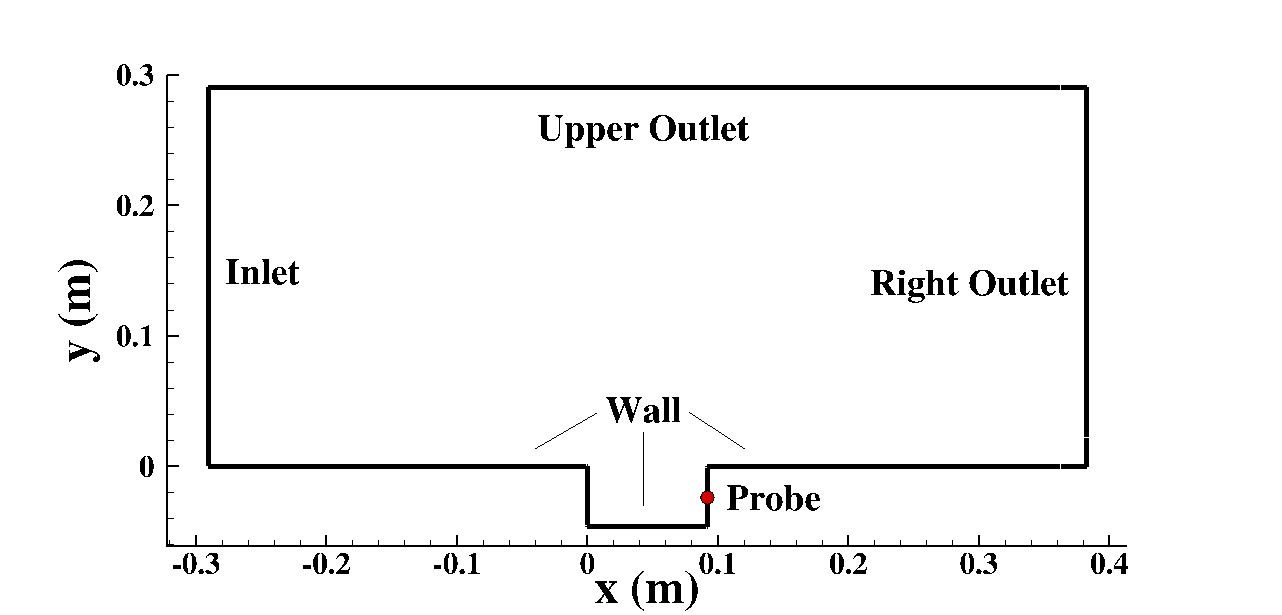
\includegraphics[width=0.9\linewidth]{Chapters/HPROMResults/Images/cavity/geom.png}
    \caption{\label{fig:cavityGeom}Cavity flow domain.}
\end{figure}

The working fluid is air, modeled as a calorically-perfect gas with the properties given in Table~\ref{tab:airProps}. Transport and thermodynamic properties are computed using the simplified analytical forms described in Section~\ref{subsec:gasModels}. The free-stream velocity is 208.7816 m/s in the +$x$-direction, the pressure is 25 Pa, and the temperature is 300 K. The resulting Mach number of this flow regime is approximately 0.6, and the Reynolds number based on the cavity length is approximately 6,500.

\begin{table}
	\centering
	\begin{tabular}{ lllll }
	\toprule
	MW (g/mol) & $c_p$ (kJ/kg-K) & $\mu$ (kg/m-s) & Pr & Sc   \\
	\midrule
	28.9604 & 1004.84 & 8.46e-7 & 0.72 & 0.62 \\
	\bottomrule
	\end{tabular}
	\caption{\label{tab:airProps}CPG properties of air for cavity flow case.}
\end{table}

The FOM is initialized with free stream conditions outside the cavity, and the inside of the cavity is initialized with free stream pressure and temperature, and zero velocity. The physical time step for the FOM simulation is $\dtFOM = 1 \;\mu$s. Initial transients are allowed to dissipate and statistically-steady flow is established over 100 ms. After this point, the simulation is continued for 10 ms, during which the state is saved to disk at every physical time step, resulting in 10,001 snapshots (including $\stateVec\left(\timeVar = 100 \; \text{ms}\right)$). All PROM simulations are restarted from $\timeVar = 100 \; \text{ms}$. Several instantaneous flow field examples are shown in Figs.~\ref{fig:cavityPressExample}--\ref{fig:cavityVExampleZoom}. Particular attention is drawn to the oscillatory pressure field displayed in Fig.~\ref{fig:cavityPressExample}: this emission of pressure waves from the trailing edge of the cavity is the result of the shear layer (originating from leading edge) impinging on the trailing edge. The shear layer rollup (implied by the $y$-velocity field in Fig.~\ref{fig:cavityVExampleZoom}) due to the Helmholtz instability and the pressure perturbation that travels upstream results in several resonant tones. Pressure measurements at the aft wall over the 10 ms data collection period is shown in Fig.~\ref{fig:cavityFOMProbe}.

\begin{figure}
	\centering
	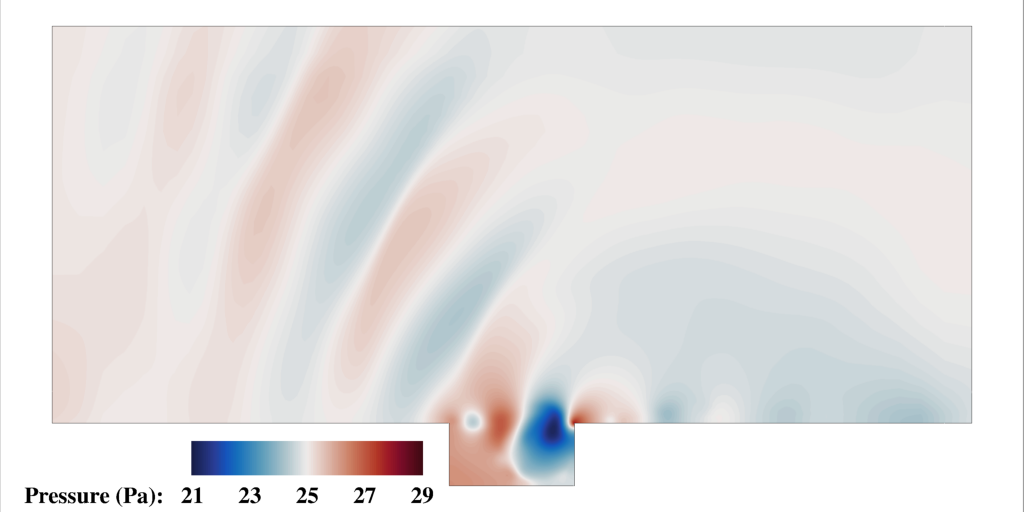
\includegraphics[width=0.9\linewidth,trim={0.5em 0.5em 0.5em 0.5em},clip]{Chapters/HPROMResults/Images/cavity/pressure_example_full.png}
	\caption{\label{fig:cavityPressExample}Cavity pressure field at $\timeVar =$ 104 ms.}
\end{figure}

\begin{figure}
	\begin{minipage}{0.48\linewidth}
		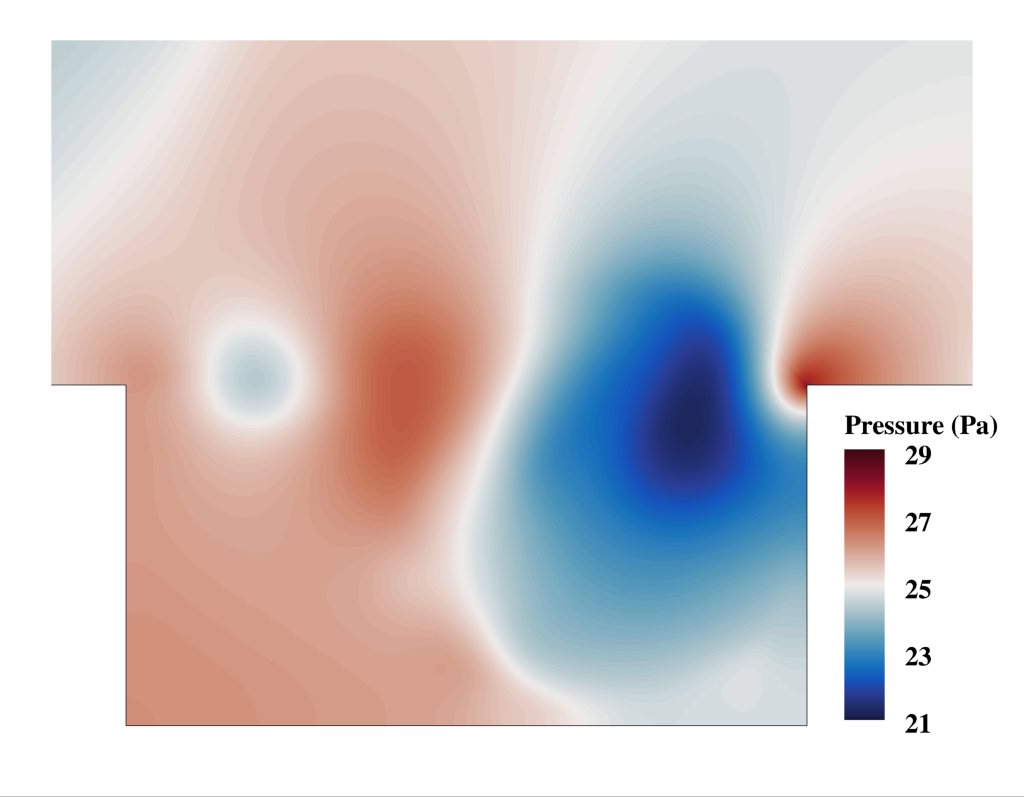
\includegraphics[width=0.99\linewidth,trim={0.5em 0.5em 0.5em 0.5em},clip]{Chapters/HPROMResults/Images/cavity/pressure_example_zoom.png}
		\caption{\label{fig:cavityPressExampleZoom}Cavity pressure field at $\timeVar =$ 104 ms, zoomed view.}
	\end{minipage} \hspace{0.5em}
	\begin{minipage}{0.48\linewidth}
		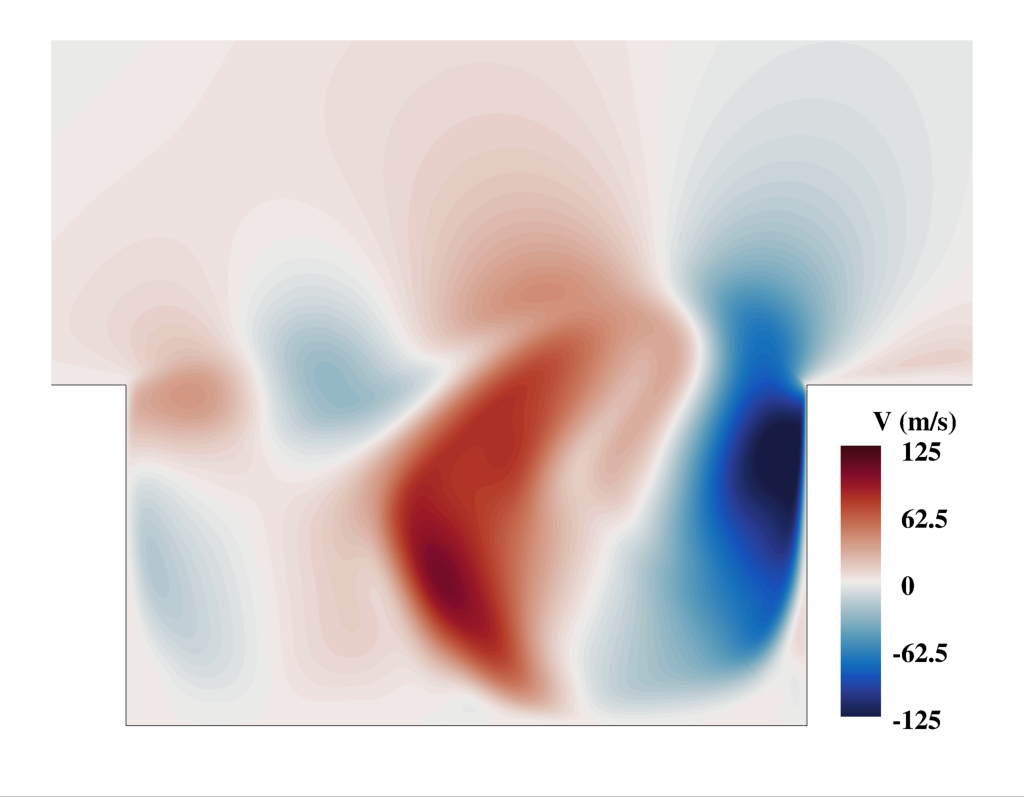
\includegraphics[width=0.99\linewidth,trim={0.5em 0.5em 0.5em 0.5em},clip]{Chapters/HPROMResults/Images/cavity/y_vel_example_zoom.png}
		\caption{\label{fig:cavityVExampleZoom}Cavity $y$-velocity field at $\timeVar =$ 104 ms, zoomed view.}
	\end{minipage}
\end{figure}

For this flow regime and cavity geometry, the formula of Rossiter~\cite{Rossiter1964} (with $\alpha = 0.25$, $\kappa = 0.57$) predicts the first three acoustic modes to be $f = \{725.2, \; 1,692.1, \; 2,659.1\}$ Hz. As a rough confirmation of model suitability, 100 ms ($\timeVar \in [100, \; 200]$ ms) of pressure data are collected from the aft wall point monitor. The signal is filtered using a low-pass fifth-order Butterworth filter with a critical frequency of 20 kHz, and the power spectral density is computed by Welch's method with a window of 25 ms and 75\% window overlap. The resulting sound pressure level is plotted in Fig.~\ref{fig:rossiterModeProof}, where the first three predicted Rossiter frequencies are marked in red. Although slightly overpredicting the first mode and underpredicting the third mode, this is a reasonable match in comparing an empirical fit model and a two-dimensional numerical simulation.

\begin{figure}
	\begin{minipage}{0.48\linewidth}
		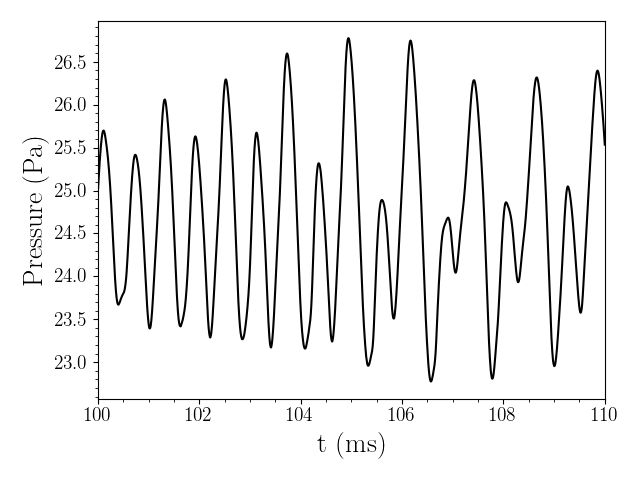
\includegraphics[width=0.99\linewidth,trim={0.5em 0.5em 0.5em 0.5em},clip]{Chapters/HPROMResults/Images/cavity/pressure_probe_fom_10ms.png}
		\caption{\label{fig:cavityFOMProbe}Pressure probe measurements from aft wall ($\timeVar \in [100, \; 110]$ ms).}
	\end{minipage} \hspace{0.5em}
	\begin{minipage}{0.48\linewidth}
		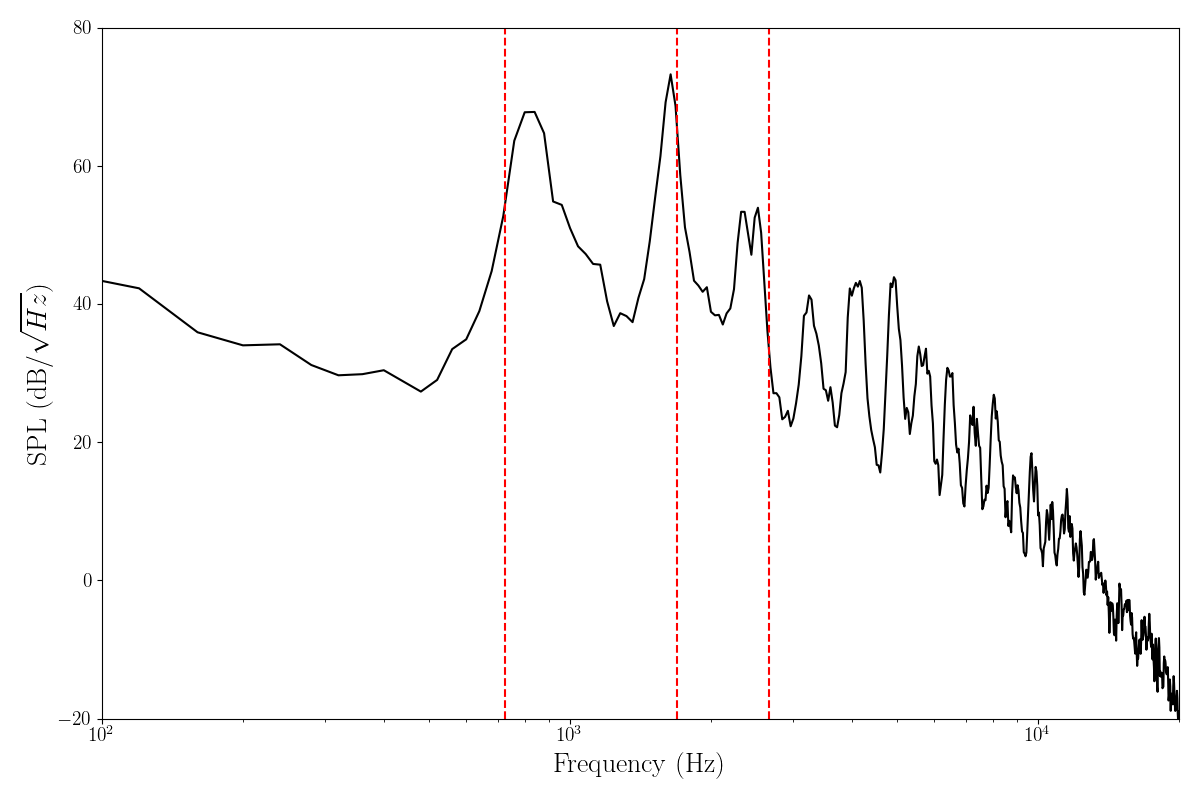
\includegraphics[width=0.99\linewidth,trim={0.5em 0.5em 0.5em 0.5em},clip]{Chapters/HPROMResults/Images/cavity/psd_fom_100ms.png}
		\caption{\label{fig:rossiterModeProof}Sound pressure level of aft wall pressure signal ($\timeVar \in [100, \; 200]$ ms). The first three Rossiter frequencies are marked in red.}
	\end{minipage}
\end{figure}

The POD trial bases are computed from the 10,001 snapshots of the conservative and primitive variables. The POD residual energy decay is displayed in Fig.~\ref{fig:cavityPODEnergy}. Achieving 1\%, 0.1\%, and 0.01\% of the conservative state POD residual energy requires 20, 73, and 155 modes respectively. For the primitive state, this increases to 26, 92, and 180 modes respectively. Although this is a fairly simple problem without any reaction phenomena, this slow POD residual energy decay exhibits how traveling waves and large fluctuations in the unsteady flow field can require a large number of trial bases to approximate accurately. Indeed, the primitive and conservative variable projection error plots in Fig.~\ref{fig:cavityProjErr} indicate that over 125 modes are required to decrease the projection error of velocity and momentum magnitudes below 0.1\% relative error.

\begin{figure}
	\centering
	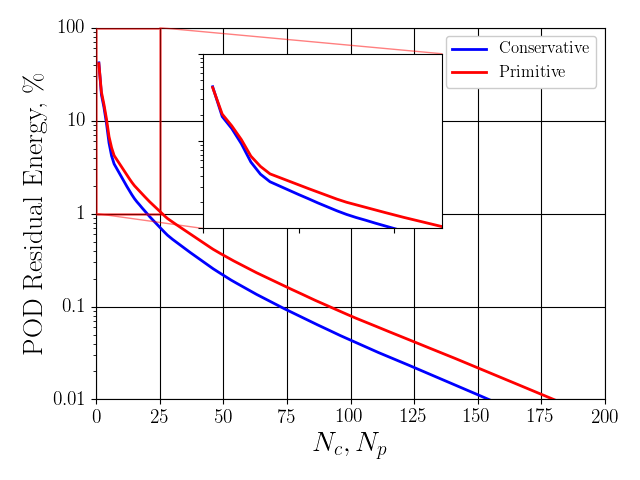
\includegraphics[width=0.75\linewidth]{Chapters/HPROMResults/Images/cavity/cavity_pod_energy_10ms.png}
	\caption{\label{fig:cavityPODEnergy}Cavity POD residual energy for conservative and primitive state datasets.}
\end{figure}

\begin{figure}
	\begin{minipage}{0.49\linewidth}
		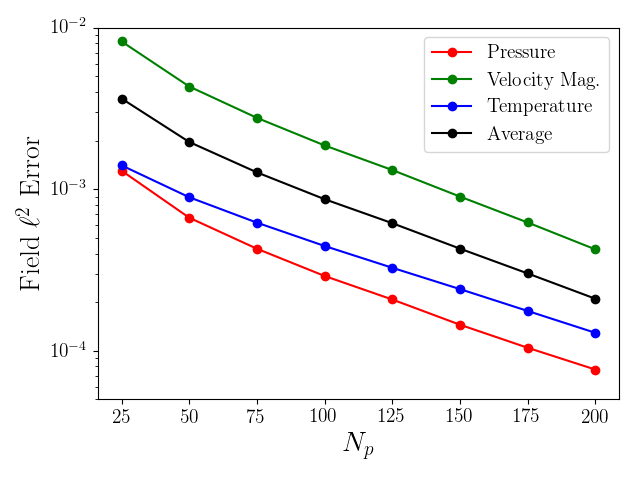
\includegraphics[width=0.99\linewidth,trim={0.5em 0.5em 0.5em 0.5em},clip]{Chapters/HPROMResults/Images/cavity/projection_error_primitive.png}
		\subcaption{Primitive variables}
	\end{minipage}
	\begin{minipage}{0.49\linewidth}
		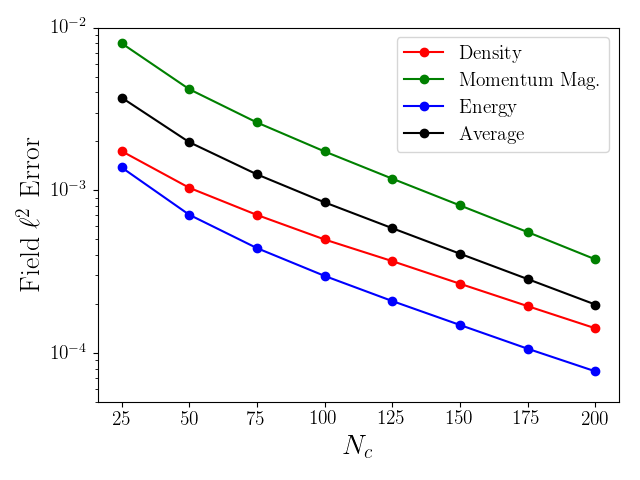
\includegraphics[width=0.99\linewidth,trim={0.5em 0.5em 0.5em 0.5em},clip]{Chapters/HPROMResults/Images/cavity/projection_error_conservative.png}
		\subcaption{Conservative variables}
	\end{minipage}
	\caption{\label{fig:cavityProjErr}Cavity time-average POD projection error.}
\end{figure}

\subsection{Unsampled PROMs}

The performance of unsampled Galerkin, LSPG, and MP-LSVT PROMs is examined first. As mentioned previously, the application of projection-based ROMs alone does not result in computational cost reduction, but still serves as a good performance baseline. If the unsampled PROM performs poorly, the hyper-reduced PROM can hardly be expected to perform well.

A trial basis dimension study and time step size study is conducted. The trial basis dimension $\numConsModes$/$\numPrimModes$ is swept from 25 modes to 200 modes at 25-mode intervals. Four time step sizes are examined: $\Delta \timeVar \in \{ 1, \; 2.5, \; 5, \; 10 \} \; \mu \text{s}$, or 1, 2.5, 5, and 10 times that of the FOM simulation. As has been documented by previous work~\cite{Carlberg2017,Huang2022,Wentland2021}, increasing the PROM time step often achieves computational speedup with negligible increase in error relative to PROMs for which $\dt = \dtFOM$, up to a point. Average error results for each evaluated time step are displayed in Fig.~\ref{fig:cavityUnsampledROMErrVsModes}. Several indicative pressure probe measurements are displayed in Fig.~\ref{fig:cavityUnsampledROMProbes}.

\begin{figure}
	\begin{minipage}{0.49\linewidth}
		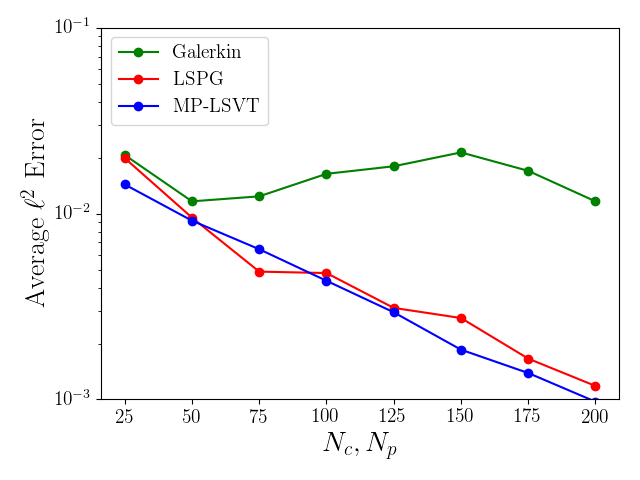
\includegraphics[width=0.99\linewidth]{Chapters/HPROMResults/Images/cavity/unsampled/unsampled_dt1e-6_Average_errorRaw.png}
		\subcaption{$\dt = \dtFOM$}
	\end{minipage}
	\begin{minipage}{0.49\linewidth}
		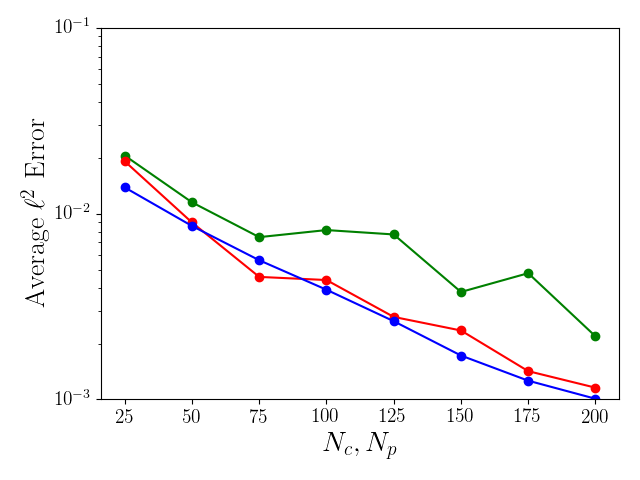
\includegraphics[width=0.99\linewidth]{Chapters/HPROMResults/Images/cavity/unsampled/unsampled_dt2p5e-6_Average_errorRaw.png}
		\subcaption{$\dt = 2.5 \times \dtFOM$}
	\end{minipage}

	\begin{minipage}{0.49\linewidth}
		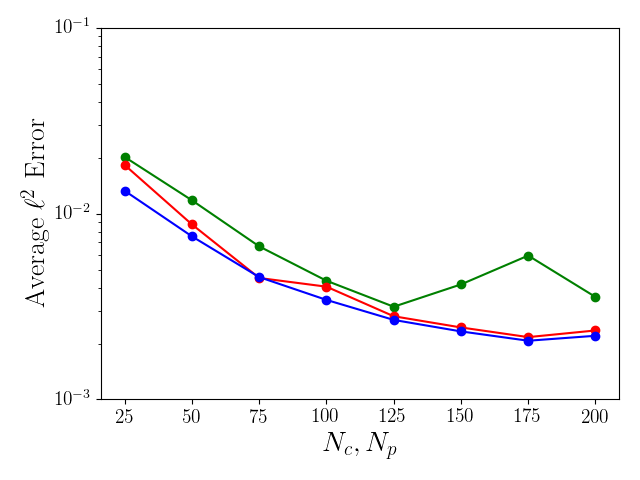
\includegraphics[width=0.99\linewidth]{Chapters/HPROMResults/Images/cavity/unsampled/unsampled_dt5e-6_Average_errorRaw.png}
		\subcaption{\label{fig:cavityUnsampledROMErrVsModesDt5en6}$\dt = 5 \times \dtFOM$}
	\end{minipage}
	\begin{minipage}{0.49\linewidth}
		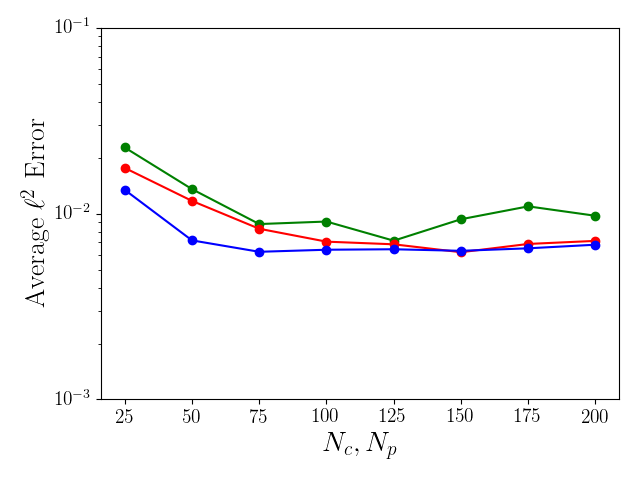
\includegraphics[width=0.99\linewidth]{Chapters/HPROMResults/Images/cavity/unsampled/unsampled_dt1e-5_Average_errorRaw.png}
		\subcaption{$\dt = 10 \times \dtFOM$}
	\end{minipage}
	\caption{\label{fig:cavityUnsampledROMErrVsModes}Cavity unsampled PROM time-average error, various $\dt$.}
\end{figure}

\begin{figure}
	\begin{minipage}{0.49\linewidth}
		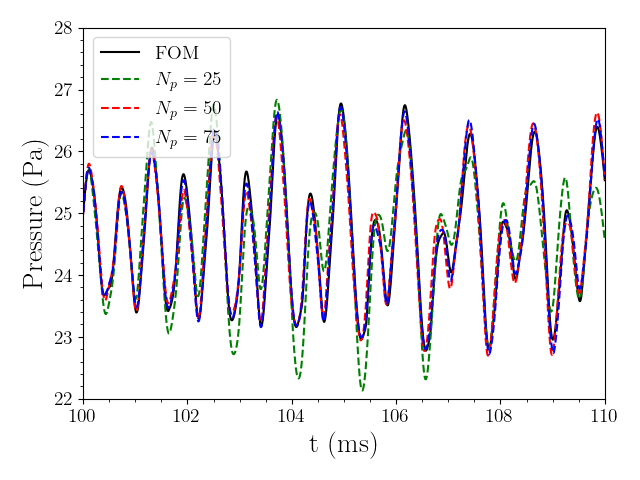
\includegraphics[width=0.99\linewidth]{Chapters/HPROMResults/Images/cavity/unsampled/pressure_probe_unsampled_modes.png}
		\subcaption{\label{fig:cavityUnsampledROMProbesModes}MP-LSVT method, various $\numPrimModes$.}
	\end{minipage}
	\begin{minipage}{0.49\linewidth}
		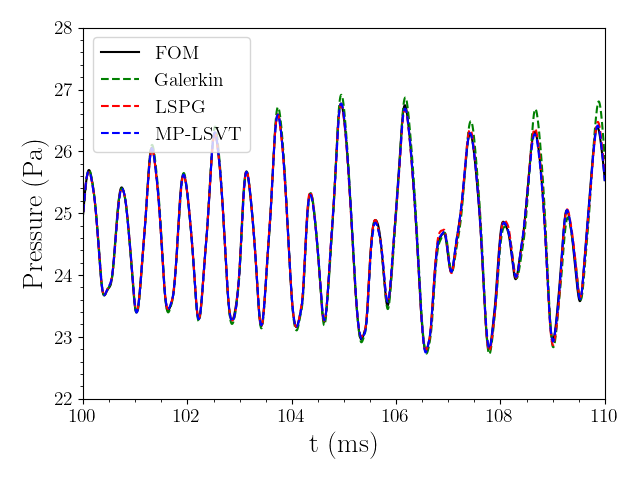
\includegraphics[width=0.99\linewidth]{Chapters/HPROMResults/Images/cavity/unsampled/pressure_probe_unsampled_methods.png}
		\subcaption{\label{fig:cavityUnsampledROMProbesMethods}$\numConsModes,\numPrimModes$ = 150, various methods.}
	\end{minipage}
	\caption{\label{fig:cavityUnsampledROMProbes}Cavity unsampled PROM probe measurements, $\dt = 5 \times \dtFOM$.}
\end{figure}

Unremarkably, the LSPG and MP-LSVT PROMs outperform the Galerkin PROMs at all mode counts and time steps. Further, the LSPG and MP-LSVT PROMs generally exhibit non-increasing accuracy with trial basis enrichment, while error often \textit{increases} with trial basis enrichment for the Galerkin PROMs. For all time steps and trial basis dimensions evaluated, the LSPG and MP-LSVT PROMs perform similarly. This is not unexpected, as this is a non-reacting simulation which does not involve stiff source terms, extremely disparate spatio-temporal scales, or poor conditioning from which traditional LSPG PROMs might suffer. As mentioned previously, increasing the PROM time step may result in ``free'' computational cost savings. Indeed, increasing the PROM time step to $\dt = 2.5 \times \dtFOM$ generates virtually no error increase for the LSPG and MP-LSVT PROMs, and even improves the performance of the Galerkin PROMs. However, at higher time step sizes, the accuracy of all PROMs for roughly $\numConsModes$, $\numPrimModes > 50$ deteriorate drastically. In fact, for $\dt = 10 \times \dtFOM$, accuracy improvement via trial basis enrichment saturates at $\numConsModes$, $\numPrimModes = 50$, never dropping below 0.5\%.

The pressure probe monitors in Fig.~\ref{fig:cavityUnsampledROMProbes} display largely unsurprising results. As seen in Fig~\ref{fig:cavityUnsampledROMProbesModes}, a very low trial basis dimension ($\numPrimModes = 25$), the solution quickly deviates and fails to reconstruct the FOM data faithfully. Large over- and under-shoot in the unsteady pressure signal are observed, and by the end of the simulation period the signal has devolved into small, unorganized fluctuations. Increasing the resolution to $\numPrimModes = 50$ improves the signal reconstruction, although small under- and over-shoot is observed by $\timeVar = 103$ ms. This small discrepancy is only marginally improved by increasing the trial basis dimension to $\numPrimModes = 75$, in agreement with the converging average error shown in Fig.~\ref{fig:cavityUnsampledROMErrVsModesDt5en6}.

\begin{figure}
    \centering
    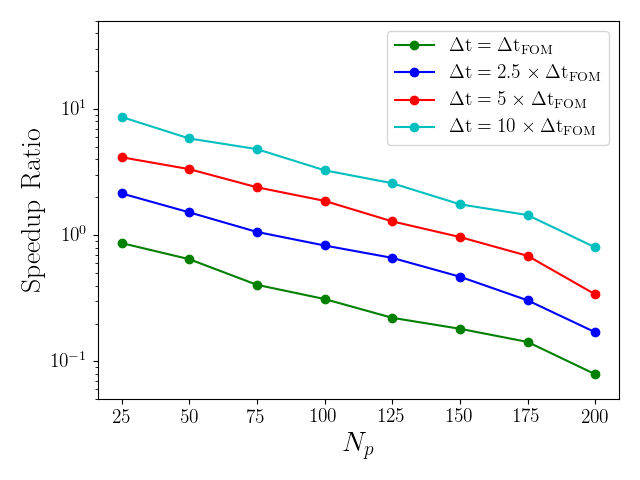
\includegraphics[width=0.7\linewidth]{Chapters/HPROMResults/Images/cavity/unsampled/unsampled_modeStudy_time_calcAndMPI.png}
    \caption{\label{fig:cavityUnsampledCost}MP-LSVT unsampled PROM computational cost, relative to FOM cost, various $\dt$.}
\end{figure}

The computational cost of the unsampled MP-LSVT PROMs is now examined. Results are nearly identical for equivalent Galerkin and LSPG PROMS. As discussed previously, projection-based ROMs \textit{alone} should not produce any significant computational cost savings, and in fact should increase cost due to lifting the state to the full-dimension and projecting the non-liner function onto the test space. Figure~\ref{fig:cavityUnsampledCost} quantifies just how much this change affects the run-time of the unsampled PROM. Note that using the same time step size as that of the FOM, the unsampled PROM is always more expensive than the FOM (below 1 on the $y$-axis) no matter the trial basis dimension. This highlights the necessity of hyper-reduction: projection-based order reduction of the governing system alone, even for extremely low trial/test basis dimensions, does not improve PROM computational cost. For $\dt = 2.5 \times \dtFOM$, the unsampled PROM only achieves speedup for $\numPrimModes < 100$. This trend continues to improve the speedup for $\dt = 5 \times \dtFOM, \; 10 \times \dtFOM$, though prior results showed that PROM accuracy quickly deteriorates at high time steps. For $\numPrimModes = 100$ and $\dt = 10 \times \dtFOM$, the unsampled PROM is only capable of achieving three times speedup, which is hardly impressive given that these results only reconstruct the training period. To realize significant cost savings, hyper-reduction must be applied.

\subsection{Hyper-reduced PROMs}
%
For the sake of brevity, only MP-LSVT HPROMs are examined. As will be seen in Section~\ref{sec:cvrc}, Galerkin and LSPG PROMs appear unsuitable for practical reacting flows, and will not be discussed thereafter. All results presented in this section utilize a trial basis dimension of $\numPrimModes = 150$. All gappy POD regressor bases are constructed from POD modes of the conservative field dataset, i.e., $\deimBasis = \consTrial \inRTwo{\numDOF}{\numResModes}$, as detailed in Section~\ref{subsec:stateApproxDEIM}

\begin{figure}
	\begin{minipage}{0.49\linewidth}
		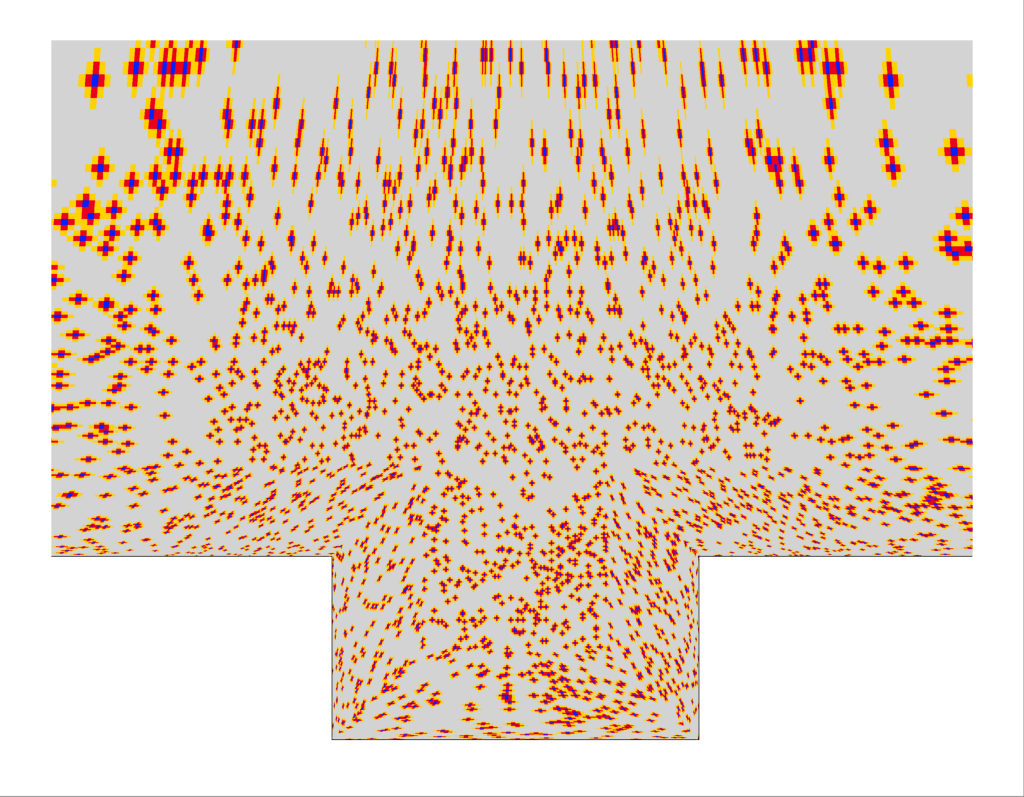
\includegraphics[width=0.99\linewidth,trim={0.5em 0.5em 0.5em 0.5em},clip]{Chapters/HPROMResults/Images/cavity/deim/iBlank_random_zoom.png}
		\subcaption{Random}
	\end{minipage}
	\begin{minipage}{0.49\linewidth}
		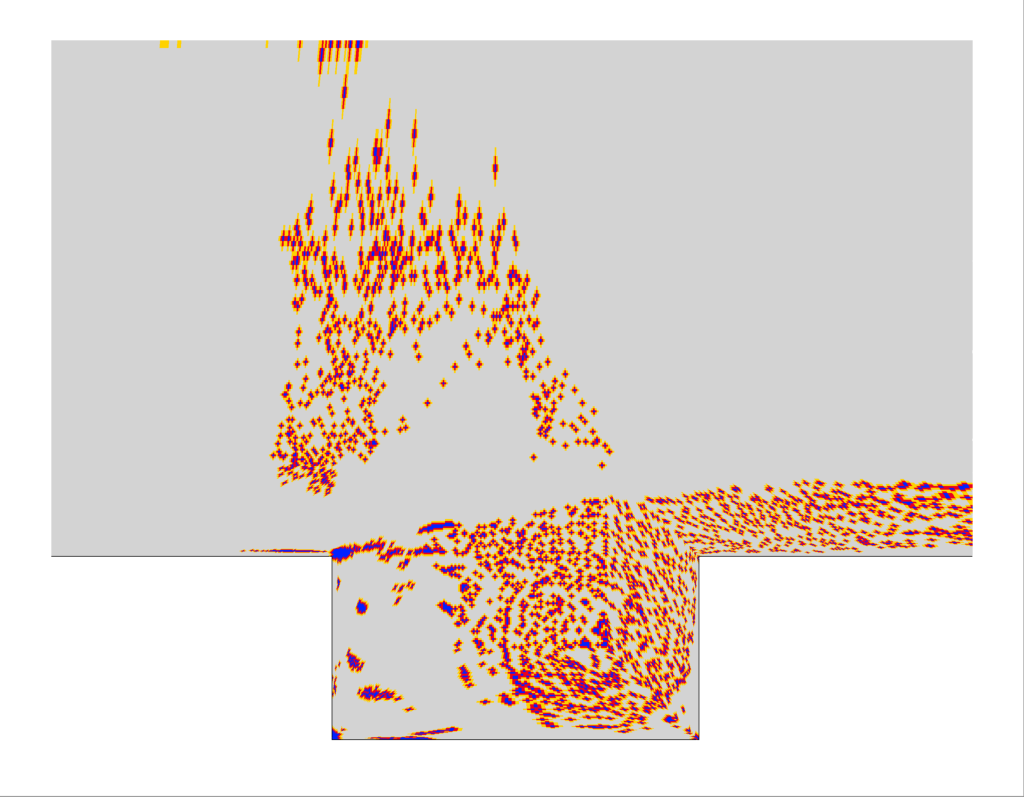
\includegraphics[width=0.99\linewidth,trim={0.5em 0.5em 0.5em 0.5em},clip]{Chapters/HPROMResults/Images/cavity/deim/iBlank_eigenvec_zoom.png}
		\subcaption{Eigenvector}
	\end{minipage}

	\begin{minipage}{0.49\linewidth}
		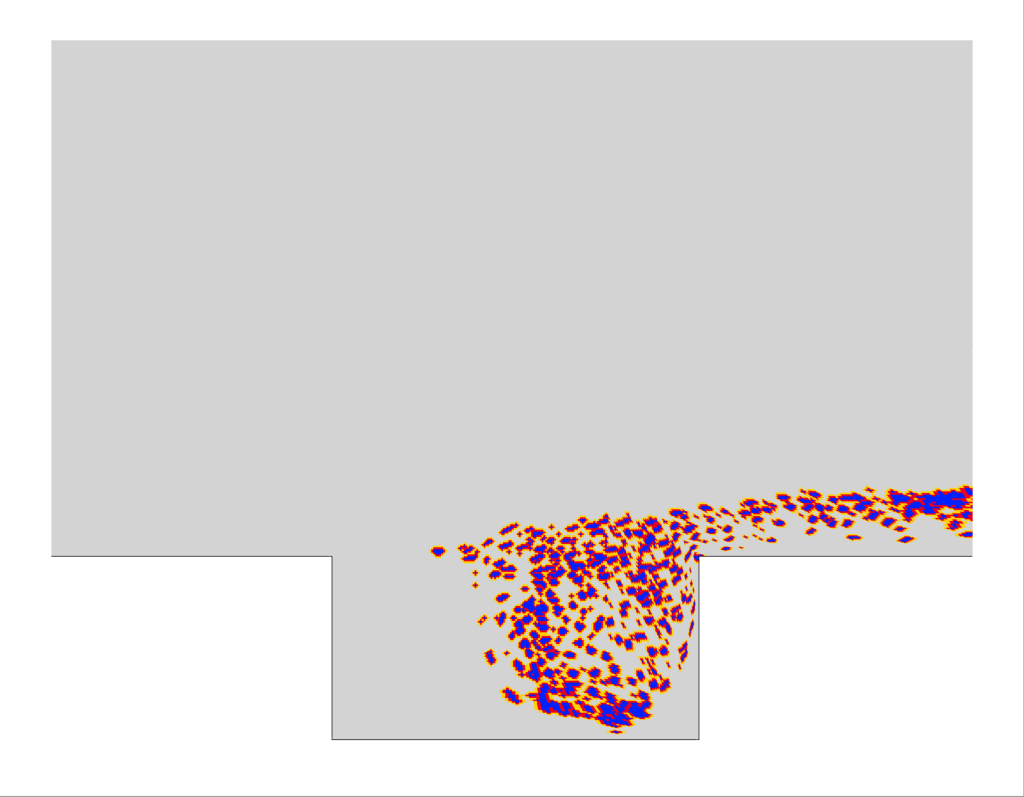
\includegraphics[width=0.99\linewidth,trim={0.5em 0.5em 0.5em 0.5em},clip]{Chapters/HPROMResults/Images/cavity/deim/iBlank_greedy_carlberg_zoom.png}
		\subcaption{GNAT V1}
	\end{minipage}
	\begin{minipage}{0.49\linewidth}
		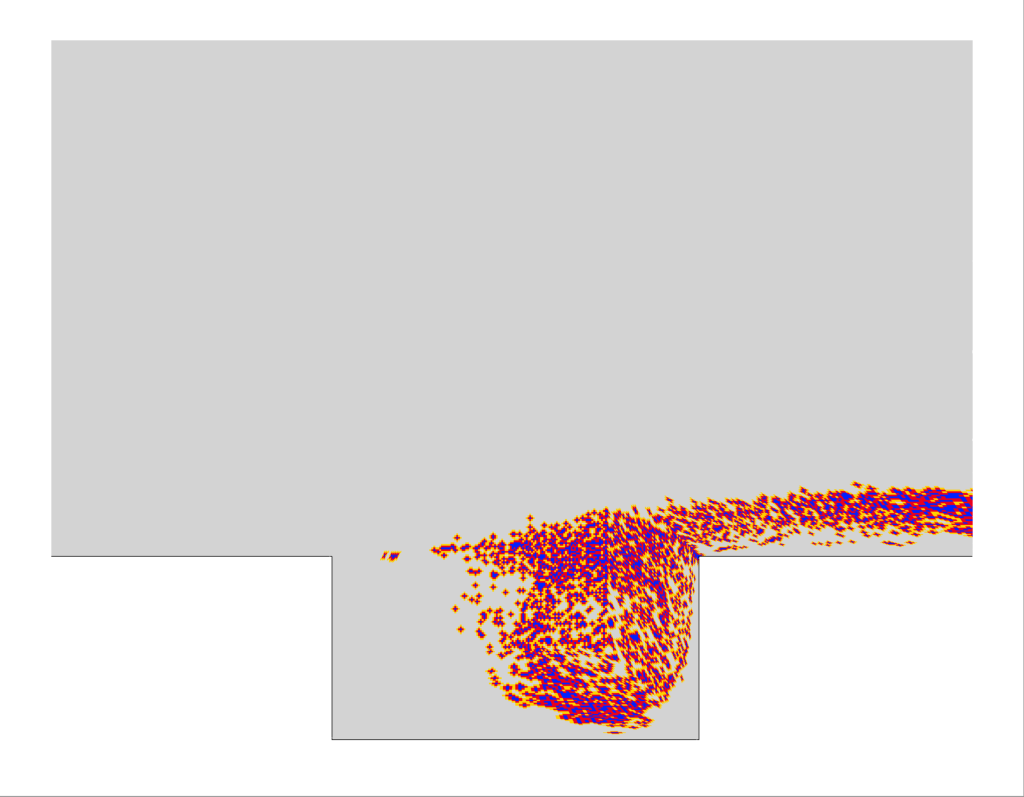
\includegraphics[width=0.99\linewidth,trim={0.5em 0.5em 0.5em 0.5em},clip]{Chapters/HPROMResults/Images/cavity/deim/iBlank_greedy_ben_zoom.png}
		\subcaption{GNAT V2}
	\end{minipage}
	\caption{\label{fig:cavityiBlank}Cavity sample mesh examples, $\numResModes= 250$, $\numSamps = 2.5\% \times \numDOF$.}
\end{figure}

\begin{table}
	\centering
	\begin{tabular}{ llllllllll }
	\toprule
	Sampling Rate (\%) & 0.5 & 0.75 & 1 & 1.75 & 2.5 & 3.75 & 5.0 & 7.5 & 10 \\
	\midrule
	Cores & 2 & 2 & 2 & 2 & 3 & 5 & 6 & 9 & 13 \\
	Cells/core (approx.) & 312 & 469 & 625 & 1,093 & 1,042 & 938 & 1,042 & 1,042 & 962 \\
	\bottomrule
	\end{tabular}
	\caption{\label{tab:cavitySampProcs}Partitioning for cavity HPROM sample meshes.}
\end{table}

The accuracy and computational performance of the HPROMs is examined for sampling rates of $\numSamps \in \{0.5, \; 0.75, \; 1.0, \; 1.75, \; 2.5, \; 3.75, \; 5.0, \; 7.5, \; 10\}\% \times \numDOF$, and gappy POD regressor dimensions of $\numResModes \in \{150, \; 200, \; 250, \; 300\}$. Views of indicative sample meshes constructed using the four sampling algorithms detailed in Section~\ref{subsec:sampAlgos} are shown in Fig.~\ref{fig:cavityiBlank}. As in Section~\ref{sec:sampleMesh}, blue cells indicate directly-sampled cells, red cells indicate flux cells, and yellow cells indicate gradient/vertex cells. The three greedy sampling algorithms generate sample meshes which are quite similar in some ways: the vast majority of sampled cells are located in the shear layer originating from the cavity leading edge and meandering downstream, as well as in the strong recirculation region in the downstream half of the cavity. The most glaring difference appears to be that the eigenvector-based algorithm also selects a number of points in the free-stream flow. Note that this region, although dominated by the free-stream conditions, experiences strong pressure oscillations emitted from the cavity trailing edge. Interestingly, the GNAT V1 algorithm selects sample cells in extremely tight clusters, while GNAT V2 generates a relatively more diffuse sample mesh, and the eigenvector-based algorithm's sample mesh is even more diffuse. Further, the eigenvector-based sampling selects a significant number of points on the leading edge of the cavity and in the upstream half of the cavity. It will be shown shortly how apparently minor discrepancies can have a drastic effect on HPROM performance. For all online HPROM results, each sample mesh is partitioned for parallel computations according to the sampling rate, as given in Table~\ref{tab:cavitySampProcs}, regardless of the sampling algorithm utilized. The number of cores is altered for each sampling rate to ensure approximately equal load balancing, amounting to roughly 1,000 cells per core. Note that this is impossible for $\numSamps \le 1\% \times \numDOF$, and two cores are used for such cases.

\begin{figure}
	\begin{minipage}{0.46\linewidth}
		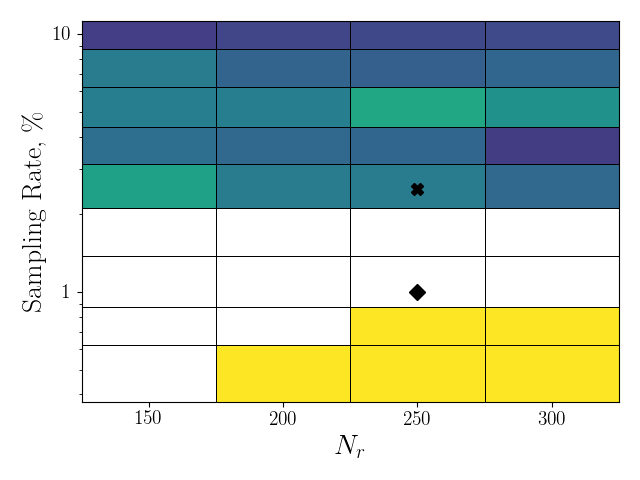
\includegraphics[width=0.99\linewidth]{Chapters/HPROMResults/Images/cavity/deim/err_contour_random_dt5e-6.png}
		\subcaption{Random}
	\end{minipage}
	\begin{minipage}{0.53\linewidth}
		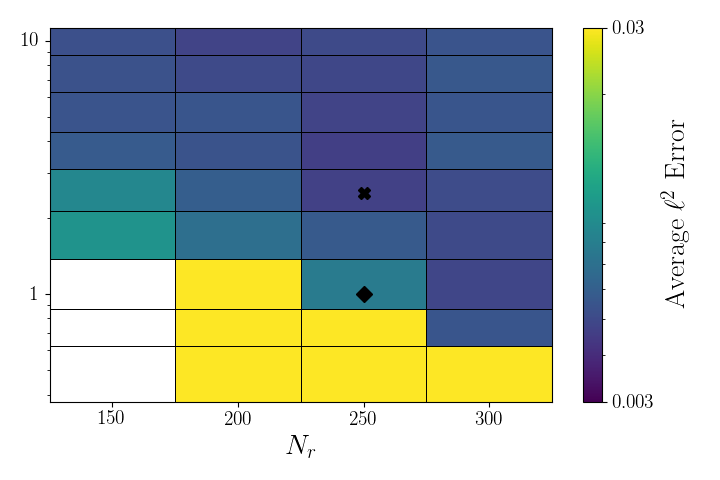
\includegraphics[width=0.99\linewidth]{Chapters/HPROMResults/Images/cavity/deim/err_contour_eigenvec_dt5e-6.png}
		\subcaption{Eigenvector}
	\end{minipage}

	\begin{minipage}{0.46\linewidth}
		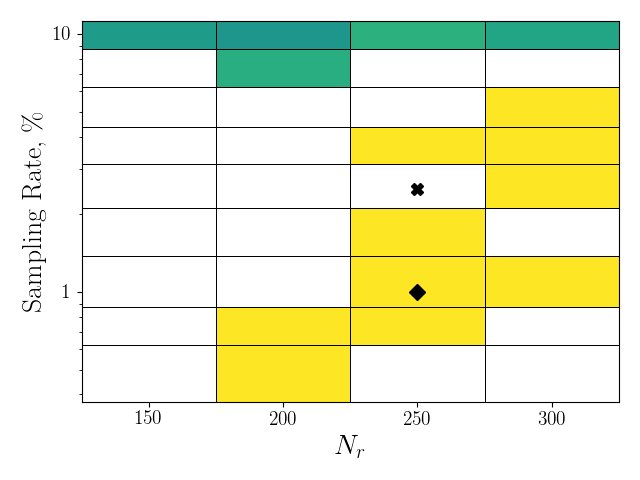
\includegraphics[width=0.99\linewidth]{Chapters/HPROMResults/Images/cavity/deim/err_contour_gnat1_dt5e-6.png}
		\subcaption{GNAT, V1}
	\end{minipage}
	\begin{minipage}{0.53\linewidth}
		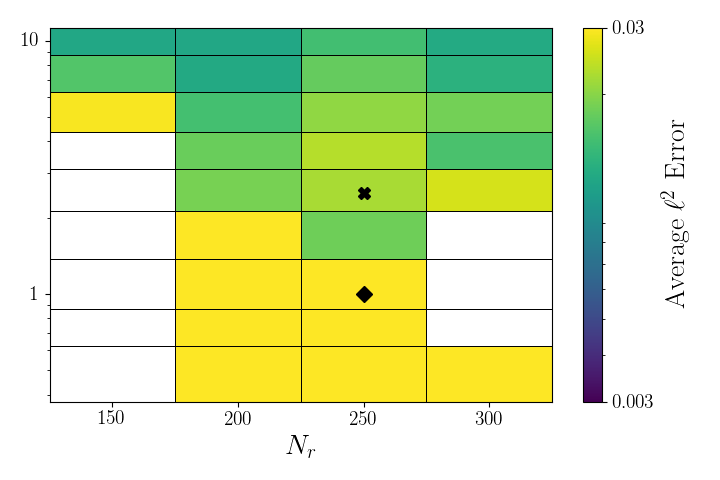
\includegraphics[width=0.99\linewidth]{Chapters/HPROMResults/Images/cavity/deim/err_contour_gnat2_dt5e-6.png}
		\subcaption{GNAT, V2}
	\end{minipage}
	\caption{\label{fig:cavitySampledROMErrContour}Cavity HPROM time-average error contours with respect to gappy POD regressor dimension and sampling rate, $\dt = 5 \times \dtFOM$, various sampling algorithms.}
\end{figure}

The accuracy of the online HPROMs on sample meshes generated by each sampling algorithm stand in stark contrast. Time-average $\ell^2$ error contour plots for $\dt = 5 \times \dtFOM$ are given in Fig.~\ref{fig:cavitySampledROMErrContour},comparing accuracy at each combination of sampling rate $\numSamps$ and gappy POD regressor basis dimension $\numResModes$. White squares indicate simulations which exploded. Across all sampling algorithms, note the unsurprising result that increasing $\numSamps$ and $\numResModes$ tends to improve HPROM performance. However, it is quite plain that eigenvector-based sampling consistently generates more stable and accurate HPROMs than any other sampling algorithm, only failing at extremely low sampling rates. Interestingly, random sampling tends to outperform both GNAT sampling algorithms, though it only produces stable simulations for $\numSamps > 2.5\% \times \numDOF$. In fact, GNAT V1 produces consistently stable simulations only for $\numSamps = 10\% \times \numDOF$, and even those are highly inaccurate. The GNAT V2 algorithm is capable of producing stable simulations at lower sampling rates, but also incurs relatively high error in the solution.

\begin{figure}
	\begin{minipage}{0.49\linewidth}
		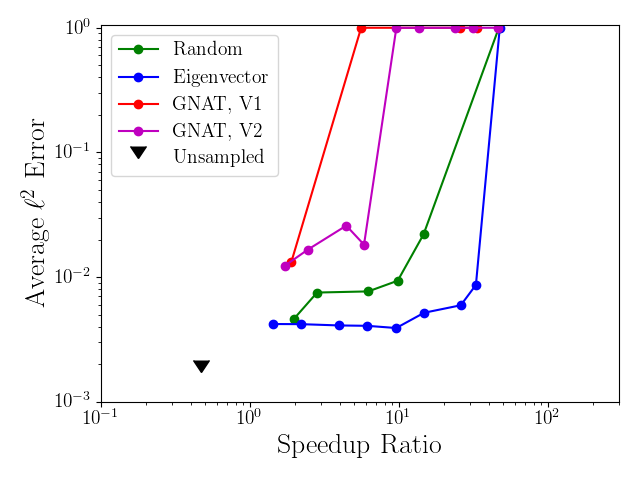
\includegraphics[width=0.99\linewidth]{Chapters/HPROMResults/Images/cavity/deim/sampled_dt2p5e-6_Average_errorRaw_pareto.png}
		\subcaption{$\dt = 2.5 \times \dtFOM$}
	\end{minipage}
	\begin{minipage}{0.49\linewidth}
		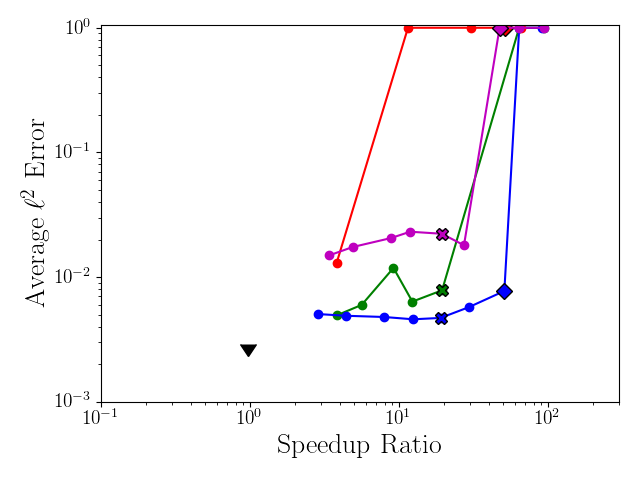
\includegraphics[width=0.99\linewidth]{Chapters/HPROMResults/Images/cavity/deim/sampled_dt5e-6_Average_errorRaw_pareto.png}
		\subcaption{$\dt = 5 \times \dtFOM$}
	\end{minipage}
	% \begin{minipage}{0.49\linewidth}
	% 	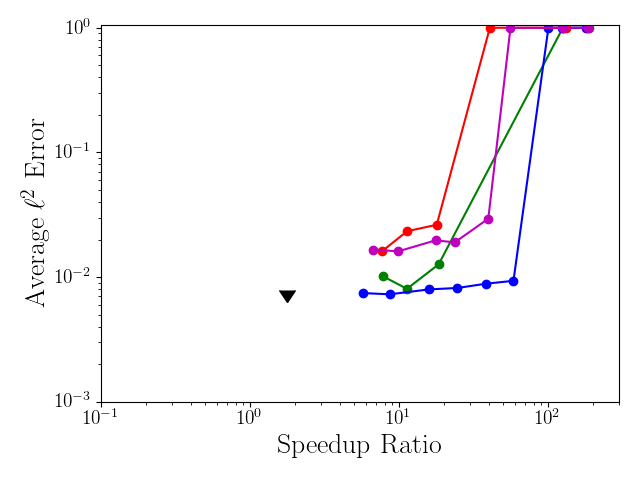
\includegraphics[width=0.99\linewidth]{Chapters/HPROMResults/Images/cavity/deim/sampled_dt1e-5_Average_errorRaw_pareto.png}
	% 	\subcaption{$\dt = 10 \times \dtFOM$}
	% \end{minipage}
	\caption{\label{fig:cavitySampledROMErrVsTime}Cavity HPROM error vs. CPU-time speedup, $\numPrimModes = 150$, $\numResModes = 250$, various $\dt$.}
\end{figure}

Of course, computational cost savings is the prime objective of hyper-reduction, and an accurate HPROM does not guarantee a fast HPROM. As one might expect, increasing $\numSamps$ and $\numResModes$ increases HPROM computational cost, as will be explored more thoroughly in Section~\ref{sec:cvrc}. Figure~\ref{fig:cavitySampledROMErrVsTime} displays the time-average error with respect to the speedup ratio at each sampling rates for all sampling algorithms. The eigenvector-based sampling enables stable, accurate HPROMs which are able to achieve over 200 times computational cost savings, while the equivalent unsampled PROMs are either equally or more expensive than the FOM. Similarly, random sampling is capable of producing accurate ($<1\%$ error), though only at higher sampling rates and achieving relatively lower speedup ratios. The GNAT sampling algorithms generally fail to produce meaningful cost savings without incurring instability or high error.

\begin{figure}
	\begin{minipage}{0.49\linewidth}
		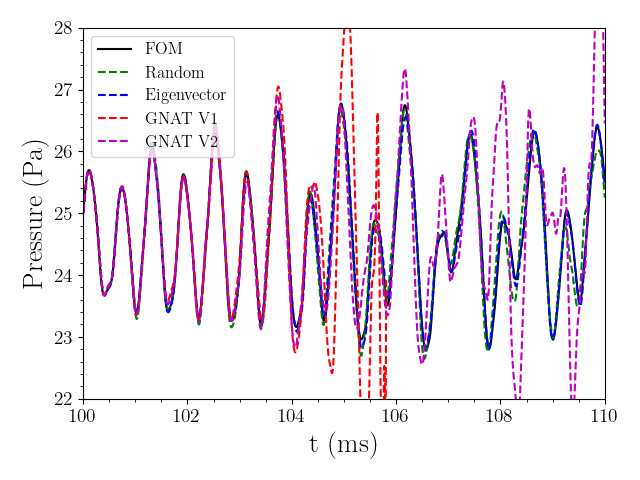
\includegraphics[width=0.99\linewidth]{Chapters/HPROMResults/Images/cavity/deim/pressure_probe_deim_2p5.png}
		\subcaption{\label{fig:cavitySampledROMProbe2p5}$\numSamps = 2.5\% \times \numDOF$}
	\end{minipage}
	\begin{minipage}{0.49\linewidth}
		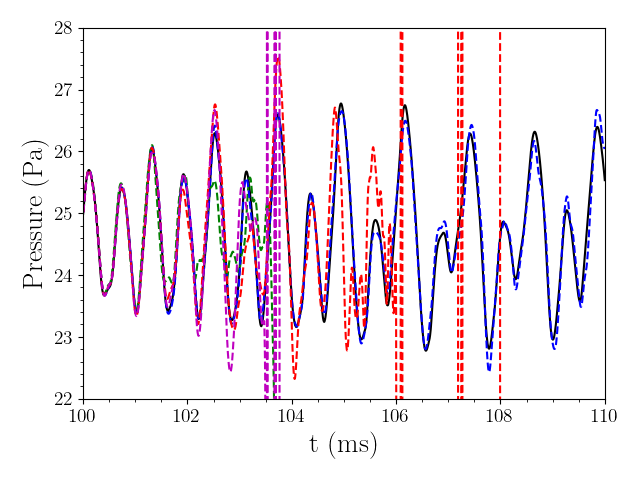
\includegraphics[width=0.99\linewidth]{Chapters/HPROMResults/Images/cavity/deim/pressure_probe_deim_1.png}
		\subcaption{\label{fig:cavitySampledROMProbe1p}$\numSamps = 1\% \times \numDOF$}
	\end{minipage}
	\caption{\label{fig:cavitySampledROMProbes}Cavity MP-LSVT HPROM probe measurements, $\numPrimModes = 150$, $\numResModes = 250$, $\dt = 5 \times \dtFOM$.}
\end{figure}

To better visualize these accuracy discrepancies, Fig.~\ref{fig:cavitySampledROMProbes} displays pressure probe monitors for each sampling algorithm for two different sampling rates. The corresponding average error for Fig.~\ref{fig:cavitySampledROMProbe2p5} are marked with an ``X'' in Figs.~\ref{fig:cavitySampledROMErrContour} and~\ref{fig:cavitySampledROMErrVsTime}, and those for Fig.~\ref{fig:cavitySampledROMProbe1p} are similarly marked by a diamond. In general, all sampling algorithms are able to produce stable and accurate PROMs for the simulation period $\timeVar \in [100, \; 102]$ ms. However, those HPROMs generated by the GNAT sampling algorithms quickly deviate from the FOM, exhibiting wild swings in the unsteady pressure signal. Although random sampling generates an unstable HPROM for $\numSamps = 1\% \times \numDOF$, it produces a fairly accurate simulation for $\numSamps = 2.5\% \times \numDOF$, only exhibiting minor under- and over-shoot towards the end of the simulation period. Eigenvector-based sampling produces accurate reconstruction of the unsteady pressure signal, particularly for $\numSamps = 2.5\% \times \numDOF$, though it does exhibit some discrepancies at later times for $\numSamps = 1\% \times \numDOF$.

Although the above results indicate that it is possible to achieve excellent computational cost savings with HPROMs, they also hint at the challenge of guaranteeing that they are accurate and robust. The drastic effects that the sample mesh and gappy POD regression have on HPROM performance invites more thorough exploration for larger, more challenging systems.
\section{Continuously-variable Resonance Chamber}\label{sec:cvrc}


% \subsection{High-amplitude Pressure Wave Reconstruction}
\section{Nine-element Combustor}\label{app:nineElemSupp}
\chapter{Supplementary Results}
\label{app:suppResults}

In the author's personal experience, there is often a certain opacity in the projection-based ROM literature on the subject of data preparation and robustness controls. In many cases this is simply due to the fact that many PROM studies deal with systems which are governed by a single state variable (Burgers' equation, Kuramoto--Sivashinsky equation), are governed by state variables that are naturally of similar magnitudes (shallow water equations, Euler equations for Sod shock tube), or are commonly non-dimensionalized in open-source or commercial solvers (incompressible Navier--Stokes). In such situations, the dimensionality of the state variables is either irrelevant or has little effect on the accuracy of state representations and the solution of the PROM equations. Sometimes, however, small but crucial details of data preparation or the PROM solution are left out as they are considered self-evident to the authors (as has been discovered anecdotally by this author and colleagues). To date, the work by Parish and Rizzi~\cite{Parish2022} provides the most explicit description and comprehensive study of ensuring a dimensionally-consistent POD formulation and PROM solution by careful choice of inner products. Although the focus of their work is the compressible Euler equations, they provides broadly-meaningful insights for dimensional dynamical systems.

All but one numerical experiment in this thesis deals with high-pressure, compressible reacting flows, which are characterized by both vastly disparate magnitudes in the system state and an inability to readily non-dimensionalize the governing equations. As such, careful data preparation and unsteady solution robustness controls are extremely important in enabling the stable and accurate solution of projection-based reduced-order models. Further, this thesis aims to be as transparent about every element of the PROM construction process to help enable successful PROMs for future researchers working with similarly-complex systems. Some of the key elements in this process are detailed the numerical experiments which follow.

All results shown in this chapter are unsampled MP-LSVT PROMs of the truncated CVRC case investigated in Section~\ref{sec:cvrc}. A time step of $\dt = 5 \times \dtFOM$ is used in all cases.
\section{Transient Flame}\label{app:transientFlameSupp}


To begin this section, two-dimensional transonic flow over an open cavity is examined. Flow over open cavities has been studied extensively due to its practical applications in aviation (e.g., bomb or landing gear bays) and the interesting acoustic phenomena it exhibits, particularly the resonant coupling of the cavity leading edge shear layer and acoustic feedback from the cavity trailing edge. Pioneering experimental work in the mid-1900's such as that by Roshko~\cite{Roshko1952}, Krishnamurty~\cite{Krishnamurty1955}, and Rossiter~\cite{Rossiter1964}, numerical modeling work such as that by Colonius \textit{et al.}~\cite{Colonius1999}, Rowley \textit{et al.}~\cite{Rowley2002}, and Larchev\^{e}que \textit{et al.}~\cite{Larcheveque2007}, and more recent experimental efforts such as those by Wagner\textit{et al.}~\cite{Wagner2015} and Casper \textit{et al.}~\cite{Casper2018} have investigated the effects of cavity dimensions, freestream flow regime, and turbulence on the behavior of this aeroacoustic coupling. This work follows the research conducted by Tezaur \textit{et al.}~\cite{Tezaur2016,Tezaur2017} in investigating PROM performance in modeling two-dimensional flow over a rectangular cavity at a Mach number of 0.6.

\subsection{Full-order Model}

The computational domain is modeled as a rectangular cavity set in a flat wall, with the leftmost, rightmost, and topmost boundaries of the domain open to the atmosphere. The geometry is shown in Fig.~\ref{fig:cavityGeom}. The cavity is $L =$ 91.71 mm long, and $D =$ 45.855 mm deep ($L/D = 2.0$). The wall extends 290.8 mm (a little over three cavity lengths) both upstream and downstream of the leading and trailing edges of the cavity, respectively, for a total domain length of 673.31 mm. The upper boundary (open to air) is set 290.8 mm from the main wall. No-slip wall boundary conditions are enforced at all walls. A characteristic inlet boundary condition is enforced at the left-most domain boundary, and characteristic outlet boundary conditions are enforced at the topmost and rightmost domain boundaries. These characteristic boundaries allow acoustic waves to exit the domain with minimal reflection. The mesh is composed of 125,000 quadrilateral cells, resulting in a total number of degrees of freedom of $\numDOF =$ 500,000. A red dot in Fig.~\ref{fig:cavityGeom} marks the location of a point monitor which will be measured throughout this section. It is placed halfway up the aft wall of the cavity, at $(x, \; y) = (91.71, \; -22.93)$ mm. Note that this full-order model should not be considered a truly accurate representation of flow over an open cavity, and this thesis makes no such claims. Beyond the measurement of the acoustic content and comparison against an empirical model in Fig.~\ref{fig:rossiterModeProof}, results presented in this chapter simply aim to model the dynamics present in this approximate simulation.

\begin{figure}
    \centering
	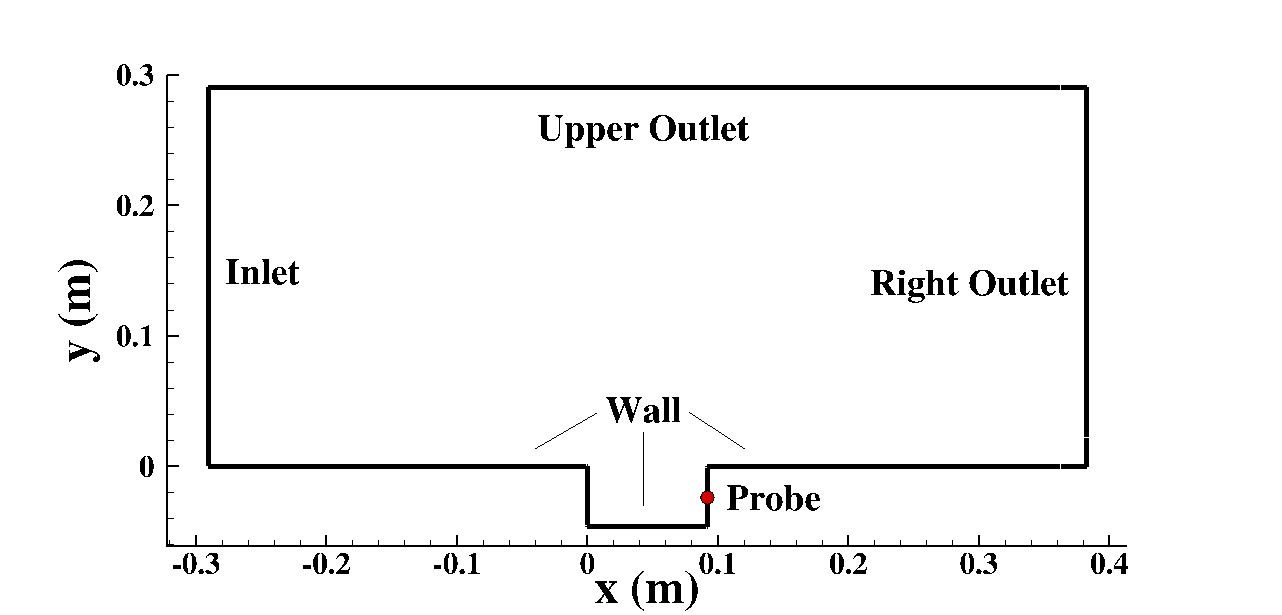
\includegraphics[width=0.9\linewidth]{Chapters/HPROMResults/Images/cavity/geom.png}
    \caption{\label{fig:cavityGeom}Cavity flow domain.}
\end{figure}

The working fluid is air, modeled as a calorically-perfect gas with the properties given in Table~\ref{tab:airProps}. Transport and thermodynamic properties are computed using the simplified analytical forms described in Section~\ref{subsec:gasModels}. The free-stream velocity is 208.7816 m/s in the +$x$-direction, the pressure is 25 Pa, and the temperature is 300 K. The resulting Mach number of this flow regime is approximately 0.6, and the Reynolds number based on the cavity length is approximately 6,500.

\begin{table}
	\centering
	\begin{tabular}{ lllll }
	\toprule
	MW (g/mol) & $c_p$ (kJ/kg-K) & $\mu$ (kg/m-s) & Pr & Sc   \\
	\midrule
	28.9604 & 1004.84 & 8.46e-7 & 0.72 & 0.62 \\
	\bottomrule
	\end{tabular}
	\caption{\label{tab:airProps}CPG properties of air for cavity flow case.}
\end{table}

The FOM is initialized with free stream conditions outside the cavity, and the inside of the cavity is initialized with free stream pressure and temperature, and zero velocity. The physical time step for the FOM simulation is $\dtFOM = 1 \;\mu$s. Initial transients are allowed to dissipate and statistically-steady flow is established over 100 ms. After this point, the simulation is continued for 10 ms, during which the state is saved to disk at every physical time step, resulting in 10,001 snapshots (including $\stateVec\left(\timeVar = 100 \; \text{ms}\right)$). All PROM simulations are restarted from $\timeVar = 100 \; \text{ms}$. Several instantaneous flow field examples are shown in Figs.~\ref{fig:cavityPressExample}--\ref{fig:cavityVExampleZoom}. Particular attention is drawn to the oscillatory pressure field displayed in Fig.~\ref{fig:cavityPressExample}: this emission of pressure waves from the trailing edge of the cavity is the result of the shear layer (originating from leading edge) impinging on the trailing edge. The shear layer rollup (implied by the $y$-velocity field in Fig.~\ref{fig:cavityVExampleZoom}) due to the Helmholtz instability and the pressure perturbation that travels upstream results in several resonant tones. Pressure measurements at the aft wall over the 10 ms data collection period is shown in Fig.~\ref{fig:cavityFOMProbe}.

\begin{figure}
	\centering
	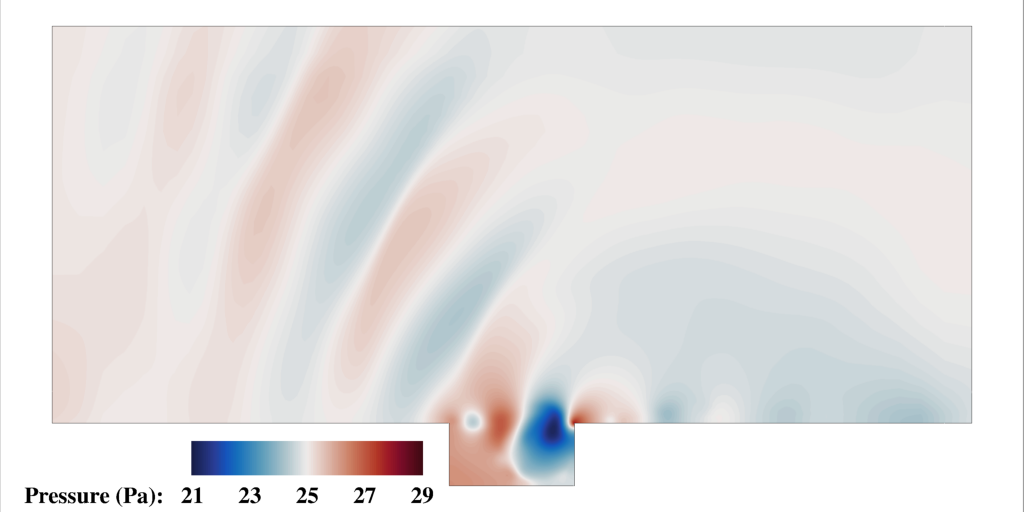
\includegraphics[width=0.9\linewidth,trim={0.5em 0.5em 0.5em 0.5em},clip]{Chapters/HPROMResults/Images/cavity/pressure_example_full.png}
	\caption{\label{fig:cavityPressExample}Cavity pressure field at $\timeVar =$ 104 ms.}
\end{figure}

\begin{figure}
	\begin{minipage}{0.48\linewidth}
		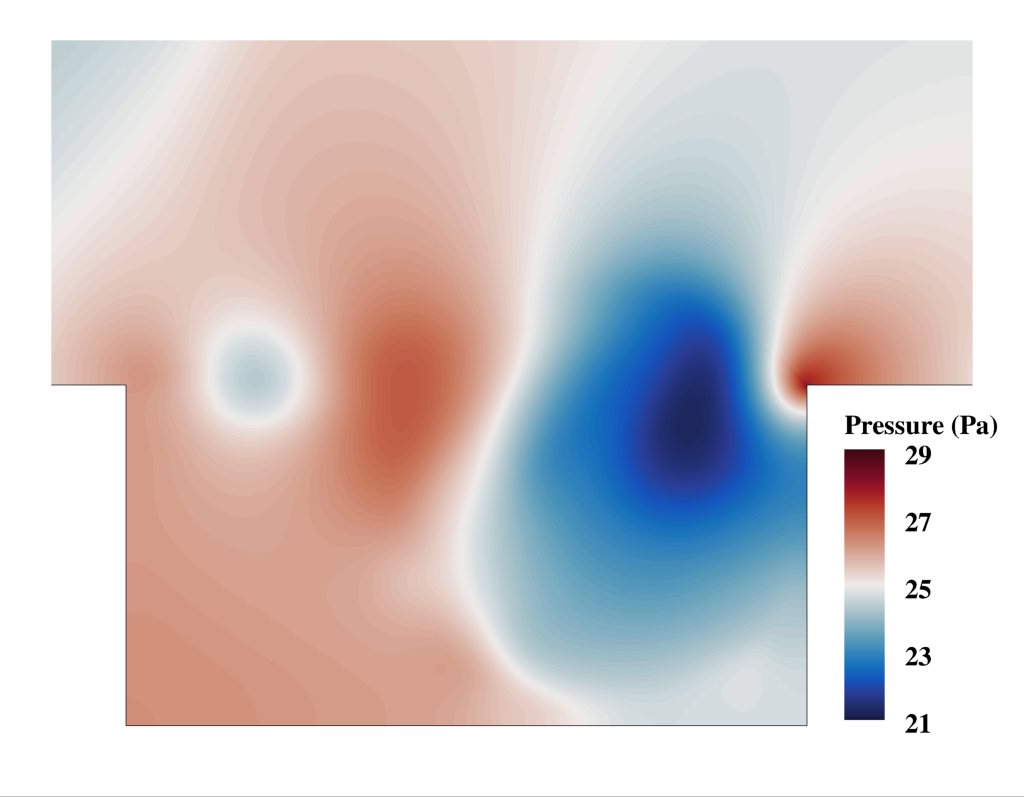
\includegraphics[width=0.99\linewidth,trim={0.5em 0.5em 0.5em 0.5em},clip]{Chapters/HPROMResults/Images/cavity/pressure_example_zoom.png}
		\caption{\label{fig:cavityPressExampleZoom}Cavity pressure field at $\timeVar =$ 104 ms, zoomed view.}
	\end{minipage} \hspace{0.5em}
	\begin{minipage}{0.48\linewidth}
		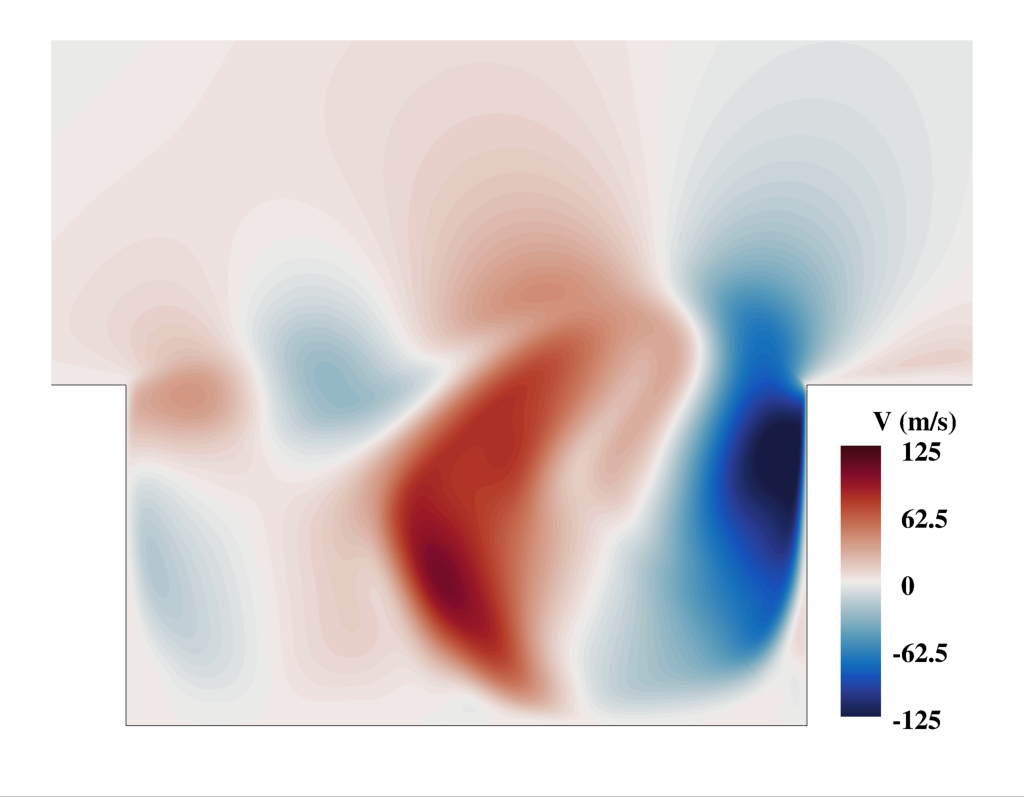
\includegraphics[width=0.99\linewidth,trim={0.5em 0.5em 0.5em 0.5em},clip]{Chapters/HPROMResults/Images/cavity/y_vel_example_zoom.png}
		\caption{\label{fig:cavityVExampleZoom}Cavity $y$-velocity field at $\timeVar =$ 104 ms, zoomed view.}
	\end{minipage}
\end{figure}

For this flow regime and cavity geometry, the formula of Rossiter~\cite{Rossiter1964} (with $\alpha = 0.25$, $\kappa = 0.57$) predicts the first three acoustic modes to be $f = \{725.2, \; 1,692.1, \; 2,659.1\}$ Hz. As a rough confirmation of model suitability, 100 ms ($\timeVar \in [100, \; 200]$ ms) of pressure data are collected from the aft wall point monitor. The signal is filtered using a low-pass fifth-order Butterworth filter with a critical frequency of 20 kHz, and the power spectral density is computed by Welch's method with a window of 25 ms and 75\% window overlap. The resulting sound pressure level is plotted in Fig.~\ref{fig:rossiterModeProof}, where the first three predicted Rossiter frequencies are marked in red. Although slightly overpredicting the first mode and underpredicting the third mode, this is a reasonable match in comparing an empirical fit model and a two-dimensional numerical simulation.

\begin{figure}
	\begin{minipage}{0.48\linewidth}
		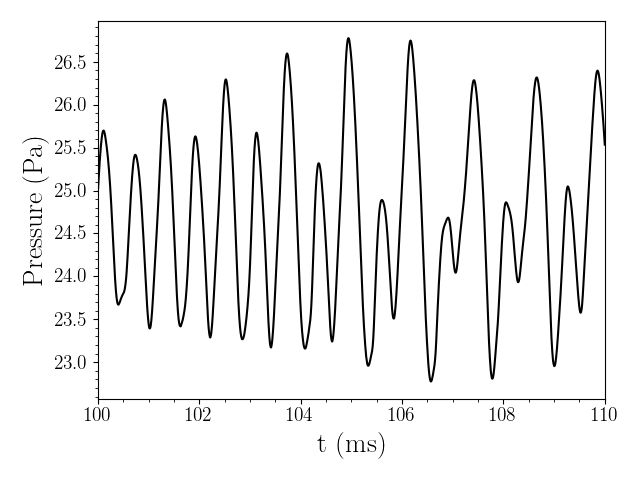
\includegraphics[width=0.99\linewidth,trim={0.5em 0.5em 0.5em 0.5em},clip]{Chapters/HPROMResults/Images/cavity/pressure_probe_fom_10ms.png}
		\caption{\label{fig:cavityFOMProbe}Pressure probe measurements from aft wall ($\timeVar \in [100, \; 110]$ ms).}
	\end{minipage} \hspace{0.5em}
	\begin{minipage}{0.48\linewidth}
		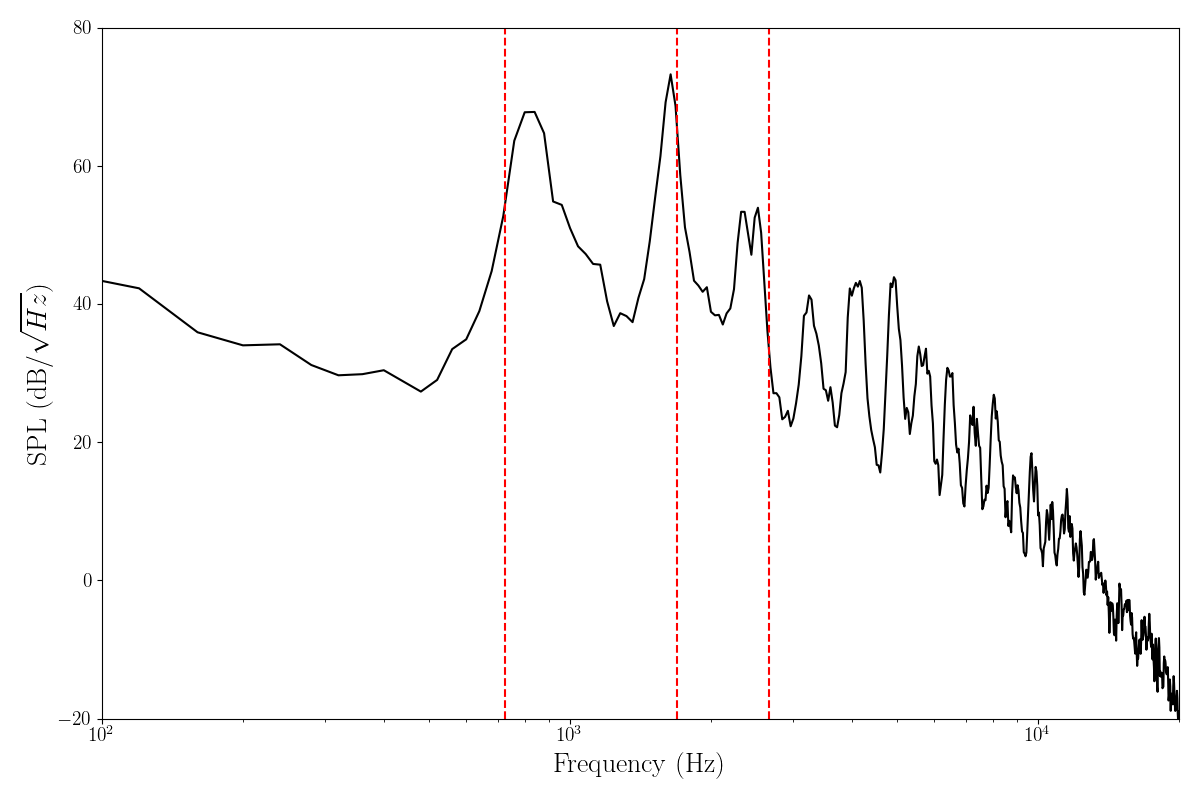
\includegraphics[width=0.99\linewidth,trim={0.5em 0.5em 0.5em 0.5em},clip]{Chapters/HPROMResults/Images/cavity/psd_fom_100ms.png}
		\caption{\label{fig:rossiterModeProof}Sound pressure level of aft wall pressure signal ($\timeVar \in [100, \; 200]$ ms). The first three Rossiter frequencies are marked in red.}
	\end{minipage}
\end{figure}

The POD trial bases are computed from the 10,001 snapshots of the conservative and primitive variables. The POD residual energy decay is displayed in Fig.~\ref{fig:cavityPODEnergy}. Achieving 1\%, 0.1\%, and 0.01\% of the conservative state POD residual energy requires 20, 73, and 155 modes respectively. For the primitive state, this increases to 26, 92, and 180 modes respectively. Although this is a fairly simple problem without any reaction phenomena, this slow POD residual energy decay exhibits how traveling waves and large fluctuations in the unsteady flow field can require a large number of trial bases to approximate accurately. Indeed, the primitive and conservative variable projection error plots in Fig.~\ref{fig:cavityProjErr} indicate that over 125 modes are required to decrease the projection error of velocity and momentum magnitudes below 0.1\% relative error.

\begin{figure}
	\centering
	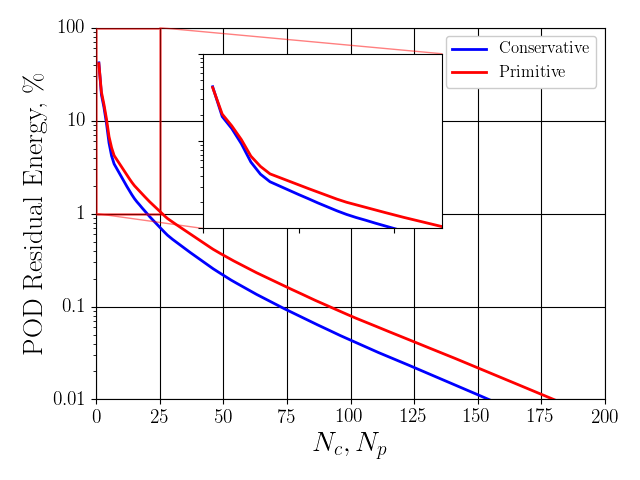
\includegraphics[width=0.75\linewidth]{Chapters/HPROMResults/Images/cavity/cavity_pod_energy_10ms.png}
	\caption{\label{fig:cavityPODEnergy}Cavity POD residual energy for conservative and primitive state datasets.}
\end{figure}

\begin{figure}
	\begin{minipage}{0.49\linewidth}
		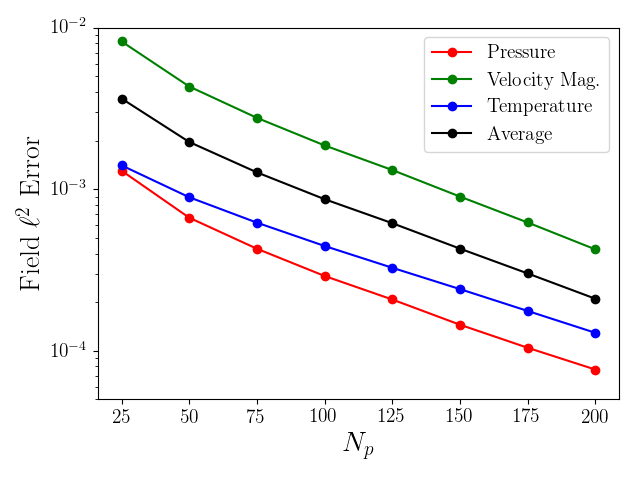
\includegraphics[width=0.99\linewidth,trim={0.5em 0.5em 0.5em 0.5em},clip]{Chapters/HPROMResults/Images/cavity/projection_error_primitive.png}
		\subcaption{Primitive variables}
	\end{minipage}
	\begin{minipage}{0.49\linewidth}
		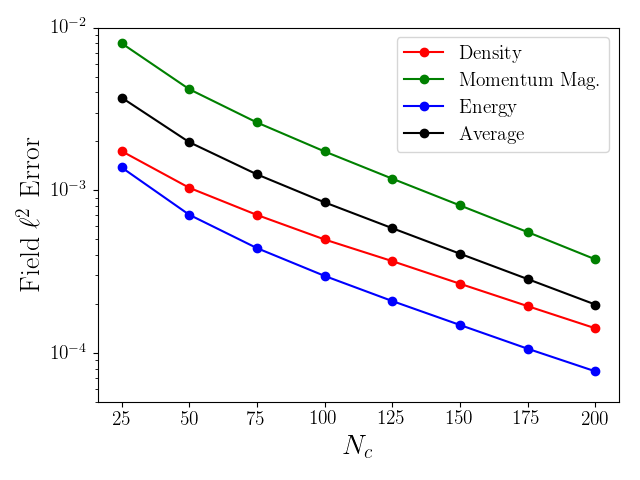
\includegraphics[width=0.99\linewidth,trim={0.5em 0.5em 0.5em 0.5em},clip]{Chapters/HPROMResults/Images/cavity/projection_error_conservative.png}
		\subcaption{Conservative variables}
	\end{minipage}
	\caption{\label{fig:cavityProjErr}Cavity time-average POD projection error.}
\end{figure}

\subsection{Unsampled PROMs}

The performance of unsampled Galerkin, LSPG, and MP-LSVT PROMs is examined first. As mentioned previously, the application of projection-based ROMs alone does not result in computational cost reduction, but still serves as a good performance baseline. If the unsampled PROM performs poorly, the hyper-reduced PROM can hardly be expected to perform well.

A trial basis dimension study and time step size study is conducted. The trial basis dimension $\numConsModes$/$\numPrimModes$ is swept from 25 modes to 200 modes at 25-mode intervals. Four time step sizes are examined: $\Delta \timeVar \in \{ 1, \; 2.5, \; 5, \; 10 \} \; \mu \text{s}$, or 1, 2.5, 5, and 10 times that of the FOM simulation. As has been documented by previous work~\cite{Carlberg2017,Huang2022,Wentland2021}, increasing the PROM time step often achieves computational speedup with negligible increase in error relative to PROMs for which $\dt = \dtFOM$, up to a point. Average error results for each evaluated time step are displayed in Fig.~\ref{fig:cavityUnsampledROMErrVsModes}. Several indicative pressure probe measurements are displayed in Fig.~\ref{fig:cavityUnsampledROMProbes}.

\begin{figure}
	\begin{minipage}{0.49\linewidth}
		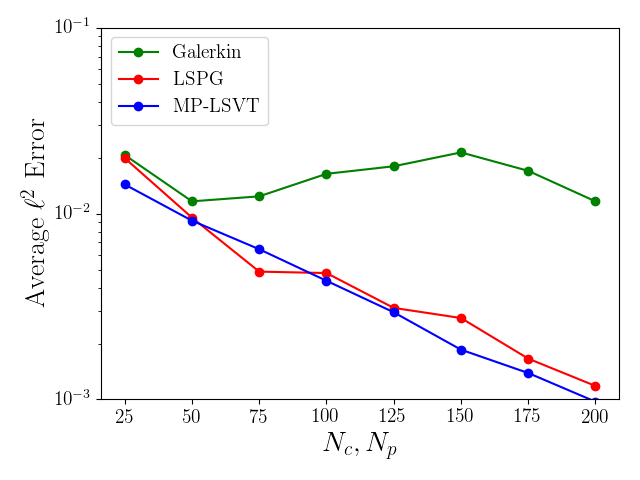
\includegraphics[width=0.99\linewidth]{Chapters/HPROMResults/Images/cavity/unsampled/unsampled_dt1e-6_Average_errorRaw.png}
		\subcaption{$\dt = \dtFOM$}
	\end{minipage}
	\begin{minipage}{0.49\linewidth}
		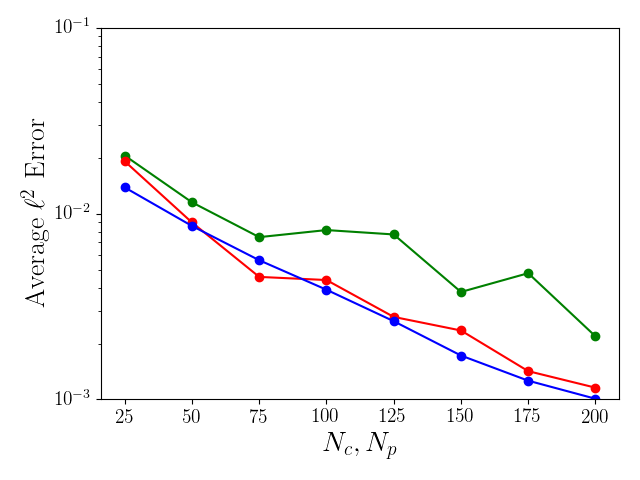
\includegraphics[width=0.99\linewidth]{Chapters/HPROMResults/Images/cavity/unsampled/unsampled_dt2p5e-6_Average_errorRaw.png}
		\subcaption{$\dt = 2.5 \times \dtFOM$}
	\end{minipage}

	\begin{minipage}{0.49\linewidth}
		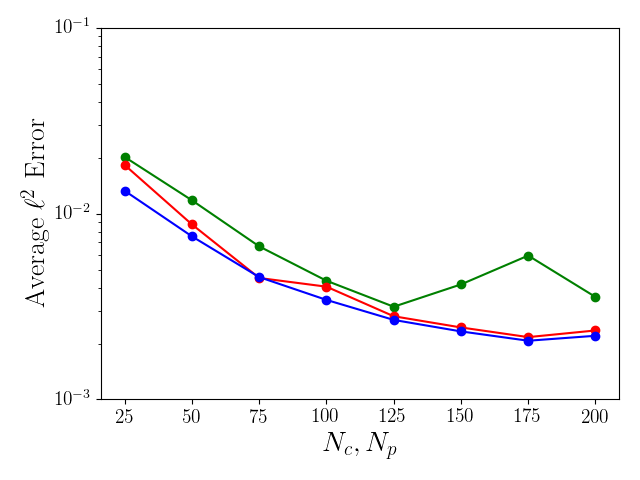
\includegraphics[width=0.99\linewidth]{Chapters/HPROMResults/Images/cavity/unsampled/unsampled_dt5e-6_Average_errorRaw.png}
		\subcaption{\label{fig:cavityUnsampledROMErrVsModesDt5en6}$\dt = 5 \times \dtFOM$}
	\end{minipage}
	\begin{minipage}{0.49\linewidth}
		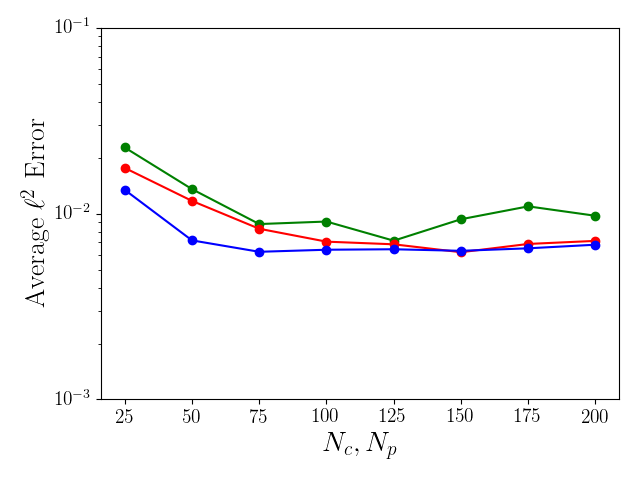
\includegraphics[width=0.99\linewidth]{Chapters/HPROMResults/Images/cavity/unsampled/unsampled_dt1e-5_Average_errorRaw.png}
		\subcaption{$\dt = 10 \times \dtFOM$}
	\end{minipage}
	\caption{\label{fig:cavityUnsampledROMErrVsModes}Cavity unsampled PROM time-average error, various $\dt$.}
\end{figure}

\begin{figure}
	\begin{minipage}{0.49\linewidth}
		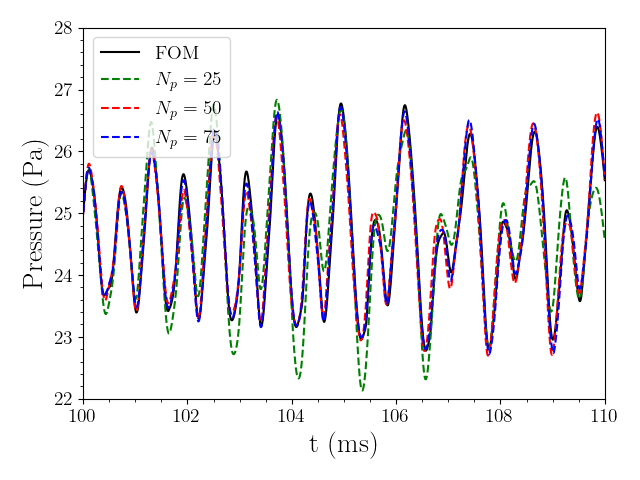
\includegraphics[width=0.99\linewidth]{Chapters/HPROMResults/Images/cavity/unsampled/pressure_probe_unsampled_modes.png}
		\subcaption{\label{fig:cavityUnsampledROMProbesModes}MP-LSVT method, various $\numPrimModes$.}
	\end{minipage}
	\begin{minipage}{0.49\linewidth}
		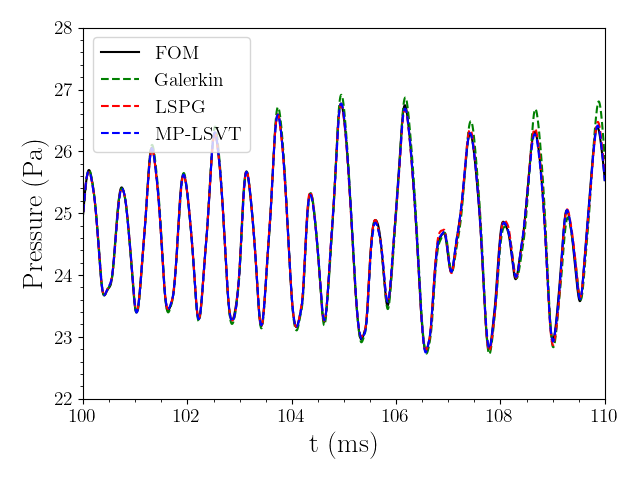
\includegraphics[width=0.99\linewidth]{Chapters/HPROMResults/Images/cavity/unsampled/pressure_probe_unsampled_methods.png}
		\subcaption{\label{fig:cavityUnsampledROMProbesMethods}$\numConsModes,\numPrimModes$ = 150, various methods.}
	\end{minipage}
	\caption{\label{fig:cavityUnsampledROMProbes}Cavity unsampled PROM probe measurements, $\dt = 5 \times \dtFOM$.}
\end{figure}

Unremarkably, the LSPG and MP-LSVT PROMs outperform the Galerkin PROMs at all mode counts and time steps. Further, the LSPG and MP-LSVT PROMs generally exhibit non-increasing accuracy with trial basis enrichment, while error often \textit{increases} with trial basis enrichment for the Galerkin PROMs. For all time steps and trial basis dimensions evaluated, the LSPG and MP-LSVT PROMs perform similarly. This is not unexpected, as this is a non-reacting simulation which does not involve stiff source terms, extremely disparate spatio-temporal scales, or poor conditioning from which traditional LSPG PROMs might suffer. As mentioned previously, increasing the PROM time step may result in ``free'' computational cost savings. Indeed, increasing the PROM time step to $\dt = 2.5 \times \dtFOM$ generates virtually no error increase for the LSPG and MP-LSVT PROMs, and even improves the performance of the Galerkin PROMs. However, at higher time step sizes, the accuracy of all PROMs for roughly $\numConsModes$, $\numPrimModes > 50$ deteriorate drastically. In fact, for $\dt = 10 \times \dtFOM$, accuracy improvement via trial basis enrichment saturates at $\numConsModes$, $\numPrimModes = 50$, never dropping below 0.5\%.

The pressure probe monitors in Fig.~\ref{fig:cavityUnsampledROMProbes} display largely unsurprising results. As seen in Fig~\ref{fig:cavityUnsampledROMProbesModes}, a very low trial basis dimension ($\numPrimModes = 25$), the solution quickly deviates and fails to reconstruct the FOM data faithfully. Large over- and under-shoot in the unsteady pressure signal are observed, and by the end of the simulation period the signal has devolved into small, unorganized fluctuations. Increasing the resolution to $\numPrimModes = 50$ improves the signal reconstruction, although small under- and over-shoot is observed by $\timeVar = 103$ ms. This small discrepancy is only marginally improved by increasing the trial basis dimension to $\numPrimModes = 75$, in agreement with the converging average error shown in Fig.~\ref{fig:cavityUnsampledROMErrVsModesDt5en6}.

\begin{figure}
    \centering
    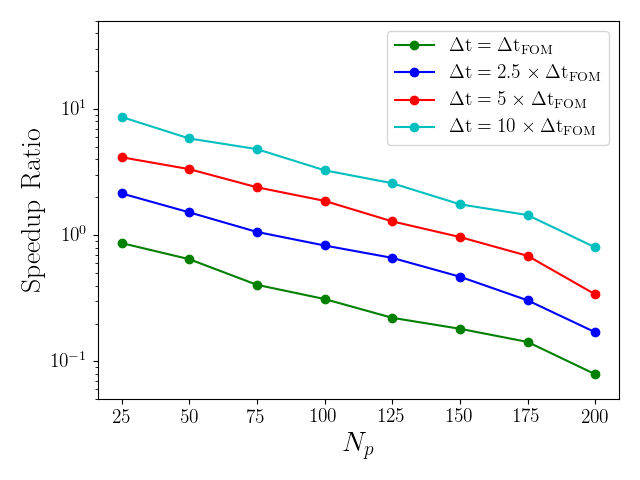
\includegraphics[width=0.7\linewidth]{Chapters/HPROMResults/Images/cavity/unsampled/unsampled_modeStudy_time_calcAndMPI.png}
    \caption{\label{fig:cavityUnsampledCost}MP-LSVT unsampled PROM computational cost, relative to FOM cost, various $\dt$.}
\end{figure}

The computational cost of the unsampled MP-LSVT PROMs is now examined. Results are nearly identical for equivalent Galerkin and LSPG PROMS. As discussed previously, projection-based ROMs \textit{alone} should not produce any significant computational cost savings, and in fact should increase cost due to lifting the state to the full-dimension and projecting the non-liner function onto the test space. Figure~\ref{fig:cavityUnsampledCost} quantifies just how much this change affects the run-time of the unsampled PROM. Note that using the same time step size as that of the FOM, the unsampled PROM is always more expensive than the FOM (below 1 on the $y$-axis) no matter the trial basis dimension. This highlights the necessity of hyper-reduction: projection-based order reduction of the governing system alone, even for extremely low trial/test basis dimensions, does not improve PROM computational cost. For $\dt = 2.5 \times \dtFOM$, the unsampled PROM only achieves speedup for $\numPrimModes < 100$. This trend continues to improve the speedup for $\dt = 5 \times \dtFOM, \; 10 \times \dtFOM$, though prior results showed that PROM accuracy quickly deteriorates at high time steps. For $\numPrimModes = 100$ and $\dt = 10 \times \dtFOM$, the unsampled PROM is only capable of achieving three times speedup, which is hardly impressive given that these results only reconstruct the training period. To realize significant cost savings, hyper-reduction must be applied.

\subsection{Hyper-reduced PROMs}
%
For the sake of brevity, only MP-LSVT HPROMs are examined. As will be seen in Section~\ref{sec:cvrc}, Galerkin and LSPG PROMs appear unsuitable for practical reacting flows, and will not be discussed thereafter. All results presented in this section utilize a trial basis dimension of $\numPrimModes = 150$. All gappy POD regressor bases are constructed from POD modes of the conservative field dataset, i.e., $\deimBasis = \consTrial \inRTwo{\numDOF}{\numResModes}$, as detailed in Section~\ref{subsec:stateApproxDEIM}

\begin{figure}
	\begin{minipage}{0.49\linewidth}
		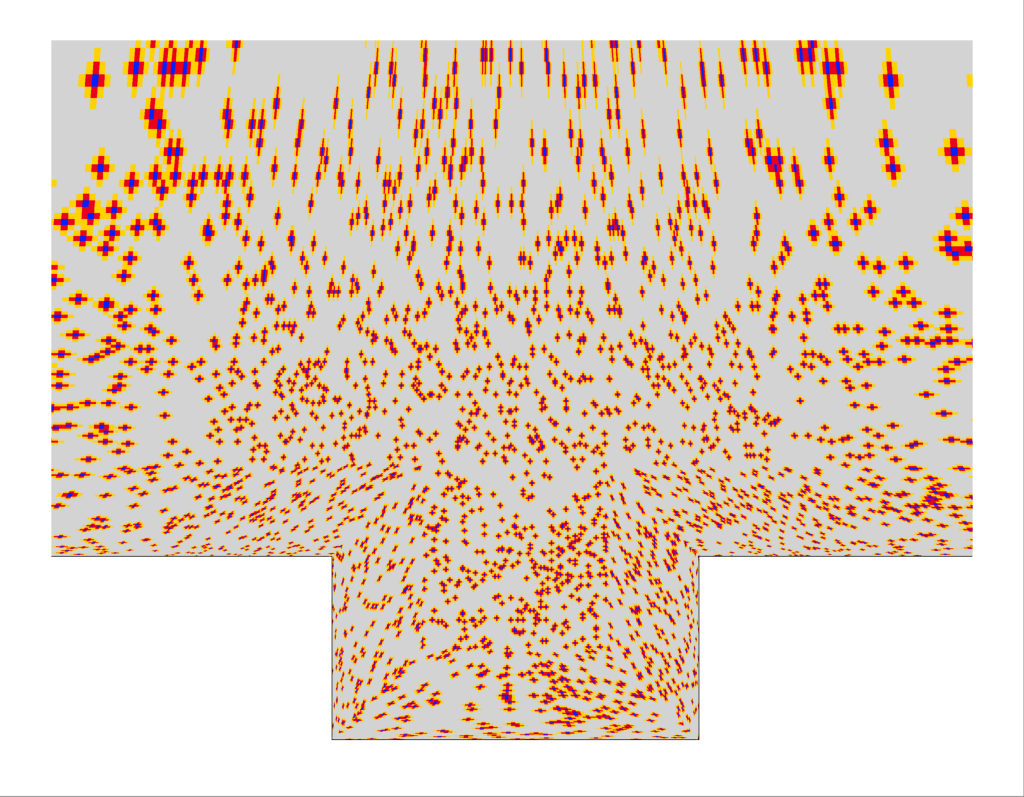
\includegraphics[width=0.99\linewidth,trim={0.5em 0.5em 0.5em 0.5em},clip]{Chapters/HPROMResults/Images/cavity/deim/iBlank_random_zoom.png}
		\subcaption{Random}
	\end{minipage}
	\begin{minipage}{0.49\linewidth}
		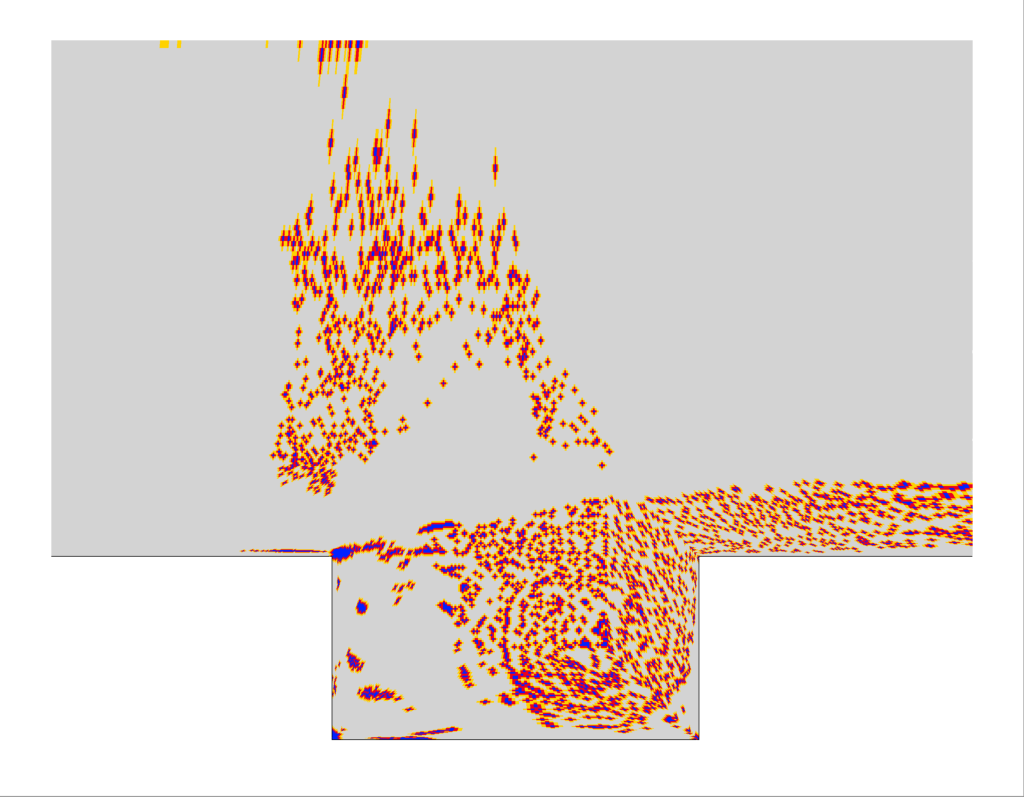
\includegraphics[width=0.99\linewidth,trim={0.5em 0.5em 0.5em 0.5em},clip]{Chapters/HPROMResults/Images/cavity/deim/iBlank_eigenvec_zoom.png}
		\subcaption{Eigenvector}
	\end{minipage}

	\begin{minipage}{0.49\linewidth}
		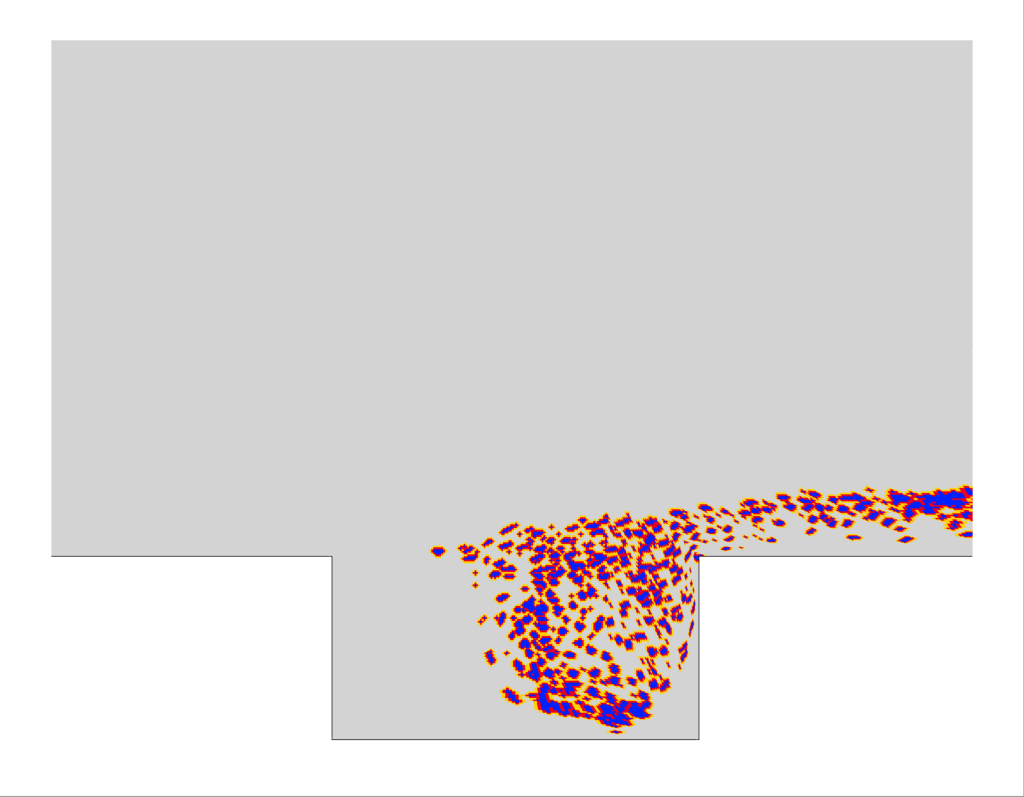
\includegraphics[width=0.99\linewidth,trim={0.5em 0.5em 0.5em 0.5em},clip]{Chapters/HPROMResults/Images/cavity/deim/iBlank_greedy_carlberg_zoom.png}
		\subcaption{GNAT V1}
	\end{minipage}
	\begin{minipage}{0.49\linewidth}
		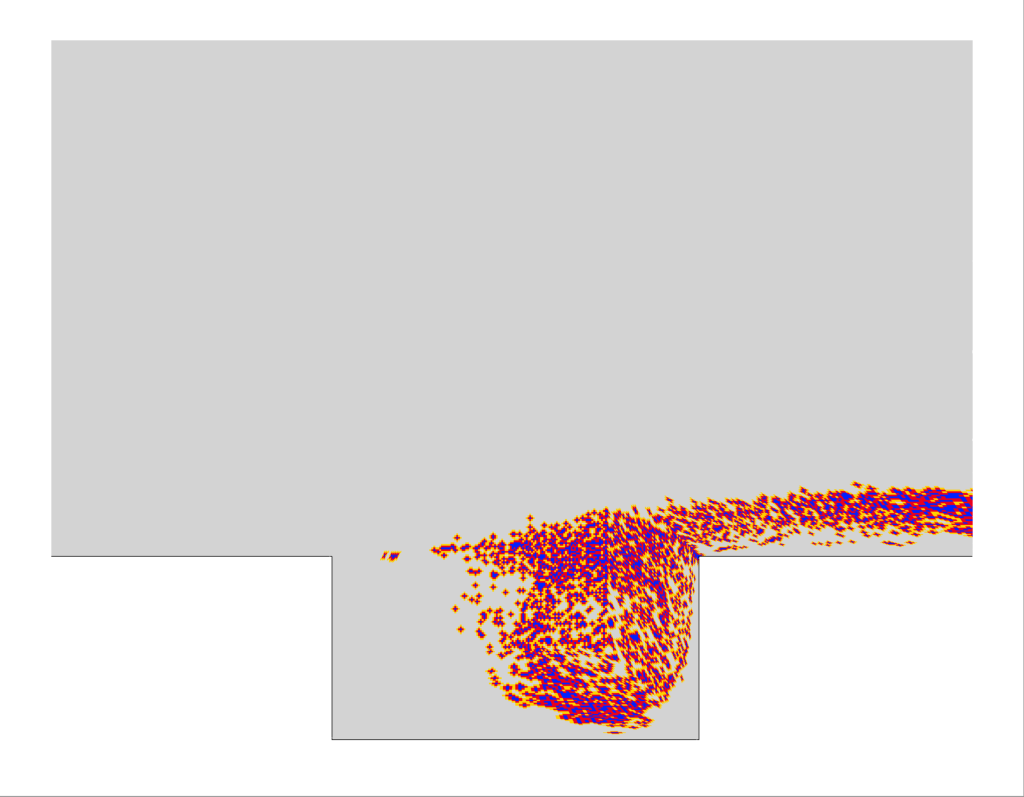
\includegraphics[width=0.99\linewidth,trim={0.5em 0.5em 0.5em 0.5em},clip]{Chapters/HPROMResults/Images/cavity/deim/iBlank_greedy_ben_zoom.png}
		\subcaption{GNAT V2}
	\end{minipage}
	\caption{\label{fig:cavityiBlank}Cavity sample mesh examples, $\numResModes= 250$, $\numSamps = 2.5\% \times \numDOF$.}
\end{figure}

\begin{table}
	\centering
	\begin{tabular}{ llllllllll }
	\toprule
	Sampling Rate (\%) & 0.5 & 0.75 & 1 & 1.75 & 2.5 & 3.75 & 5.0 & 7.5 & 10 \\
	\midrule
	Cores & 2 & 2 & 2 & 2 & 3 & 5 & 6 & 9 & 13 \\
	Cells/core (approx.) & 312 & 469 & 625 & 1,093 & 1,042 & 938 & 1,042 & 1,042 & 962 \\
	\bottomrule
	\end{tabular}
	\caption{\label{tab:cavitySampProcs}Partitioning for cavity HPROM sample meshes.}
\end{table}

The accuracy and computational performance of the HPROMs is examined for sampling rates of $\numSamps \in \{0.5, \; 0.75, \; 1.0, \; 1.75, \; 2.5, \; 3.75, \; 5.0, \; 7.5, \; 10\}\% \times \numDOF$, and gappy POD regressor dimensions of $\numResModes \in \{150, \; 200, \; 250, \; 300\}$. Views of indicative sample meshes constructed using the four sampling algorithms detailed in Section~\ref{subsec:sampAlgos} are shown in Fig.~\ref{fig:cavityiBlank}. As in Section~\ref{sec:sampleMesh}, blue cells indicate directly-sampled cells, red cells indicate flux cells, and yellow cells indicate gradient/vertex cells. The three greedy sampling algorithms generate sample meshes which are quite similar in some ways: the vast majority of sampled cells are located in the shear layer originating from the cavity leading edge and meandering downstream, as well as in the strong recirculation region in the downstream half of the cavity. The most glaring difference appears to be that the eigenvector-based algorithm also selects a number of points in the free-stream flow. Note that this region, although dominated by the free-stream conditions, experiences strong pressure oscillations emitted from the cavity trailing edge. Interestingly, the GNAT V1 algorithm selects sample cells in extremely tight clusters, while GNAT V2 generates a relatively more diffuse sample mesh, and the eigenvector-based algorithm's sample mesh is even more diffuse. Further, the eigenvector-based sampling selects a significant number of points on the leading edge of the cavity and in the upstream half of the cavity. It will be shown shortly how apparently minor discrepancies can have a drastic effect on HPROM performance. For all online HPROM results, each sample mesh is partitioned for parallel computations according to the sampling rate, as given in Table~\ref{tab:cavitySampProcs}, regardless of the sampling algorithm utilized. The number of cores is altered for each sampling rate to ensure approximately equal load balancing, amounting to roughly 1,000 cells per core. Note that this is impossible for $\numSamps \le 1\% \times \numDOF$, and two cores are used for such cases.

\begin{figure}
	\begin{minipage}{0.46\linewidth}
		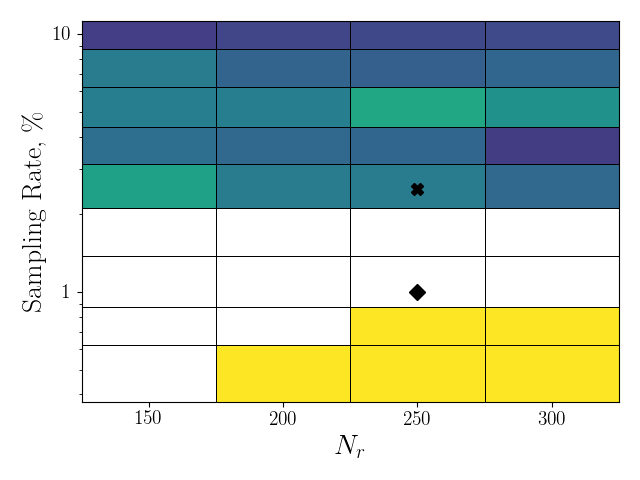
\includegraphics[width=0.99\linewidth]{Chapters/HPROMResults/Images/cavity/deim/err_contour_random_dt5e-6.png}
		\subcaption{Random}
	\end{minipage}
	\begin{minipage}{0.53\linewidth}
		\includegraphics[width=0.99\linewidth]{Chapters/HPROMResults/Images/cavity/deim/err_contour_eigenvec_dt5e-6.png}
		\subcaption{Eigenvector}
	\end{minipage}

	\begin{minipage}{0.46\linewidth}
		\includegraphics[width=0.99\linewidth]{Chapters/HPROMResults/Images/cavity/deim/err_contour_gnat1_dt5e-6.png}
		\subcaption{GNAT, V1}
	\end{minipage}
	\begin{minipage}{0.53\linewidth}
		\includegraphics[width=0.99\linewidth]{Chapters/HPROMResults/Images/cavity/deim/err_contour_gnat2_dt5e-6.png}
		\subcaption{GNAT, V2}
	\end{minipage}
	\caption{\label{fig:cavitySampledROMErrContour}Cavity HPROM time-average error contours with respect to gappy POD regressor dimension and sampling rate, $\dt = 5 \times \dtFOM$, various sampling algorithms.}
\end{figure}

The accuracy of the online HPROMs on sample meshes generated by each sampling algorithm stand in stark contrast. Time-average $\ell^2$ error contour plots for $\dt = 5 \times \dtFOM$ are given in Fig.~\ref{fig:cavitySampledROMErrContour},comparing accuracy at each combination of sampling rate $\numSamps$ and gappy POD regressor basis dimension $\numResModes$. White squares indicate simulations which exploded. Across all sampling algorithms, note the unsurprising result that increasing $\numSamps$ and $\numResModes$ tends to improve HPROM performance. However, it is quite plain that eigenvector-based sampling consistently generates more stable and accurate HPROMs than any other sampling algorithm, only failing at extremely low sampling rates. Interestingly, random sampling tends to outperform both GNAT sampling algorithms, though it only produces stable simulations for $\numSamps > 2.5\% \times \numDOF$. In fact, GNAT V1 produces consistently stable simulations only for $\numSamps = 10\% \times \numDOF$, and even those are highly inaccurate. The GNAT V2 algorithm is capable of producing stable simulations at lower sampling rates, but also incurs relatively high error in the solution.

\begin{figure}
	\begin{minipage}{0.49\linewidth}
		\includegraphics[width=0.99\linewidth]{Chapters/HPROMResults/Images/cavity/deim/sampled_dt2p5e-6_Average_errorRaw_pareto.png}
		\subcaption{$\dt = 2.5 \times \dtFOM$}
	\end{minipage}
	\begin{minipage}{0.49\linewidth}
		\includegraphics[width=0.99\linewidth]{Chapters/HPROMResults/Images/cavity/deim/sampled_dt5e-6_Average_errorRaw_pareto.png}
		\subcaption{$\dt = 5 \times \dtFOM$}
	\end{minipage}
	% \begin{minipage}{0.49\linewidth}
	% 	\includegraphics[width=0.99\linewidth]{Chapters/HPROMResults/Images/cavity/deim/sampled_dt1e-5_Average_errorRaw_pareto.png}
	% 	\subcaption{$\dt = 10 \times \dtFOM$}
	% \end{minipage}
	\caption{\label{fig:cavitySampledROMErrVsTime}Cavity HPROM error vs. CPU-time speedup, $\numPrimModes = 150$, $\numResModes = 250$, various $\dt$.}
\end{figure}

Of course, computational cost savings is the prime objective of hyper-reduction, and an accurate HPROM does not guarantee a fast HPROM. As one might expect, increasing $\numSamps$ and $\numResModes$ increases HPROM computational cost, as will be explored more thoroughly in Section~\ref{sec:cvrc}. Figure~\ref{fig:cavitySampledROMErrVsTime} displays the time-average error with respect to the speedup ratio at each sampling rates for all sampling algorithms. The eigenvector-based sampling enables stable, accurate HPROMs which are able to achieve over 200 times computational cost savings, while the equivalent unsampled PROMs are either equally or more expensive than the FOM. Similarly, random sampling is capable of producing accurate ($<1\%$ error), though only at higher sampling rates and achieving relatively lower speedup ratios. The GNAT sampling algorithms generally fail to produce meaningful cost savings without incurring instability or high error.

\begin{figure}
	\begin{minipage}{0.49\linewidth}
		\includegraphics[width=0.99\linewidth]{Chapters/HPROMResults/Images/cavity/deim/pressure_probe_deim_2p5.png}
		\subcaption{\label{fig:cavitySampledROMProbe2p5}$\numSamps = 2.5\% \times \numDOF$}
	\end{minipage}
	\begin{minipage}{0.49\linewidth}
		\includegraphics[width=0.99\linewidth]{Chapters/HPROMResults/Images/cavity/deim/pressure_probe_deim_1.png}
		\subcaption{\label{fig:cavitySampledROMProbe1p}$\numSamps = 1\% \times \numDOF$}
	\end{minipage}
	\caption{\label{fig:cavitySampledROMProbes}Cavity MP-LSVT HPROM probe measurements, $\numPrimModes = 150$, $\numResModes = 250$, $\dt = 5 \times \dtFOM$.}
\end{figure}

To better visualize these accuracy discrepancies, Fig.~\ref{fig:cavitySampledROMProbes} displays pressure probe monitors for each sampling algorithm for two different sampling rates. The corresponding average error for Fig.~\ref{fig:cavitySampledROMProbe2p5} are marked with an ``X'' in Figs.~\ref{fig:cavitySampledROMErrContour} and~\ref{fig:cavitySampledROMErrVsTime}, and those for Fig.~\ref{fig:cavitySampledROMProbe1p} are similarly marked by a diamond. In general, all sampling algorithms are able to produce stable and accurate PROMs for the simulation period $\timeVar \in [100, \; 102]$ ms. However, those HPROMs generated by the GNAT sampling algorithms quickly deviate from the FOM, exhibiting wild swings in the unsteady pressure signal. Although random sampling generates an unstable HPROM for $\numSamps = 1\% \times \numDOF$, it produces a fairly accurate simulation for $\numSamps = 2.5\% \times \numDOF$, only exhibiting minor under- and over-shoot towards the end of the simulation period. Eigenvector-based sampling produces accurate reconstruction of the unsteady pressure signal, particularly for $\numSamps = 2.5\% \times \numDOF$, though it does exhibit some discrepancies at later times for $\numSamps = 1\% \times \numDOF$.

Although the above results indicate that it is possible to achieve excellent computational cost savings with HPROMs, they also hint at the challenge of guaranteeing that they are accurate and robust. The drastic effects that the sample mesh and gappy POD regression have on HPROM performance invites more thorough exploration for larger, more challenging systems.
\section{Continuously-variable Resonance Chamber}\label{sec:cvrc}


% \subsection{High-amplitude Pressure Wave Reconstruction}
\section{Nine-element Combustor}\label{app:nineElemSupp}
\chapter{Supplementary Results}
\label{app:suppResults}

In the author's personal experience, there is often a certain opacity in the projection-based ROM literature on the subject of data preparation and robustness controls. In many cases this is simply due to the fact that many PROM studies deal with systems which are governed by a single state variable (Burgers' equation, Kuramoto--Sivashinsky equation), are governed by state variables that are naturally of similar magnitudes (shallow water equations, Euler equations for Sod shock tube), or are commonly non-dimensionalized in open-source or commercial solvers (incompressible Navier--Stokes). In such situations, the dimensionality of the state variables is either irrelevant or has little effect on the accuracy of state representations and the solution of the PROM equations. Sometimes, however, small but crucial details of data preparation or the PROM solution are left out as they are considered self-evident to the authors (as has been discovered anecdotally by this author and colleagues). To date, the work by Parish and Rizzi~\cite{Parish2022} provides the most explicit description and comprehensive study of ensuring a dimensionally-consistent POD formulation and PROM solution by careful choice of inner products. Although the focus of their work is the compressible Euler equations, they provides broadly-meaningful insights for dimensional dynamical systems.

All but one numerical experiment in this thesis deals with high-pressure, compressible reacting flows, which are characterized by both vastly disparate magnitudes in the system state and an inability to readily non-dimensionalize the governing equations. As such, careful data preparation and unsteady solution robustness controls are extremely important in enabling the stable and accurate solution of projection-based reduced-order models. Further, this thesis aims to be as transparent about every element of the PROM construction process to help enable successful PROMs for future researchers working with similarly-complex systems. Some of the key elements in this process are detailed the numerical experiments which follow.

All results shown in this chapter are unsampled MP-LSVT PROMs of the truncated CVRC case investigated in Section~\ref{sec:cvrc}. A time step of $\dt = 5 \times \dtFOM$ is used in all cases.
\section{Transient Flame}\label{app:transientFlameSupp}


To begin this section, two-dimensional transonic flow over an open cavity is examined. Flow over open cavities has been studied extensively due to its practical applications in aviation (e.g., bomb or landing gear bays) and the interesting acoustic phenomena it exhibits, particularly the resonant coupling of the cavity leading edge shear layer and acoustic feedback from the cavity trailing edge. Pioneering experimental work in the mid-1900's such as that by Roshko~\cite{Roshko1952}, Krishnamurty~\cite{Krishnamurty1955}, and Rossiter~\cite{Rossiter1964}, numerical modeling work such as that by Colonius \textit{et al.}~\cite{Colonius1999}, Rowley \textit{et al.}~\cite{Rowley2002}, and Larchev\^{e}que \textit{et al.}~\cite{Larcheveque2007}, and more recent experimental efforts such as those by Wagner\textit{et al.}~\cite{Wagner2015} and Casper \textit{et al.}~\cite{Casper2018} have investigated the effects of cavity dimensions, freestream flow regime, and turbulence on the behavior of this aeroacoustic coupling. This work follows the research conducted by Tezaur \textit{et al.}~\cite{Tezaur2016,Tezaur2017} in investigating PROM performance in modeling two-dimensional flow over a rectangular cavity at a Mach number of 0.6.

\subsection{Full-order Model}

The computational domain is modeled as a rectangular cavity set in a flat wall, with the leftmost, rightmost, and topmost boundaries of the domain open to the atmosphere. The geometry is shown in Fig.~\ref{fig:cavityGeom}. The cavity is $L =$ 91.71 mm long, and $D =$ 45.855 mm deep ($L/D = 2.0$). The wall extends 290.8 mm (a little over three cavity lengths) both upstream and downstream of the leading and trailing edges of the cavity, respectively, for a total domain length of 673.31 mm. The upper boundary (open to air) is set 290.8 mm from the main wall. No-slip wall boundary conditions are enforced at all walls. A characteristic inlet boundary condition is enforced at the left-most domain boundary, and characteristic outlet boundary conditions are enforced at the topmost and rightmost domain boundaries. These characteristic boundaries allow acoustic waves to exit the domain with minimal reflection. The mesh is composed of 125,000 quadrilateral cells, resulting in a total number of degrees of freedom of $\numDOF =$ 500,000. A red dot in Fig.~\ref{fig:cavityGeom} marks the location of a point monitor which will be measured throughout this section. It is placed halfway up the aft wall of the cavity, at $(x, \; y) = (91.71, \; -22.93)$ mm. Note that this full-order model should not be considered a truly accurate representation of flow over an open cavity, and this thesis makes no such claims. Beyond the measurement of the acoustic content and comparison against an empirical model in Fig.~\ref{fig:rossiterModeProof}, results presented in this chapter simply aim to model the dynamics present in this approximate simulation.

\begin{figure}
    \centering
	\includegraphics[width=0.9\linewidth]{Chapters/HPROMResults/Images/cavity/geom.png}
    \caption{\label{fig:cavityGeom}Cavity flow domain.}
\end{figure}

The working fluid is air, modeled as a calorically-perfect gas with the properties given in Table~\ref{tab:airProps}. Transport and thermodynamic properties are computed using the simplified analytical forms described in Section~\ref{subsec:gasModels}. The free-stream velocity is 208.7816 m/s in the +$x$-direction, the pressure is 25 Pa, and the temperature is 300 K. The resulting Mach number of this flow regime is approximately 0.6, and the Reynolds number based on the cavity length is approximately 6,500.

\begin{table}
	\centering
	\begin{tabular}{ lllll }
	\toprule
	MW (g/mol) & $c_p$ (kJ/kg-K) & $\mu$ (kg/m-s) & Pr & Sc   \\
	\midrule
	28.9604 & 1004.84 & 8.46e-7 & 0.72 & 0.62 \\
	\bottomrule
	\end{tabular}
	\caption{\label{tab:airProps}CPG properties of air for cavity flow case.}
\end{table}

The FOM is initialized with free stream conditions outside the cavity, and the inside of the cavity is initialized with free stream pressure and temperature, and zero velocity. The physical time step for the FOM simulation is $\dtFOM = 1 \;\mu$s. Initial transients are allowed to dissipate and statistically-steady flow is established over 100 ms. After this point, the simulation is continued for 10 ms, during which the state is saved to disk at every physical time step, resulting in 10,001 snapshots (including $\stateVec\left(\timeVar = 100 \; \text{ms}\right)$). All PROM simulations are restarted from $\timeVar = 100 \; \text{ms}$. Several instantaneous flow field examples are shown in Figs.~\ref{fig:cavityPressExample}--\ref{fig:cavityVExampleZoom}. Particular attention is drawn to the oscillatory pressure field displayed in Fig.~\ref{fig:cavityPressExample}: this emission of pressure waves from the trailing edge of the cavity is the result of the shear layer (originating from leading edge) impinging on the trailing edge. The shear layer rollup (implied by the $y$-velocity field in Fig.~\ref{fig:cavityVExampleZoom}) due to the Helmholtz instability and the pressure perturbation that travels upstream results in several resonant tones. Pressure measurements at the aft wall over the 10 ms data collection period is shown in Fig.~\ref{fig:cavityFOMProbe}.

\begin{figure}
	\centering
	\includegraphics[width=0.9\linewidth,trim={0.5em 0.5em 0.5em 0.5em},clip]{Chapters/HPROMResults/Images/cavity/pressure_example_full.png}
	\caption{\label{fig:cavityPressExample}Cavity pressure field at $\timeVar =$ 104 ms.}
\end{figure}

\begin{figure}
	\begin{minipage}{0.48\linewidth}
		\includegraphics[width=0.99\linewidth,trim={0.5em 0.5em 0.5em 0.5em},clip]{Chapters/HPROMResults/Images/cavity/pressure_example_zoom.png}
		\caption{\label{fig:cavityPressExampleZoom}Cavity pressure field at $\timeVar =$ 104 ms, zoomed view.}
	\end{minipage} \hspace{0.5em}
	\begin{minipage}{0.48\linewidth}
		\includegraphics[width=0.99\linewidth,trim={0.5em 0.5em 0.5em 0.5em},clip]{Chapters/HPROMResults/Images/cavity/y_vel_example_zoom.png}
		\caption{\label{fig:cavityVExampleZoom}Cavity $y$-velocity field at $\timeVar =$ 104 ms, zoomed view.}
	\end{minipage}
\end{figure}

For this flow regime and cavity geometry, the formula of Rossiter~\cite{Rossiter1964} (with $\alpha = 0.25$, $\kappa = 0.57$) predicts the first three acoustic modes to be $f = \{725.2, \; 1,692.1, \; 2,659.1\}$ Hz. As a rough confirmation of model suitability, 100 ms ($\timeVar \in [100, \; 200]$ ms) of pressure data are collected from the aft wall point monitor. The signal is filtered using a low-pass fifth-order Butterworth filter with a critical frequency of 20 kHz, and the power spectral density is computed by Welch's method with a window of 25 ms and 75\% window overlap. The resulting sound pressure level is plotted in Fig.~\ref{fig:rossiterModeProof}, where the first three predicted Rossiter frequencies are marked in red. Although slightly overpredicting the first mode and underpredicting the third mode, this is a reasonable match in comparing an empirical fit model and a two-dimensional numerical simulation.

\begin{figure}
	\begin{minipage}{0.48\linewidth}
		\includegraphics[width=0.99\linewidth,trim={0.5em 0.5em 0.5em 0.5em},clip]{Chapters/HPROMResults/Images/cavity/pressure_probe_fom_10ms.png}
		\caption{\label{fig:cavityFOMProbe}Pressure probe measurements from aft wall ($\timeVar \in [100, \; 110]$ ms).}
	\end{minipage} \hspace{0.5em}
	\begin{minipage}{0.48\linewidth}
		\includegraphics[width=0.99\linewidth,trim={0.5em 0.5em 0.5em 0.5em},clip]{Chapters/HPROMResults/Images/cavity/psd_fom_100ms.png}
		\caption{\label{fig:rossiterModeProof}Sound pressure level of aft wall pressure signal ($\timeVar \in [100, \; 200]$ ms). The first three Rossiter frequencies are marked in red.}
	\end{minipage}
\end{figure}

The POD trial bases are computed from the 10,001 snapshots of the conservative and primitive variables. The POD residual energy decay is displayed in Fig.~\ref{fig:cavityPODEnergy}. Achieving 1\%, 0.1\%, and 0.01\% of the conservative state POD residual energy requires 20, 73, and 155 modes respectively. For the primitive state, this increases to 26, 92, and 180 modes respectively. Although this is a fairly simple problem without any reaction phenomena, this slow POD residual energy decay exhibits how traveling waves and large fluctuations in the unsteady flow field can require a large number of trial bases to approximate accurately. Indeed, the primitive and conservative variable projection error plots in Fig.~\ref{fig:cavityProjErr} indicate that over 125 modes are required to decrease the projection error of velocity and momentum magnitudes below 0.1\% relative error.

\begin{figure}
	\centering
	\includegraphics[width=0.75\linewidth]{Chapters/HPROMResults/Images/cavity/cavity_pod_energy_10ms.png}
	\caption{\label{fig:cavityPODEnergy}Cavity POD residual energy for conservative and primitive state datasets.}
\end{figure}

\begin{figure}
	\begin{minipage}{0.49\linewidth}
		\includegraphics[width=0.99\linewidth,trim={0.5em 0.5em 0.5em 0.5em},clip]{Chapters/HPROMResults/Images/cavity/projection_error_primitive.png}
		\subcaption{Primitive variables}
	\end{minipage}
	\begin{minipage}{0.49\linewidth}
		\includegraphics[width=0.99\linewidth,trim={0.5em 0.5em 0.5em 0.5em},clip]{Chapters/HPROMResults/Images/cavity/projection_error_conservative.png}
		\subcaption{Conservative variables}
	\end{minipage}
	\caption{\label{fig:cavityProjErr}Cavity time-average POD projection error.}
\end{figure}

\subsection{Unsampled PROMs}

The performance of unsampled Galerkin, LSPG, and MP-LSVT PROMs is examined first. As mentioned previously, the application of projection-based ROMs alone does not result in computational cost reduction, but still serves as a good performance baseline. If the unsampled PROM performs poorly, the hyper-reduced PROM can hardly be expected to perform well.

A trial basis dimension study and time step size study is conducted. The trial basis dimension $\numConsModes$/$\numPrimModes$ is swept from 25 modes to 200 modes at 25-mode intervals. Four time step sizes are examined: $\Delta \timeVar \in \{ 1, \; 2.5, \; 5, \; 10 \} \; \mu \text{s}$, or 1, 2.5, 5, and 10 times that of the FOM simulation. As has been documented by previous work~\cite{Carlberg2017,Huang2022,Wentland2021}, increasing the PROM time step often achieves computational speedup with negligible increase in error relative to PROMs for which $\dt = \dtFOM$, up to a point. Average error results for each evaluated time step are displayed in Fig.~\ref{fig:cavityUnsampledROMErrVsModes}. Several indicative pressure probe measurements are displayed in Fig.~\ref{fig:cavityUnsampledROMProbes}.

\begin{figure}
	\begin{minipage}{0.49\linewidth}
		\includegraphics[width=0.99\linewidth]{Chapters/HPROMResults/Images/cavity/unsampled/unsampled_dt1e-6_Average_errorRaw.png}
		\subcaption{$\dt = \dtFOM$}
	\end{minipage}
	\begin{minipage}{0.49\linewidth}
		\includegraphics[width=0.99\linewidth]{Chapters/HPROMResults/Images/cavity/unsampled/unsampled_dt2p5e-6_Average_errorRaw.png}
		\subcaption{$\dt = 2.5 \times \dtFOM$}
	\end{minipage}

	\begin{minipage}{0.49\linewidth}
		\includegraphics[width=0.99\linewidth]{Chapters/HPROMResults/Images/cavity/unsampled/unsampled_dt5e-6_Average_errorRaw.png}
		\subcaption{\label{fig:cavityUnsampledROMErrVsModesDt5en6}$\dt = 5 \times \dtFOM$}
	\end{minipage}
	\begin{minipage}{0.49\linewidth}
		\includegraphics[width=0.99\linewidth]{Chapters/HPROMResults/Images/cavity/unsampled/unsampled_dt1e-5_Average_errorRaw.png}
		\subcaption{$\dt = 10 \times \dtFOM$}
	\end{minipage}
	\caption{\label{fig:cavityUnsampledROMErrVsModes}Cavity unsampled PROM time-average error, various $\dt$.}
\end{figure}

\begin{figure}
	\begin{minipage}{0.49\linewidth}
		\includegraphics[width=0.99\linewidth]{Chapters/HPROMResults/Images/cavity/unsampled/pressure_probe_unsampled_modes.png}
		\subcaption{\label{fig:cavityUnsampledROMProbesModes}MP-LSVT method, various $\numPrimModes$.}
	\end{minipage}
	\begin{minipage}{0.49\linewidth}
		\includegraphics[width=0.99\linewidth]{Chapters/HPROMResults/Images/cavity/unsampled/pressure_probe_unsampled_methods.png}
		\subcaption{\label{fig:cavityUnsampledROMProbesMethods}$\numConsModes,\numPrimModes$ = 150, various methods.}
	\end{minipage}
	\caption{\label{fig:cavityUnsampledROMProbes}Cavity unsampled PROM probe measurements, $\dt = 5 \times \dtFOM$.}
\end{figure}

Unremarkably, the LSPG and MP-LSVT PROMs outperform the Galerkin PROMs at all mode counts and time steps. Further, the LSPG and MP-LSVT PROMs generally exhibit non-increasing accuracy with trial basis enrichment, while error often \textit{increases} with trial basis enrichment for the Galerkin PROMs. For all time steps and trial basis dimensions evaluated, the LSPG and MP-LSVT PROMs perform similarly. This is not unexpected, as this is a non-reacting simulation which does not involve stiff source terms, extremely disparate spatio-temporal scales, or poor conditioning from which traditional LSPG PROMs might suffer. As mentioned previously, increasing the PROM time step may result in ``free'' computational cost savings. Indeed, increasing the PROM time step to $\dt = 2.5 \times \dtFOM$ generates virtually no error increase for the LSPG and MP-LSVT PROMs, and even improves the performance of the Galerkin PROMs. However, at higher time step sizes, the accuracy of all PROMs for roughly $\numConsModes$, $\numPrimModes > 50$ deteriorate drastically. In fact, for $\dt = 10 \times \dtFOM$, accuracy improvement via trial basis enrichment saturates at $\numConsModes$, $\numPrimModes = 50$, never dropping below 0.5\%.

The pressure probe monitors in Fig.~\ref{fig:cavityUnsampledROMProbes} display largely unsurprising results. As seen in Fig~\ref{fig:cavityUnsampledROMProbesModes}, a very low trial basis dimension ($\numPrimModes = 25$), the solution quickly deviates and fails to reconstruct the FOM data faithfully. Large over- and under-shoot in the unsteady pressure signal are observed, and by the end of the simulation period the signal has devolved into small, unorganized fluctuations. Increasing the resolution to $\numPrimModes = 50$ improves the signal reconstruction, although small under- and over-shoot is observed by $\timeVar = 103$ ms. This small discrepancy is only marginally improved by increasing the trial basis dimension to $\numPrimModes = 75$, in agreement with the converging average error shown in Fig.~\ref{fig:cavityUnsampledROMErrVsModesDt5en6}.

\begin{figure}
    \centering
    \includegraphics[width=0.7\linewidth]{Chapters/HPROMResults/Images/cavity/unsampled/unsampled_modeStudy_time_calcAndMPI.png}
    \caption{\label{fig:cavityUnsampledCost}MP-LSVT unsampled PROM computational cost, relative to FOM cost, various $\dt$.}
\end{figure}

The computational cost of the unsampled MP-LSVT PROMs is now examined. Results are nearly identical for equivalent Galerkin and LSPG PROMS. As discussed previously, projection-based ROMs \textit{alone} should not produce any significant computational cost savings, and in fact should increase cost due to lifting the state to the full-dimension and projecting the non-liner function onto the test space. Figure~\ref{fig:cavityUnsampledCost} quantifies just how much this change affects the run-time of the unsampled PROM. Note that using the same time step size as that of the FOM, the unsampled PROM is always more expensive than the FOM (below 1 on the $y$-axis) no matter the trial basis dimension. This highlights the necessity of hyper-reduction: projection-based order reduction of the governing system alone, even for extremely low trial/test basis dimensions, does not improve PROM computational cost. For $\dt = 2.5 \times \dtFOM$, the unsampled PROM only achieves speedup for $\numPrimModes < 100$. This trend continues to improve the speedup for $\dt = 5 \times \dtFOM, \; 10 \times \dtFOM$, though prior results showed that PROM accuracy quickly deteriorates at high time steps. For $\numPrimModes = 100$ and $\dt = 10 \times \dtFOM$, the unsampled PROM is only capable of achieving three times speedup, which is hardly impressive given that these results only reconstruct the training period. To realize significant cost savings, hyper-reduction must be applied.

\subsection{Hyper-reduced PROMs}
%
For the sake of brevity, only MP-LSVT HPROMs are examined. As will be seen in Section~\ref{sec:cvrc}, Galerkin and LSPG PROMs appear unsuitable for practical reacting flows, and will not be discussed thereafter. All results presented in this section utilize a trial basis dimension of $\numPrimModes = 150$. All gappy POD regressor bases are constructed from POD modes of the conservative field dataset, i.e., $\deimBasis = \consTrial \inRTwo{\numDOF}{\numResModes}$, as detailed in Section~\ref{subsec:stateApproxDEIM}

\begin{figure}
	\begin{minipage}{0.49\linewidth}
		\includegraphics[width=0.99\linewidth,trim={0.5em 0.5em 0.5em 0.5em},clip]{Chapters/HPROMResults/Images/cavity/deim/iBlank_random_zoom.png}
		\subcaption{Random}
	\end{minipage}
	\begin{minipage}{0.49\linewidth}
		\includegraphics[width=0.99\linewidth,trim={0.5em 0.5em 0.5em 0.5em},clip]{Chapters/HPROMResults/Images/cavity/deim/iBlank_eigenvec_zoom.png}
		\subcaption{Eigenvector}
	\end{minipage}

	\begin{minipage}{0.49\linewidth}
		\includegraphics[width=0.99\linewidth,trim={0.5em 0.5em 0.5em 0.5em},clip]{Chapters/HPROMResults/Images/cavity/deim/iBlank_greedy_carlberg_zoom.png}
		\subcaption{GNAT V1}
	\end{minipage}
	\begin{minipage}{0.49\linewidth}
		\includegraphics[width=0.99\linewidth,trim={0.5em 0.5em 0.5em 0.5em},clip]{Chapters/HPROMResults/Images/cavity/deim/iBlank_greedy_ben_zoom.png}
		\subcaption{GNAT V2}
	\end{minipage}
	\caption{\label{fig:cavityiBlank}Cavity sample mesh examples, $\numResModes= 250$, $\numSamps = 2.5\% \times \numDOF$.}
\end{figure}

\begin{table}
	\centering
	\begin{tabular}{ llllllllll }
	\toprule
	Sampling Rate (\%) & 0.5 & 0.75 & 1 & 1.75 & 2.5 & 3.75 & 5.0 & 7.5 & 10 \\
	\midrule
	Cores & 2 & 2 & 2 & 2 & 3 & 5 & 6 & 9 & 13 \\
	Cells/core (approx.) & 312 & 469 & 625 & 1,093 & 1,042 & 938 & 1,042 & 1,042 & 962 \\
	\bottomrule
	\end{tabular}
	\caption{\label{tab:cavitySampProcs}Partitioning for cavity HPROM sample meshes.}
\end{table}

The accuracy and computational performance of the HPROMs is examined for sampling rates of $\numSamps \in \{0.5, \; 0.75, \; 1.0, \; 1.75, \; 2.5, \; 3.75, \; 5.0, \; 7.5, \; 10\}\% \times \numDOF$, and gappy POD regressor dimensions of $\numResModes \in \{150, \; 200, \; 250, \; 300\}$. Views of indicative sample meshes constructed using the four sampling algorithms detailed in Section~\ref{subsec:sampAlgos} are shown in Fig.~\ref{fig:cavityiBlank}. As in Section~\ref{sec:sampleMesh}, blue cells indicate directly-sampled cells, red cells indicate flux cells, and yellow cells indicate gradient/vertex cells. The three greedy sampling algorithms generate sample meshes which are quite similar in some ways: the vast majority of sampled cells are located in the shear layer originating from the cavity leading edge and meandering downstream, as well as in the strong recirculation region in the downstream half of the cavity. The most glaring difference appears to be that the eigenvector-based algorithm also selects a number of points in the free-stream flow. Note that this region, although dominated by the free-stream conditions, experiences strong pressure oscillations emitted from the cavity trailing edge. Interestingly, the GNAT V1 algorithm selects sample cells in extremely tight clusters, while GNAT V2 generates a relatively more diffuse sample mesh, and the eigenvector-based algorithm's sample mesh is even more diffuse. Further, the eigenvector-based sampling selects a significant number of points on the leading edge of the cavity and in the upstream half of the cavity. It will be shown shortly how apparently minor discrepancies can have a drastic effect on HPROM performance. For all online HPROM results, each sample mesh is partitioned for parallel computations according to the sampling rate, as given in Table~\ref{tab:cavitySampProcs}, regardless of the sampling algorithm utilized. The number of cores is altered for each sampling rate to ensure approximately equal load balancing, amounting to roughly 1,000 cells per core. Note that this is impossible for $\numSamps \le 1\% \times \numDOF$, and two cores are used for such cases.

\begin{figure}
	\begin{minipage}{0.46\linewidth}
		\includegraphics[width=0.99\linewidth]{Chapters/HPROMResults/Images/cavity/deim/err_contour_random_dt5e-6.png}
		\subcaption{Random}
	\end{minipage}
	\begin{minipage}{0.53\linewidth}
		\includegraphics[width=0.99\linewidth]{Chapters/HPROMResults/Images/cavity/deim/err_contour_eigenvec_dt5e-6.png}
		\subcaption{Eigenvector}
	\end{minipage}

	\begin{minipage}{0.46\linewidth}
		\includegraphics[width=0.99\linewidth]{Chapters/HPROMResults/Images/cavity/deim/err_contour_gnat1_dt5e-6.png}
		\subcaption{GNAT, V1}
	\end{minipage}
	\begin{minipage}{0.53\linewidth}
		\includegraphics[width=0.99\linewidth]{Chapters/HPROMResults/Images/cavity/deim/err_contour_gnat2_dt5e-6.png}
		\subcaption{GNAT, V2}
	\end{minipage}
	\caption{\label{fig:cavitySampledROMErrContour}Cavity HPROM time-average error contours with respect to gappy POD regressor dimension and sampling rate, $\dt = 5 \times \dtFOM$, various sampling algorithms.}
\end{figure}

The accuracy of the online HPROMs on sample meshes generated by each sampling algorithm stand in stark contrast. Time-average $\ell^2$ error contour plots for $\dt = 5 \times \dtFOM$ are given in Fig.~\ref{fig:cavitySampledROMErrContour},comparing accuracy at each combination of sampling rate $\numSamps$ and gappy POD regressor basis dimension $\numResModes$. White squares indicate simulations which exploded. Across all sampling algorithms, note the unsurprising result that increasing $\numSamps$ and $\numResModes$ tends to improve HPROM performance. However, it is quite plain that eigenvector-based sampling consistently generates more stable and accurate HPROMs than any other sampling algorithm, only failing at extremely low sampling rates. Interestingly, random sampling tends to outperform both GNAT sampling algorithms, though it only produces stable simulations for $\numSamps > 2.5\% \times \numDOF$. In fact, GNAT V1 produces consistently stable simulations only for $\numSamps = 10\% \times \numDOF$, and even those are highly inaccurate. The GNAT V2 algorithm is capable of producing stable simulations at lower sampling rates, but also incurs relatively high error in the solution.

\begin{figure}
	\begin{minipage}{0.49\linewidth}
		\includegraphics[width=0.99\linewidth]{Chapters/HPROMResults/Images/cavity/deim/sampled_dt2p5e-6_Average_errorRaw_pareto.png}
		\subcaption{$\dt = 2.5 \times \dtFOM$}
	\end{minipage}
	\begin{minipage}{0.49\linewidth}
		\includegraphics[width=0.99\linewidth]{Chapters/HPROMResults/Images/cavity/deim/sampled_dt5e-6_Average_errorRaw_pareto.png}
		\subcaption{$\dt = 5 \times \dtFOM$}
	\end{minipage}
	% \begin{minipage}{0.49\linewidth}
	% 	\includegraphics[width=0.99\linewidth]{Chapters/HPROMResults/Images/cavity/deim/sampled_dt1e-5_Average_errorRaw_pareto.png}
	% 	\subcaption{$\dt = 10 \times \dtFOM$}
	% \end{minipage}
	\caption{\label{fig:cavitySampledROMErrVsTime}Cavity HPROM error vs. CPU-time speedup, $\numPrimModes = 150$, $\numResModes = 250$, various $\dt$.}
\end{figure}

Of course, computational cost savings is the prime objective of hyper-reduction, and an accurate HPROM does not guarantee a fast HPROM. As one might expect, increasing $\numSamps$ and $\numResModes$ increases HPROM computational cost, as will be explored more thoroughly in Section~\ref{sec:cvrc}. Figure~\ref{fig:cavitySampledROMErrVsTime} displays the time-average error with respect to the speedup ratio at each sampling rates for all sampling algorithms. The eigenvector-based sampling enables stable, accurate HPROMs which are able to achieve over 200 times computational cost savings, while the equivalent unsampled PROMs are either equally or more expensive than the FOM. Similarly, random sampling is capable of producing accurate ($<1\%$ error), though only at higher sampling rates and achieving relatively lower speedup ratios. The GNAT sampling algorithms generally fail to produce meaningful cost savings without incurring instability or high error.

\begin{figure}
	\begin{minipage}{0.49\linewidth}
		\includegraphics[width=0.99\linewidth]{Chapters/HPROMResults/Images/cavity/deim/pressure_probe_deim_2p5.png}
		\subcaption{\label{fig:cavitySampledROMProbe2p5}$\numSamps = 2.5\% \times \numDOF$}
	\end{minipage}
	\begin{minipage}{0.49\linewidth}
		\includegraphics[width=0.99\linewidth]{Chapters/HPROMResults/Images/cavity/deim/pressure_probe_deim_1.png}
		\subcaption{\label{fig:cavitySampledROMProbe1p}$\numSamps = 1\% \times \numDOF$}
	\end{minipage}
	\caption{\label{fig:cavitySampledROMProbes}Cavity MP-LSVT HPROM probe measurements, $\numPrimModes = 150$, $\numResModes = 250$, $\dt = 5 \times \dtFOM$.}
\end{figure}

To better visualize these accuracy discrepancies, Fig.~\ref{fig:cavitySampledROMProbes} displays pressure probe monitors for each sampling algorithm for two different sampling rates. The corresponding average error for Fig.~\ref{fig:cavitySampledROMProbe2p5} are marked with an ``X'' in Figs.~\ref{fig:cavitySampledROMErrContour} and~\ref{fig:cavitySampledROMErrVsTime}, and those for Fig.~\ref{fig:cavitySampledROMProbe1p} are similarly marked by a diamond. In general, all sampling algorithms are able to produce stable and accurate PROMs for the simulation period $\timeVar \in [100, \; 102]$ ms. However, those HPROMs generated by the GNAT sampling algorithms quickly deviate from the FOM, exhibiting wild swings in the unsteady pressure signal. Although random sampling generates an unstable HPROM for $\numSamps = 1\% \times \numDOF$, it produces a fairly accurate simulation for $\numSamps = 2.5\% \times \numDOF$, only exhibiting minor under- and over-shoot towards the end of the simulation period. Eigenvector-based sampling produces accurate reconstruction of the unsteady pressure signal, particularly for $\numSamps = 2.5\% \times \numDOF$, though it does exhibit some discrepancies at later times for $\numSamps = 1\% \times \numDOF$.

Although the above results indicate that it is possible to achieve excellent computational cost savings with HPROMs, they also hint at the challenge of guaranteeing that they are accurate and robust. The drastic effects that the sample mesh and gappy POD regression have on HPROM performance invites more thorough exploration for larger, more challenging systems.
\section{Continuously-variable Resonance Chamber}\label{sec:cvrc}


% \subsection{High-amplitude Pressure Wave Reconstruction}
\section{Nine-element Combustor}\label{app:nineElemSupp}
\chapter{Supplementary Results}
\label{app:suppResults}

In the author's personal experience, there is often a certain opacity in the projection-based ROM literature on the subject of data preparation and robustness controls. In many cases this is simply due to the fact that many PROM studies deal with systems which are governed by a single state variable (Burgers' equation, Kuramoto--Sivashinsky equation), are governed by state variables that are naturally of similar magnitudes (shallow water equations, Euler equations for Sod shock tube), or are commonly non-dimensionalized in open-source or commercial solvers (incompressible Navier--Stokes). In such situations, the dimensionality of the state variables is either irrelevant or has little effect on the accuracy of state representations and the solution of the PROM equations. Sometimes, however, small but crucial details of data preparation or the PROM solution are left out as they are considered self-evident to the authors (as has been discovered anecdotally by this author and colleagues). To date, the work by Parish and Rizzi~\cite{Parish2022} provides the most explicit description and comprehensive study of ensuring a dimensionally-consistent POD formulation and PROM solution by careful choice of inner products. Although the focus of their work is the compressible Euler equations, they provides broadly-meaningful insights for dimensional dynamical systems.

All but one numerical experiment in this thesis deals with high-pressure, compressible reacting flows, which are characterized by both vastly disparate magnitudes in the system state and an inability to readily non-dimensionalize the governing equations. As such, careful data preparation and unsteady solution robustness controls are extremely important in enabling the stable and accurate solution of projection-based reduced-order models. Further, this thesis aims to be as transparent about every element of the PROM construction process to help enable successful PROMs for future researchers working with similarly-complex systems. Some of the key elements in this process are detailed the numerical experiments which follow.

All results shown in this chapter are unsampled MP-LSVT PROMs of the truncated CVRC case investigated in Section~\ref{sec:cvrc}. A time step of $\dt = 5 \times \dtFOM$ is used in all cases.
\section{Transient Flame}\label{app:transientFlameSupp}


To begin this section, two-dimensional transonic flow over an open cavity is examined. Flow over open cavities has been studied extensively due to its practical applications in aviation (e.g., bomb or landing gear bays) and the interesting acoustic phenomena it exhibits, particularly the resonant coupling of the cavity leading edge shear layer and acoustic feedback from the cavity trailing edge. Pioneering experimental work in the mid-1900's such as that by Roshko~\cite{Roshko1952}, Krishnamurty~\cite{Krishnamurty1955}, and Rossiter~\cite{Rossiter1964}, numerical modeling work such as that by Colonius \textit{et al.}~\cite{Colonius1999}, Rowley \textit{et al.}~\cite{Rowley2002}, and Larchev\^{e}que \textit{et al.}~\cite{Larcheveque2007}, and more recent experimental efforts such as those by Wagner\textit{et al.}~\cite{Wagner2015} and Casper \textit{et al.}~\cite{Casper2018} have investigated the effects of cavity dimensions, freestream flow regime, and turbulence on the behavior of this aeroacoustic coupling. This work follows the research conducted by Tezaur \textit{et al.}~\cite{Tezaur2016,Tezaur2017} in investigating PROM performance in modeling two-dimensional flow over a rectangular cavity at a Mach number of 0.6.

\subsection{Full-order Model}

The computational domain is modeled as a rectangular cavity set in a flat wall, with the leftmost, rightmost, and topmost boundaries of the domain open to the atmosphere. The geometry is shown in Fig.~\ref{fig:cavityGeom}. The cavity is $L =$ 91.71 mm long, and $D =$ 45.855 mm deep ($L/D = 2.0$). The wall extends 290.8 mm (a little over three cavity lengths) both upstream and downstream of the leading and trailing edges of the cavity, respectively, for a total domain length of 673.31 mm. The upper boundary (open to air) is set 290.8 mm from the main wall. No-slip wall boundary conditions are enforced at all walls. A characteristic inlet boundary condition is enforced at the left-most domain boundary, and characteristic outlet boundary conditions are enforced at the topmost and rightmost domain boundaries. These characteristic boundaries allow acoustic waves to exit the domain with minimal reflection. The mesh is composed of 125,000 quadrilateral cells, resulting in a total number of degrees of freedom of $\numDOF =$ 500,000. A red dot in Fig.~\ref{fig:cavityGeom} marks the location of a point monitor which will be measured throughout this section. It is placed halfway up the aft wall of the cavity, at $(x, \; y) = (91.71, \; -22.93)$ mm. Note that this full-order model should not be considered a truly accurate representation of flow over an open cavity, and this thesis makes no such claims. Beyond the measurement of the acoustic content and comparison against an empirical model in Fig.~\ref{fig:rossiterModeProof}, results presented in this chapter simply aim to model the dynamics present in this approximate simulation.

\begin{figure}
    \centering
	\includegraphics[width=0.9\linewidth]{Chapters/HPROMResults/Images/cavity/geom.png}
    \caption{\label{fig:cavityGeom}Cavity flow domain.}
\end{figure}

The working fluid is air, modeled as a calorically-perfect gas with the properties given in Table~\ref{tab:airProps}. Transport and thermodynamic properties are computed using the simplified analytical forms described in Section~\ref{subsec:gasModels}. The free-stream velocity is 208.7816 m/s in the +$x$-direction, the pressure is 25 Pa, and the temperature is 300 K. The resulting Mach number of this flow regime is approximately 0.6, and the Reynolds number based on the cavity length is approximately 6,500.

\begin{table}
	\centering
	\begin{tabular}{ lllll }
	\toprule
	MW (g/mol) & $c_p$ (kJ/kg-K) & $\mu$ (kg/m-s) & Pr & Sc   \\
	\midrule
	28.9604 & 1004.84 & 8.46e-7 & 0.72 & 0.62 \\
	\bottomrule
	\end{tabular}
	\caption{\label{tab:airProps}CPG properties of air for cavity flow case.}
\end{table}

The FOM is initialized with free stream conditions outside the cavity, and the inside of the cavity is initialized with free stream pressure and temperature, and zero velocity. The physical time step for the FOM simulation is $\dtFOM = 1 \;\mu$s. Initial transients are allowed to dissipate and statistically-steady flow is established over 100 ms. After this point, the simulation is continued for 10 ms, during which the state is saved to disk at every physical time step, resulting in 10,001 snapshots (including $\stateVec\left(\timeVar = 100 \; \text{ms}\right)$). All PROM simulations are restarted from $\timeVar = 100 \; \text{ms}$. Several instantaneous flow field examples are shown in Figs.~\ref{fig:cavityPressExample}--\ref{fig:cavityVExampleZoom}. Particular attention is drawn to the oscillatory pressure field displayed in Fig.~\ref{fig:cavityPressExample}: this emission of pressure waves from the trailing edge of the cavity is the result of the shear layer (originating from leading edge) impinging on the trailing edge. The shear layer rollup (implied by the $y$-velocity field in Fig.~\ref{fig:cavityVExampleZoom}) due to the Helmholtz instability and the pressure perturbation that travels upstream results in several resonant tones. Pressure measurements at the aft wall over the 10 ms data collection period is shown in Fig.~\ref{fig:cavityFOMProbe}.

\begin{figure}
	\centering
	\includegraphics[width=0.9\linewidth,trim={0.5em 0.5em 0.5em 0.5em},clip]{Chapters/HPROMResults/Images/cavity/pressure_example_full.png}
	\caption{\label{fig:cavityPressExample}Cavity pressure field at $\timeVar =$ 104 ms.}
\end{figure}

\begin{figure}
	\begin{minipage}{0.48\linewidth}
		\includegraphics[width=0.99\linewidth,trim={0.5em 0.5em 0.5em 0.5em},clip]{Chapters/HPROMResults/Images/cavity/pressure_example_zoom.png}
		\caption{\label{fig:cavityPressExampleZoom}Cavity pressure field at $\timeVar =$ 104 ms, zoomed view.}
	\end{minipage} \hspace{0.5em}
	\begin{minipage}{0.48\linewidth}
		\includegraphics[width=0.99\linewidth,trim={0.5em 0.5em 0.5em 0.5em},clip]{Chapters/HPROMResults/Images/cavity/y_vel_example_zoom.png}
		\caption{\label{fig:cavityVExampleZoom}Cavity $y$-velocity field at $\timeVar =$ 104 ms, zoomed view.}
	\end{minipage}
\end{figure}

For this flow regime and cavity geometry, the formula of Rossiter~\cite{Rossiter1964} (with $\alpha = 0.25$, $\kappa = 0.57$) predicts the first three acoustic modes to be $f = \{725.2, \; 1,692.1, \; 2,659.1\}$ Hz. As a rough confirmation of model suitability, 100 ms ($\timeVar \in [100, \; 200]$ ms) of pressure data are collected from the aft wall point monitor. The signal is filtered using a low-pass fifth-order Butterworth filter with a critical frequency of 20 kHz, and the power spectral density is computed by Welch's method with a window of 25 ms and 75\% window overlap. The resulting sound pressure level is plotted in Fig.~\ref{fig:rossiterModeProof}, where the first three predicted Rossiter frequencies are marked in red. Although slightly overpredicting the first mode and underpredicting the third mode, this is a reasonable match in comparing an empirical fit model and a two-dimensional numerical simulation.

\begin{figure}
	\begin{minipage}{0.48\linewidth}
		\includegraphics[width=0.99\linewidth,trim={0.5em 0.5em 0.5em 0.5em},clip]{Chapters/HPROMResults/Images/cavity/pressure_probe_fom_10ms.png}
		\caption{\label{fig:cavityFOMProbe}Pressure probe measurements from aft wall ($\timeVar \in [100, \; 110]$ ms).}
	\end{minipage} \hspace{0.5em}
	\begin{minipage}{0.48\linewidth}
		\includegraphics[width=0.99\linewidth,trim={0.5em 0.5em 0.5em 0.5em},clip]{Chapters/HPROMResults/Images/cavity/psd_fom_100ms.png}
		\caption{\label{fig:rossiterModeProof}Sound pressure level of aft wall pressure signal ($\timeVar \in [100, \; 200]$ ms). The first three Rossiter frequencies are marked in red.}
	\end{minipage}
\end{figure}

The POD trial bases are computed from the 10,001 snapshots of the conservative and primitive variables. The POD residual energy decay is displayed in Fig.~\ref{fig:cavityPODEnergy}. Achieving 1\%, 0.1\%, and 0.01\% of the conservative state POD residual energy requires 20, 73, and 155 modes respectively. For the primitive state, this increases to 26, 92, and 180 modes respectively. Although this is a fairly simple problem without any reaction phenomena, this slow POD residual energy decay exhibits how traveling waves and large fluctuations in the unsteady flow field can require a large number of trial bases to approximate accurately. Indeed, the primitive and conservative variable projection error plots in Fig.~\ref{fig:cavityProjErr} indicate that over 125 modes are required to decrease the projection error of velocity and momentum magnitudes below 0.1\% relative error.

\begin{figure}
	\centering
	\includegraphics[width=0.75\linewidth]{Chapters/HPROMResults/Images/cavity/cavity_pod_energy_10ms.png}
	\caption{\label{fig:cavityPODEnergy}Cavity POD residual energy for conservative and primitive state datasets.}
\end{figure}

\begin{figure}
	\begin{minipage}{0.49\linewidth}
		\includegraphics[width=0.99\linewidth,trim={0.5em 0.5em 0.5em 0.5em},clip]{Chapters/HPROMResults/Images/cavity/projection_error_primitive.png}
		\subcaption{Primitive variables}
	\end{minipage}
	\begin{minipage}{0.49\linewidth}
		\includegraphics[width=0.99\linewidth,trim={0.5em 0.5em 0.5em 0.5em},clip]{Chapters/HPROMResults/Images/cavity/projection_error_conservative.png}
		\subcaption{Conservative variables}
	\end{minipage}
	\caption{\label{fig:cavityProjErr}Cavity time-average POD projection error.}
\end{figure}

\subsection{Unsampled PROMs}

The performance of unsampled Galerkin, LSPG, and MP-LSVT PROMs is examined first. As mentioned previously, the application of projection-based ROMs alone does not result in computational cost reduction, but still serves as a good performance baseline. If the unsampled PROM performs poorly, the hyper-reduced PROM can hardly be expected to perform well.

A trial basis dimension study and time step size study is conducted. The trial basis dimension $\numConsModes$/$\numPrimModes$ is swept from 25 modes to 200 modes at 25-mode intervals. Four time step sizes are examined: $\Delta \timeVar \in \{ 1, \; 2.5, \; 5, \; 10 \} \; \mu \text{s}$, or 1, 2.5, 5, and 10 times that of the FOM simulation. As has been documented by previous work~\cite{Carlberg2017,Huang2022,Wentland2021}, increasing the PROM time step often achieves computational speedup with negligible increase in error relative to PROMs for which $\dt = \dtFOM$, up to a point. Average error results for each evaluated time step are displayed in Fig.~\ref{fig:cavityUnsampledROMErrVsModes}. Several indicative pressure probe measurements are displayed in Fig.~\ref{fig:cavityUnsampledROMProbes}.

\begin{figure}
	\begin{minipage}{0.49\linewidth}
		\includegraphics[width=0.99\linewidth]{Chapters/HPROMResults/Images/cavity/unsampled/unsampled_dt1e-6_Average_errorRaw.png}
		\subcaption{$\dt = \dtFOM$}
	\end{minipage}
	\begin{minipage}{0.49\linewidth}
		\includegraphics[width=0.99\linewidth]{Chapters/HPROMResults/Images/cavity/unsampled/unsampled_dt2p5e-6_Average_errorRaw.png}
		\subcaption{$\dt = 2.5 \times \dtFOM$}
	\end{minipage}

	\begin{minipage}{0.49\linewidth}
		\includegraphics[width=0.99\linewidth]{Chapters/HPROMResults/Images/cavity/unsampled/unsampled_dt5e-6_Average_errorRaw.png}
		\subcaption{\label{fig:cavityUnsampledROMErrVsModesDt5en6}$\dt = 5 \times \dtFOM$}
	\end{minipage}
	\begin{minipage}{0.49\linewidth}
		\includegraphics[width=0.99\linewidth]{Chapters/HPROMResults/Images/cavity/unsampled/unsampled_dt1e-5_Average_errorRaw.png}
		\subcaption{$\dt = 10 \times \dtFOM$}
	\end{minipage}
	\caption{\label{fig:cavityUnsampledROMErrVsModes}Cavity unsampled PROM time-average error, various $\dt$.}
\end{figure}

\begin{figure}
	\begin{minipage}{0.49\linewidth}
		\includegraphics[width=0.99\linewidth]{Chapters/HPROMResults/Images/cavity/unsampled/pressure_probe_unsampled_modes.png}
		\subcaption{\label{fig:cavityUnsampledROMProbesModes}MP-LSVT method, various $\numPrimModes$.}
	\end{minipage}
	\begin{minipage}{0.49\linewidth}
		\includegraphics[width=0.99\linewidth]{Chapters/HPROMResults/Images/cavity/unsampled/pressure_probe_unsampled_methods.png}
		\subcaption{\label{fig:cavityUnsampledROMProbesMethods}$\numConsModes,\numPrimModes$ = 150, various methods.}
	\end{minipage}
	\caption{\label{fig:cavityUnsampledROMProbes}Cavity unsampled PROM probe measurements, $\dt = 5 \times \dtFOM$.}
\end{figure}

Unremarkably, the LSPG and MP-LSVT PROMs outperform the Galerkin PROMs at all mode counts and time steps. Further, the LSPG and MP-LSVT PROMs generally exhibit non-increasing accuracy with trial basis enrichment, while error often \textit{increases} with trial basis enrichment for the Galerkin PROMs. For all time steps and trial basis dimensions evaluated, the LSPG and MP-LSVT PROMs perform similarly. This is not unexpected, as this is a non-reacting simulation which does not involve stiff source terms, extremely disparate spatio-temporal scales, or poor conditioning from which traditional LSPG PROMs might suffer. As mentioned previously, increasing the PROM time step may result in ``free'' computational cost savings. Indeed, increasing the PROM time step to $\dt = 2.5 \times \dtFOM$ generates virtually no error increase for the LSPG and MP-LSVT PROMs, and even improves the performance of the Galerkin PROMs. However, at higher time step sizes, the accuracy of all PROMs for roughly $\numConsModes$, $\numPrimModes > 50$ deteriorate drastically. In fact, for $\dt = 10 \times \dtFOM$, accuracy improvement via trial basis enrichment saturates at $\numConsModes$, $\numPrimModes = 50$, never dropping below 0.5\%.

The pressure probe monitors in Fig.~\ref{fig:cavityUnsampledROMProbes} display largely unsurprising results. As seen in Fig~\ref{fig:cavityUnsampledROMProbesModes}, a very low trial basis dimension ($\numPrimModes = 25$), the solution quickly deviates and fails to reconstruct the FOM data faithfully. Large over- and under-shoot in the unsteady pressure signal are observed, and by the end of the simulation period the signal has devolved into small, unorganized fluctuations. Increasing the resolution to $\numPrimModes = 50$ improves the signal reconstruction, although small under- and over-shoot is observed by $\timeVar = 103$ ms. This small discrepancy is only marginally improved by increasing the trial basis dimension to $\numPrimModes = 75$, in agreement with the converging average error shown in Fig.~\ref{fig:cavityUnsampledROMErrVsModesDt5en6}.

\begin{figure}
    \centering
    \includegraphics[width=0.7\linewidth]{Chapters/HPROMResults/Images/cavity/unsampled/unsampled_modeStudy_time_calcAndMPI.png}
    \caption{\label{fig:cavityUnsampledCost}MP-LSVT unsampled PROM computational cost, relative to FOM cost, various $\dt$.}
\end{figure}

The computational cost of the unsampled MP-LSVT PROMs is now examined. Results are nearly identical for equivalent Galerkin and LSPG PROMS. As discussed previously, projection-based ROMs \textit{alone} should not produce any significant computational cost savings, and in fact should increase cost due to lifting the state to the full-dimension and projecting the non-liner function onto the test space. Figure~\ref{fig:cavityUnsampledCost} quantifies just how much this change affects the run-time of the unsampled PROM. Note that using the same time step size as that of the FOM, the unsampled PROM is always more expensive than the FOM (below 1 on the $y$-axis) no matter the trial basis dimension. This highlights the necessity of hyper-reduction: projection-based order reduction of the governing system alone, even for extremely low trial/test basis dimensions, does not improve PROM computational cost. For $\dt = 2.5 \times \dtFOM$, the unsampled PROM only achieves speedup for $\numPrimModes < 100$. This trend continues to improve the speedup for $\dt = 5 \times \dtFOM, \; 10 \times \dtFOM$, though prior results showed that PROM accuracy quickly deteriorates at high time steps. For $\numPrimModes = 100$ and $\dt = 10 \times \dtFOM$, the unsampled PROM is only capable of achieving three times speedup, which is hardly impressive given that these results only reconstruct the training period. To realize significant cost savings, hyper-reduction must be applied.

\subsection{Hyper-reduced PROMs}
%
For the sake of brevity, only MP-LSVT HPROMs are examined. As will be seen in Section~\ref{sec:cvrc}, Galerkin and LSPG PROMs appear unsuitable for practical reacting flows, and will not be discussed thereafter. All results presented in this section utilize a trial basis dimension of $\numPrimModes = 150$. All gappy POD regressor bases are constructed from POD modes of the conservative field dataset, i.e., $\deimBasis = \consTrial \inRTwo{\numDOF}{\numResModes}$, as detailed in Section~\ref{subsec:stateApproxDEIM}

\begin{figure}
	\begin{minipage}{0.49\linewidth}
		\includegraphics[width=0.99\linewidth,trim={0.5em 0.5em 0.5em 0.5em},clip]{Chapters/HPROMResults/Images/cavity/deim/iBlank_random_zoom.png}
		\subcaption{Random}
	\end{minipage}
	\begin{minipage}{0.49\linewidth}
		\includegraphics[width=0.99\linewidth,trim={0.5em 0.5em 0.5em 0.5em},clip]{Chapters/HPROMResults/Images/cavity/deim/iBlank_eigenvec_zoom.png}
		\subcaption{Eigenvector}
	\end{minipage}

	\begin{minipage}{0.49\linewidth}
		\includegraphics[width=0.99\linewidth,trim={0.5em 0.5em 0.5em 0.5em},clip]{Chapters/HPROMResults/Images/cavity/deim/iBlank_greedy_carlberg_zoom.png}
		\subcaption{GNAT V1}
	\end{minipage}
	\begin{minipage}{0.49\linewidth}
		\includegraphics[width=0.99\linewidth,trim={0.5em 0.5em 0.5em 0.5em},clip]{Chapters/HPROMResults/Images/cavity/deim/iBlank_greedy_ben_zoom.png}
		\subcaption{GNAT V2}
	\end{minipage}
	\caption{\label{fig:cavityiBlank}Cavity sample mesh examples, $\numResModes= 250$, $\numSamps = 2.5\% \times \numDOF$.}
\end{figure}

\begin{table}
	\centering
	\begin{tabular}{ llllllllll }
	\toprule
	Sampling Rate (\%) & 0.5 & 0.75 & 1 & 1.75 & 2.5 & 3.75 & 5.0 & 7.5 & 10 \\
	\midrule
	Cores & 2 & 2 & 2 & 2 & 3 & 5 & 6 & 9 & 13 \\
	Cells/core (approx.) & 312 & 469 & 625 & 1,093 & 1,042 & 938 & 1,042 & 1,042 & 962 \\
	\bottomrule
	\end{tabular}
	\caption{\label{tab:cavitySampProcs}Partitioning for cavity HPROM sample meshes.}
\end{table}

The accuracy and computational performance of the HPROMs is examined for sampling rates of $\numSamps \in \{0.5, \; 0.75, \; 1.0, \; 1.75, \; 2.5, \; 3.75, \; 5.0, \; 7.5, \; 10\}\% \times \numDOF$, and gappy POD regressor dimensions of $\numResModes \in \{150, \; 200, \; 250, \; 300\}$. Views of indicative sample meshes constructed using the four sampling algorithms detailed in Section~\ref{subsec:sampAlgos} are shown in Fig.~\ref{fig:cavityiBlank}. As in Section~\ref{sec:sampleMesh}, blue cells indicate directly-sampled cells, red cells indicate flux cells, and yellow cells indicate gradient/vertex cells. The three greedy sampling algorithms generate sample meshes which are quite similar in some ways: the vast majority of sampled cells are located in the shear layer originating from the cavity leading edge and meandering downstream, as well as in the strong recirculation region in the downstream half of the cavity. The most glaring difference appears to be that the eigenvector-based algorithm also selects a number of points in the free-stream flow. Note that this region, although dominated by the free-stream conditions, experiences strong pressure oscillations emitted from the cavity trailing edge. Interestingly, the GNAT V1 algorithm selects sample cells in extremely tight clusters, while GNAT V2 generates a relatively more diffuse sample mesh, and the eigenvector-based algorithm's sample mesh is even more diffuse. Further, the eigenvector-based sampling selects a significant number of points on the leading edge of the cavity and in the upstream half of the cavity. It will be shown shortly how apparently minor discrepancies can have a drastic effect on HPROM performance. For all online HPROM results, each sample mesh is partitioned for parallel computations according to the sampling rate, as given in Table~\ref{tab:cavitySampProcs}, regardless of the sampling algorithm utilized. The number of cores is altered for each sampling rate to ensure approximately equal load balancing, amounting to roughly 1,000 cells per core. Note that this is impossible for $\numSamps \le 1\% \times \numDOF$, and two cores are used for such cases.

\begin{figure}
	\begin{minipage}{0.46\linewidth}
		\includegraphics[width=0.99\linewidth]{Chapters/HPROMResults/Images/cavity/deim/err_contour_random_dt5e-6.png}
		\subcaption{Random}
	\end{minipage}
	\begin{minipage}{0.53\linewidth}
		\includegraphics[width=0.99\linewidth]{Chapters/HPROMResults/Images/cavity/deim/err_contour_eigenvec_dt5e-6.png}
		\subcaption{Eigenvector}
	\end{minipage}

	\begin{minipage}{0.46\linewidth}
		\includegraphics[width=0.99\linewidth]{Chapters/HPROMResults/Images/cavity/deim/err_contour_gnat1_dt5e-6.png}
		\subcaption{GNAT, V1}
	\end{minipage}
	\begin{minipage}{0.53\linewidth}
		\includegraphics[width=0.99\linewidth]{Chapters/HPROMResults/Images/cavity/deim/err_contour_gnat2_dt5e-6.png}
		\subcaption{GNAT, V2}
	\end{minipage}
	\caption{\label{fig:cavitySampledROMErrContour}Cavity HPROM time-average error contours with respect to gappy POD regressor dimension and sampling rate, $\dt = 5 \times \dtFOM$, various sampling algorithms.}
\end{figure}

The accuracy of the online HPROMs on sample meshes generated by each sampling algorithm stand in stark contrast. Time-average $\ell^2$ error contour plots for $\dt = 5 \times \dtFOM$ are given in Fig.~\ref{fig:cavitySampledROMErrContour},comparing accuracy at each combination of sampling rate $\numSamps$ and gappy POD regressor basis dimension $\numResModes$. White squares indicate simulations which exploded. Across all sampling algorithms, note the unsurprising result that increasing $\numSamps$ and $\numResModes$ tends to improve HPROM performance. However, it is quite plain that eigenvector-based sampling consistently generates more stable and accurate HPROMs than any other sampling algorithm, only failing at extremely low sampling rates. Interestingly, random sampling tends to outperform both GNAT sampling algorithms, though it only produces stable simulations for $\numSamps > 2.5\% \times \numDOF$. In fact, GNAT V1 produces consistently stable simulations only for $\numSamps = 10\% \times \numDOF$, and even those are highly inaccurate. The GNAT V2 algorithm is capable of producing stable simulations at lower sampling rates, but also incurs relatively high error in the solution.

\begin{figure}
	\begin{minipage}{0.49\linewidth}
		\includegraphics[width=0.99\linewidth]{Chapters/HPROMResults/Images/cavity/deim/sampled_dt2p5e-6_Average_errorRaw_pareto.png}
		\subcaption{$\dt = 2.5 \times \dtFOM$}
	\end{minipage}
	\begin{minipage}{0.49\linewidth}
		\includegraphics[width=0.99\linewidth]{Chapters/HPROMResults/Images/cavity/deim/sampled_dt5e-6_Average_errorRaw_pareto.png}
		\subcaption{$\dt = 5 \times \dtFOM$}
	\end{minipage}
	% \begin{minipage}{0.49\linewidth}
	% 	\includegraphics[width=0.99\linewidth]{Chapters/HPROMResults/Images/cavity/deim/sampled_dt1e-5_Average_errorRaw_pareto.png}
	% 	\subcaption{$\dt = 10 \times \dtFOM$}
	% \end{minipage}
	\caption{\label{fig:cavitySampledROMErrVsTime}Cavity HPROM error vs. CPU-time speedup, $\numPrimModes = 150$, $\numResModes = 250$, various $\dt$.}
\end{figure}

Of course, computational cost savings is the prime objective of hyper-reduction, and an accurate HPROM does not guarantee a fast HPROM. As one might expect, increasing $\numSamps$ and $\numResModes$ increases HPROM computational cost, as will be explored more thoroughly in Section~\ref{sec:cvrc}. Figure~\ref{fig:cavitySampledROMErrVsTime} displays the time-average error with respect to the speedup ratio at each sampling rates for all sampling algorithms. The eigenvector-based sampling enables stable, accurate HPROMs which are able to achieve over 200 times computational cost savings, while the equivalent unsampled PROMs are either equally or more expensive than the FOM. Similarly, random sampling is capable of producing accurate ($<1\%$ error), though only at higher sampling rates and achieving relatively lower speedup ratios. The GNAT sampling algorithms generally fail to produce meaningful cost savings without incurring instability or high error.

\begin{figure}
	\begin{minipage}{0.49\linewidth}
		\includegraphics[width=0.99\linewidth]{Chapters/HPROMResults/Images/cavity/deim/pressure_probe_deim_2p5.png}
		\subcaption{\label{fig:cavitySampledROMProbe2p5}$\numSamps = 2.5\% \times \numDOF$}
	\end{minipage}
	\begin{minipage}{0.49\linewidth}
		\includegraphics[width=0.99\linewidth]{Chapters/HPROMResults/Images/cavity/deim/pressure_probe_deim_1.png}
		\subcaption{\label{fig:cavitySampledROMProbe1p}$\numSamps = 1\% \times \numDOF$}
	\end{minipage}
	\caption{\label{fig:cavitySampledROMProbes}Cavity MP-LSVT HPROM probe measurements, $\numPrimModes = 150$, $\numResModes = 250$, $\dt = 5 \times \dtFOM$.}
\end{figure}

To better visualize these accuracy discrepancies, Fig.~\ref{fig:cavitySampledROMProbes} displays pressure probe monitors for each sampling algorithm for two different sampling rates. The corresponding average error for Fig.~\ref{fig:cavitySampledROMProbe2p5} are marked with an ``X'' in Figs.~\ref{fig:cavitySampledROMErrContour} and~\ref{fig:cavitySampledROMErrVsTime}, and those for Fig.~\ref{fig:cavitySampledROMProbe1p} are similarly marked by a diamond. In general, all sampling algorithms are able to produce stable and accurate PROMs for the simulation period $\timeVar \in [100, \; 102]$ ms. However, those HPROMs generated by the GNAT sampling algorithms quickly deviate from the FOM, exhibiting wild swings in the unsteady pressure signal. Although random sampling generates an unstable HPROM for $\numSamps = 1\% \times \numDOF$, it produces a fairly accurate simulation for $\numSamps = 2.5\% \times \numDOF$, only exhibiting minor under- and over-shoot towards the end of the simulation period. Eigenvector-based sampling produces accurate reconstruction of the unsteady pressure signal, particularly for $\numSamps = 2.5\% \times \numDOF$, though it does exhibit some discrepancies at later times for $\numSamps = 1\% \times \numDOF$.

Although the above results indicate that it is possible to achieve excellent computational cost savings with HPROMs, they also hint at the challenge of guaranteeing that they are accurate and robust. The drastic effects that the sample mesh and gappy POD regression have on HPROM performance invites more thorough exploration for larger, more challenging systems.
\section{Continuously-variable Resonance Chamber}\label{sec:cvrc}


% \subsection{High-amplitude Pressure Wave Reconstruction}
\section{Nine-element Combustor}\label{app:nineElemSupp}
\chapter{Supplementary Results}
\label{app:suppResults}

In the author's personal experience, there is often a certain opacity in the projection-based ROM literature on the subject of data preparation and robustness controls. In many cases this is simply due to the fact that many PROM studies deal with systems which are governed by a single state variable (Burgers' equation, Kuramoto--Sivashinsky equation), are governed by state variables that are naturally of similar magnitudes (shallow water equations, Euler equations for Sod shock tube), or are commonly non-dimensionalized in open-source or commercial solvers (incompressible Navier--Stokes). In such situations, the dimensionality of the state variables is either irrelevant or has little effect on the accuracy of state representations and the solution of the PROM equations. Sometimes, however, small but crucial details of data preparation or the PROM solution are left out as they are considered self-evident to the authors (as has been discovered anecdotally by this author and colleagues). To date, the work by Parish and Rizzi~\cite{Parish2022} provides the most explicit description and comprehensive study of ensuring a dimensionally-consistent POD formulation and PROM solution by careful choice of inner products. Although the focus of their work is the compressible Euler equations, they provides broadly-meaningful insights for dimensional dynamical systems.

All but one numerical experiment in this thesis deals with high-pressure, compressible reacting flows, which are characterized by both vastly disparate magnitudes in the system state and an inability to readily non-dimensionalize the governing equations. As such, careful data preparation and unsteady solution robustness controls are extremely important in enabling the stable and accurate solution of projection-based reduced-order models. Further, this thesis aims to be as transparent about every element of the PROM construction process to help enable successful PROMs for future researchers working with similarly-complex systems. Some of the key elements in this process are detailed the numerical experiments which follow.

All results shown in this chapter are unsampled MP-LSVT PROMs of the truncated CVRC case investigated in Section~\ref{sec:cvrc}. A time step of $\dt = 5 \times \dtFOM$ is used in all cases.
\section{Transient Flame}\label{app:transientFlameSupp}


To begin this section, two-dimensional transonic flow over an open cavity is examined. Flow over open cavities has been studied extensively due to its practical applications in aviation (e.g., bomb or landing gear bays) and the interesting acoustic phenomena it exhibits, particularly the resonant coupling of the cavity leading edge shear layer and acoustic feedback from the cavity trailing edge. Pioneering experimental work in the mid-1900's such as that by Roshko~\cite{Roshko1952}, Krishnamurty~\cite{Krishnamurty1955}, and Rossiter~\cite{Rossiter1964}, numerical modeling work such as that by Colonius \textit{et al.}~\cite{Colonius1999}, Rowley \textit{et al.}~\cite{Rowley2002}, and Larchev\^{e}que \textit{et al.}~\cite{Larcheveque2007}, and more recent experimental efforts such as those by Wagner\textit{et al.}~\cite{Wagner2015} and Casper \textit{et al.}~\cite{Casper2018} have investigated the effects of cavity dimensions, freestream flow regime, and turbulence on the behavior of this aeroacoustic coupling. This work follows the research conducted by Tezaur \textit{et al.}~\cite{Tezaur2016,Tezaur2017} in investigating PROM performance in modeling two-dimensional flow over a rectangular cavity at a Mach number of 0.6.

\subsection{Full-order Model}

The computational domain is modeled as a rectangular cavity set in a flat wall, with the leftmost, rightmost, and topmost boundaries of the domain open to the atmosphere. The geometry is shown in Fig.~\ref{fig:cavityGeom}. The cavity is $L =$ 91.71 mm long, and $D =$ 45.855 mm deep ($L/D = 2.0$). The wall extends 290.8 mm (a little over three cavity lengths) both upstream and downstream of the leading and trailing edges of the cavity, respectively, for a total domain length of 673.31 mm. The upper boundary (open to air) is set 290.8 mm from the main wall. No-slip wall boundary conditions are enforced at all walls. A characteristic inlet boundary condition is enforced at the left-most domain boundary, and characteristic outlet boundary conditions are enforced at the topmost and rightmost domain boundaries. These characteristic boundaries allow acoustic waves to exit the domain with minimal reflection. The mesh is composed of 125,000 quadrilateral cells, resulting in a total number of degrees of freedom of $\numDOF =$ 500,000. A red dot in Fig.~\ref{fig:cavityGeom} marks the location of a point monitor which will be measured throughout this section. It is placed halfway up the aft wall of the cavity, at $(x, \; y) = (91.71, \; -22.93)$ mm. Note that this full-order model should not be considered a truly accurate representation of flow over an open cavity, and this thesis makes no such claims. Beyond the measurement of the acoustic content and comparison against an empirical model in Fig.~\ref{fig:rossiterModeProof}, results presented in this chapter simply aim to model the dynamics present in this approximate simulation.

\begin{figure}
    \centering
	\includegraphics[width=0.9\linewidth]{Chapters/HPROMResults/Images/cavity/geom.png}
    \caption{\label{fig:cavityGeom}Cavity flow domain.}
\end{figure}

The working fluid is air, modeled as a calorically-perfect gas with the properties given in Table~\ref{tab:airProps}. Transport and thermodynamic properties are computed using the simplified analytical forms described in Section~\ref{subsec:gasModels}. The free-stream velocity is 208.7816 m/s in the +$x$-direction, the pressure is 25 Pa, and the temperature is 300 K. The resulting Mach number of this flow regime is approximately 0.6, and the Reynolds number based on the cavity length is approximately 6,500.

\begin{table}
	\centering
	\begin{tabular}{ lllll }
	\toprule
	MW (g/mol) & $c_p$ (kJ/kg-K) & $\mu$ (kg/m-s) & Pr & Sc   \\
	\midrule
	28.9604 & 1004.84 & 8.46e-7 & 0.72 & 0.62 \\
	\bottomrule
	\end{tabular}
	\caption{\label{tab:airProps}CPG properties of air for cavity flow case.}
\end{table}

The FOM is initialized with free stream conditions outside the cavity, and the inside of the cavity is initialized with free stream pressure and temperature, and zero velocity. The physical time step for the FOM simulation is $\dtFOM = 1 \;\mu$s. Initial transients are allowed to dissipate and statistically-steady flow is established over 100 ms. After this point, the simulation is continued for 10 ms, during which the state is saved to disk at every physical time step, resulting in 10,001 snapshots (including $\stateVec\left(\timeVar = 100 \; \text{ms}\right)$). All PROM simulations are restarted from $\timeVar = 100 \; \text{ms}$. Several instantaneous flow field examples are shown in Figs.~\ref{fig:cavityPressExample}--\ref{fig:cavityVExampleZoom}. Particular attention is drawn to the oscillatory pressure field displayed in Fig.~\ref{fig:cavityPressExample}: this emission of pressure waves from the trailing edge of the cavity is the result of the shear layer (originating from leading edge) impinging on the trailing edge. The shear layer rollup (implied by the $y$-velocity field in Fig.~\ref{fig:cavityVExampleZoom}) due to the Helmholtz instability and the pressure perturbation that travels upstream results in several resonant tones. Pressure measurements at the aft wall over the 10 ms data collection period is shown in Fig.~\ref{fig:cavityFOMProbe}.

\begin{figure}
	\centering
	\includegraphics[width=0.9\linewidth,trim={0.5em 0.5em 0.5em 0.5em},clip]{Chapters/HPROMResults/Images/cavity/pressure_example_full.png}
	\caption{\label{fig:cavityPressExample}Cavity pressure field at $\timeVar =$ 104 ms.}
\end{figure}

\begin{figure}
	\begin{minipage}{0.48\linewidth}
		\includegraphics[width=0.99\linewidth,trim={0.5em 0.5em 0.5em 0.5em},clip]{Chapters/HPROMResults/Images/cavity/pressure_example_zoom.png}
		\caption{\label{fig:cavityPressExampleZoom}Cavity pressure field at $\timeVar =$ 104 ms, zoomed view.}
	\end{minipage} \hspace{0.5em}
	\begin{minipage}{0.48\linewidth}
		\includegraphics[width=0.99\linewidth,trim={0.5em 0.5em 0.5em 0.5em},clip]{Chapters/HPROMResults/Images/cavity/y_vel_example_zoom.png}
		\caption{\label{fig:cavityVExampleZoom}Cavity $y$-velocity field at $\timeVar =$ 104 ms, zoomed view.}
	\end{minipage}
\end{figure}

For this flow regime and cavity geometry, the formula of Rossiter~\cite{Rossiter1964} (with $\alpha = 0.25$, $\kappa = 0.57$) predicts the first three acoustic modes to be $f = \{725.2, \; 1,692.1, \; 2,659.1\}$ Hz. As a rough confirmation of model suitability, 100 ms ($\timeVar \in [100, \; 200]$ ms) of pressure data are collected from the aft wall point monitor. The signal is filtered using a low-pass fifth-order Butterworth filter with a critical frequency of 20 kHz, and the power spectral density is computed by Welch's method with a window of 25 ms and 75\% window overlap. The resulting sound pressure level is plotted in Fig.~\ref{fig:rossiterModeProof}, where the first three predicted Rossiter frequencies are marked in red. Although slightly overpredicting the first mode and underpredicting the third mode, this is a reasonable match in comparing an empirical fit model and a two-dimensional numerical simulation.

\begin{figure}
	\begin{minipage}{0.48\linewidth}
		\includegraphics[width=0.99\linewidth,trim={0.5em 0.5em 0.5em 0.5em},clip]{Chapters/HPROMResults/Images/cavity/pressure_probe_fom_10ms.png}
		\caption{\label{fig:cavityFOMProbe}Pressure probe measurements from aft wall ($\timeVar \in [100, \; 110]$ ms).}
	\end{minipage} \hspace{0.5em}
	\begin{minipage}{0.48\linewidth}
		\includegraphics[width=0.99\linewidth,trim={0.5em 0.5em 0.5em 0.5em},clip]{Chapters/HPROMResults/Images/cavity/psd_fom_100ms.png}
		\caption{\label{fig:rossiterModeProof}Sound pressure level of aft wall pressure signal ($\timeVar \in [100, \; 200]$ ms). The first three Rossiter frequencies are marked in red.}
	\end{minipage}
\end{figure}

The POD trial bases are computed from the 10,001 snapshots of the conservative and primitive variables. The POD residual energy decay is displayed in Fig.~\ref{fig:cavityPODEnergy}. Achieving 1\%, 0.1\%, and 0.01\% of the conservative state POD residual energy requires 20, 73, and 155 modes respectively. For the primitive state, this increases to 26, 92, and 180 modes respectively. Although this is a fairly simple problem without any reaction phenomena, this slow POD residual energy decay exhibits how traveling waves and large fluctuations in the unsteady flow field can require a large number of trial bases to approximate accurately. Indeed, the primitive and conservative variable projection error plots in Fig.~\ref{fig:cavityProjErr} indicate that over 125 modes are required to decrease the projection error of velocity and momentum magnitudes below 0.1\% relative error.

\begin{figure}
	\centering
	\includegraphics[width=0.75\linewidth]{Chapters/HPROMResults/Images/cavity/cavity_pod_energy_10ms.png}
	\caption{\label{fig:cavityPODEnergy}Cavity POD residual energy for conservative and primitive state datasets.}
\end{figure}

\begin{figure}
	\begin{minipage}{0.49\linewidth}
		\includegraphics[width=0.99\linewidth,trim={0.5em 0.5em 0.5em 0.5em},clip]{Chapters/HPROMResults/Images/cavity/projection_error_primitive.png}
		\subcaption{Primitive variables}
	\end{minipage}
	\begin{minipage}{0.49\linewidth}
		\includegraphics[width=0.99\linewidth,trim={0.5em 0.5em 0.5em 0.5em},clip]{Chapters/HPROMResults/Images/cavity/projection_error_conservative.png}
		\subcaption{Conservative variables}
	\end{minipage}
	\caption{\label{fig:cavityProjErr}Cavity time-average POD projection error.}
\end{figure}

\subsection{Unsampled PROMs}

The performance of unsampled Galerkin, LSPG, and MP-LSVT PROMs is examined first. As mentioned previously, the application of projection-based ROMs alone does not result in computational cost reduction, but still serves as a good performance baseline. If the unsampled PROM performs poorly, the hyper-reduced PROM can hardly be expected to perform well.

A trial basis dimension study and time step size study is conducted. The trial basis dimension $\numConsModes$/$\numPrimModes$ is swept from 25 modes to 200 modes at 25-mode intervals. Four time step sizes are examined: $\Delta \timeVar \in \{ 1, \; 2.5, \; 5, \; 10 \} \; \mu \text{s}$, or 1, 2.5, 5, and 10 times that of the FOM simulation. As has been documented by previous work~\cite{Carlberg2017,Huang2022,Wentland2021}, increasing the PROM time step often achieves computational speedup with negligible increase in error relative to PROMs for which $\dt = \dtFOM$, up to a point. Average error results for each evaluated time step are displayed in Fig.~\ref{fig:cavityUnsampledROMErrVsModes}. Several indicative pressure probe measurements are displayed in Fig.~\ref{fig:cavityUnsampledROMProbes}.

\begin{figure}
	\begin{minipage}{0.49\linewidth}
		\includegraphics[width=0.99\linewidth]{Chapters/HPROMResults/Images/cavity/unsampled/unsampled_dt1e-6_Average_errorRaw.png}
		\subcaption{$\dt = \dtFOM$}
	\end{minipage}
	\begin{minipage}{0.49\linewidth}
		\includegraphics[width=0.99\linewidth]{Chapters/HPROMResults/Images/cavity/unsampled/unsampled_dt2p5e-6_Average_errorRaw.png}
		\subcaption{$\dt = 2.5 \times \dtFOM$}
	\end{minipage}

	\begin{minipage}{0.49\linewidth}
		\includegraphics[width=0.99\linewidth]{Chapters/HPROMResults/Images/cavity/unsampled/unsampled_dt5e-6_Average_errorRaw.png}
		\subcaption{\label{fig:cavityUnsampledROMErrVsModesDt5en6}$\dt = 5 \times \dtFOM$}
	\end{minipage}
	\begin{minipage}{0.49\linewidth}
		\includegraphics[width=0.99\linewidth]{Chapters/HPROMResults/Images/cavity/unsampled/unsampled_dt1e-5_Average_errorRaw.png}
		\subcaption{$\dt = 10 \times \dtFOM$}
	\end{minipage}
	\caption{\label{fig:cavityUnsampledROMErrVsModes}Cavity unsampled PROM time-average error, various $\dt$.}
\end{figure}

\begin{figure}
	\begin{minipage}{0.49\linewidth}
		\includegraphics[width=0.99\linewidth]{Chapters/HPROMResults/Images/cavity/unsampled/pressure_probe_unsampled_modes.png}
		\subcaption{\label{fig:cavityUnsampledROMProbesModes}MP-LSVT method, various $\numPrimModes$.}
	\end{minipage}
	\begin{minipage}{0.49\linewidth}
		\includegraphics[width=0.99\linewidth]{Chapters/HPROMResults/Images/cavity/unsampled/pressure_probe_unsampled_methods.png}
		\subcaption{\label{fig:cavityUnsampledROMProbesMethods}$\numConsModes,\numPrimModes$ = 150, various methods.}
	\end{minipage}
	\caption{\label{fig:cavityUnsampledROMProbes}Cavity unsampled PROM probe measurements, $\dt = 5 \times \dtFOM$.}
\end{figure}

Unremarkably, the LSPG and MP-LSVT PROMs outperform the Galerkin PROMs at all mode counts and time steps. Further, the LSPG and MP-LSVT PROMs generally exhibit non-increasing accuracy with trial basis enrichment, while error often \textit{increases} with trial basis enrichment for the Galerkin PROMs. For all time steps and trial basis dimensions evaluated, the LSPG and MP-LSVT PROMs perform similarly. This is not unexpected, as this is a non-reacting simulation which does not involve stiff source terms, extremely disparate spatio-temporal scales, or poor conditioning from which traditional LSPG PROMs might suffer. As mentioned previously, increasing the PROM time step may result in ``free'' computational cost savings. Indeed, increasing the PROM time step to $\dt = 2.5 \times \dtFOM$ generates virtually no error increase for the LSPG and MP-LSVT PROMs, and even improves the performance of the Galerkin PROMs. However, at higher time step sizes, the accuracy of all PROMs for roughly $\numConsModes$, $\numPrimModes > 50$ deteriorate drastically. In fact, for $\dt = 10 \times \dtFOM$, accuracy improvement via trial basis enrichment saturates at $\numConsModes$, $\numPrimModes = 50$, never dropping below 0.5\%.

The pressure probe monitors in Fig.~\ref{fig:cavityUnsampledROMProbes} display largely unsurprising results. As seen in Fig~\ref{fig:cavityUnsampledROMProbesModes}, a very low trial basis dimension ($\numPrimModes = 25$), the solution quickly deviates and fails to reconstruct the FOM data faithfully. Large over- and under-shoot in the unsteady pressure signal are observed, and by the end of the simulation period the signal has devolved into small, unorganized fluctuations. Increasing the resolution to $\numPrimModes = 50$ improves the signal reconstruction, although small under- and over-shoot is observed by $\timeVar = 103$ ms. This small discrepancy is only marginally improved by increasing the trial basis dimension to $\numPrimModes = 75$, in agreement with the converging average error shown in Fig.~\ref{fig:cavityUnsampledROMErrVsModesDt5en6}.

\begin{figure}
    \centering
    \includegraphics[width=0.7\linewidth]{Chapters/HPROMResults/Images/cavity/unsampled/unsampled_modeStudy_time_calcAndMPI.png}
    \caption{\label{fig:cavityUnsampledCost}MP-LSVT unsampled PROM computational cost, relative to FOM cost, various $\dt$.}
\end{figure}

The computational cost of the unsampled MP-LSVT PROMs is now examined. Results are nearly identical for equivalent Galerkin and LSPG PROMS. As discussed previously, projection-based ROMs \textit{alone} should not produce any significant computational cost savings, and in fact should increase cost due to lifting the state to the full-dimension and projecting the non-liner function onto the test space. Figure~\ref{fig:cavityUnsampledCost} quantifies just how much this change affects the run-time of the unsampled PROM. Note that using the same time step size as that of the FOM, the unsampled PROM is always more expensive than the FOM (below 1 on the $y$-axis) no matter the trial basis dimension. This highlights the necessity of hyper-reduction: projection-based order reduction of the governing system alone, even for extremely low trial/test basis dimensions, does not improve PROM computational cost. For $\dt = 2.5 \times \dtFOM$, the unsampled PROM only achieves speedup for $\numPrimModes < 100$. This trend continues to improve the speedup for $\dt = 5 \times \dtFOM, \; 10 \times \dtFOM$, though prior results showed that PROM accuracy quickly deteriorates at high time steps. For $\numPrimModes = 100$ and $\dt = 10 \times \dtFOM$, the unsampled PROM is only capable of achieving three times speedup, which is hardly impressive given that these results only reconstruct the training period. To realize significant cost savings, hyper-reduction must be applied.

\subsection{Hyper-reduced PROMs}
%
For the sake of brevity, only MP-LSVT HPROMs are examined. As will be seen in Section~\ref{sec:cvrc}, Galerkin and LSPG PROMs appear unsuitable for practical reacting flows, and will not be discussed thereafter. All results presented in this section utilize a trial basis dimension of $\numPrimModes = 150$. All gappy POD regressor bases are constructed from POD modes of the conservative field dataset, i.e., $\deimBasis = \consTrial \inRTwo{\numDOF}{\numResModes}$, as detailed in Section~\ref{subsec:stateApproxDEIM}

\begin{figure}
	\begin{minipage}{0.49\linewidth}
		\includegraphics[width=0.99\linewidth,trim={0.5em 0.5em 0.5em 0.5em},clip]{Chapters/HPROMResults/Images/cavity/deim/iBlank_random_zoom.png}
		\subcaption{Random}
	\end{minipage}
	\begin{minipage}{0.49\linewidth}
		\includegraphics[width=0.99\linewidth,trim={0.5em 0.5em 0.5em 0.5em},clip]{Chapters/HPROMResults/Images/cavity/deim/iBlank_eigenvec_zoom.png}
		\subcaption{Eigenvector}
	\end{minipage}

	\begin{minipage}{0.49\linewidth}
		\includegraphics[width=0.99\linewidth,trim={0.5em 0.5em 0.5em 0.5em},clip]{Chapters/HPROMResults/Images/cavity/deim/iBlank_greedy_carlberg_zoom.png}
		\subcaption{GNAT V1}
	\end{minipage}
	\begin{minipage}{0.49\linewidth}
		\includegraphics[width=0.99\linewidth,trim={0.5em 0.5em 0.5em 0.5em},clip]{Chapters/HPROMResults/Images/cavity/deim/iBlank_greedy_ben_zoom.png}
		\subcaption{GNAT V2}
	\end{minipage}
	\caption{\label{fig:cavityiBlank}Cavity sample mesh examples, $\numResModes= 250$, $\numSamps = 2.5\% \times \numDOF$.}
\end{figure}

\begin{table}
	\centering
	\begin{tabular}{ llllllllll }
	\toprule
	Sampling Rate (\%) & 0.5 & 0.75 & 1 & 1.75 & 2.5 & 3.75 & 5.0 & 7.5 & 10 \\
	\midrule
	Cores & 2 & 2 & 2 & 2 & 3 & 5 & 6 & 9 & 13 \\
	Cells/core (approx.) & 312 & 469 & 625 & 1,093 & 1,042 & 938 & 1,042 & 1,042 & 962 \\
	\bottomrule
	\end{tabular}
	\caption{\label{tab:cavitySampProcs}Partitioning for cavity HPROM sample meshes.}
\end{table}

The accuracy and computational performance of the HPROMs is examined for sampling rates of $\numSamps \in \{0.5, \; 0.75, \; 1.0, \; 1.75, \; 2.5, \; 3.75, \; 5.0, \; 7.5, \; 10\}\% \times \numDOF$, and gappy POD regressor dimensions of $\numResModes \in \{150, \; 200, \; 250, \; 300\}$. Views of indicative sample meshes constructed using the four sampling algorithms detailed in Section~\ref{subsec:sampAlgos} are shown in Fig.~\ref{fig:cavityiBlank}. As in Section~\ref{sec:sampleMesh}, blue cells indicate directly-sampled cells, red cells indicate flux cells, and yellow cells indicate gradient/vertex cells. The three greedy sampling algorithms generate sample meshes which are quite similar in some ways: the vast majority of sampled cells are located in the shear layer originating from the cavity leading edge and meandering downstream, as well as in the strong recirculation region in the downstream half of the cavity. The most glaring difference appears to be that the eigenvector-based algorithm also selects a number of points in the free-stream flow. Note that this region, although dominated by the free-stream conditions, experiences strong pressure oscillations emitted from the cavity trailing edge. Interestingly, the GNAT V1 algorithm selects sample cells in extremely tight clusters, while GNAT V2 generates a relatively more diffuse sample mesh, and the eigenvector-based algorithm's sample mesh is even more diffuse. Further, the eigenvector-based sampling selects a significant number of points on the leading edge of the cavity and in the upstream half of the cavity. It will be shown shortly how apparently minor discrepancies can have a drastic effect on HPROM performance. For all online HPROM results, each sample mesh is partitioned for parallel computations according to the sampling rate, as given in Table~\ref{tab:cavitySampProcs}, regardless of the sampling algorithm utilized. The number of cores is altered for each sampling rate to ensure approximately equal load balancing, amounting to roughly 1,000 cells per core. Note that this is impossible for $\numSamps \le 1\% \times \numDOF$, and two cores are used for such cases.

\begin{figure}
	\begin{minipage}{0.46\linewidth}
		\includegraphics[width=0.99\linewidth]{Chapters/HPROMResults/Images/cavity/deim/err_contour_random_dt5e-6.png}
		\subcaption{Random}
	\end{minipage}
	\begin{minipage}{0.53\linewidth}
		\includegraphics[width=0.99\linewidth]{Chapters/HPROMResults/Images/cavity/deim/err_contour_eigenvec_dt5e-6.png}
		\subcaption{Eigenvector}
	\end{minipage}

	\begin{minipage}{0.46\linewidth}
		\includegraphics[width=0.99\linewidth]{Chapters/HPROMResults/Images/cavity/deim/err_contour_gnat1_dt5e-6.png}
		\subcaption{GNAT, V1}
	\end{minipage}
	\begin{minipage}{0.53\linewidth}
		\includegraphics[width=0.99\linewidth]{Chapters/HPROMResults/Images/cavity/deim/err_contour_gnat2_dt5e-6.png}
		\subcaption{GNAT, V2}
	\end{minipage}
	\caption{\label{fig:cavitySampledROMErrContour}Cavity HPROM time-average error contours with respect to gappy POD regressor dimension and sampling rate, $\dt = 5 \times \dtFOM$, various sampling algorithms.}
\end{figure}

The accuracy of the online HPROMs on sample meshes generated by each sampling algorithm stand in stark contrast. Time-average $\ell^2$ error contour plots for $\dt = 5 \times \dtFOM$ are given in Fig.~\ref{fig:cavitySampledROMErrContour},comparing accuracy at each combination of sampling rate $\numSamps$ and gappy POD regressor basis dimension $\numResModes$. White squares indicate simulations which exploded. Across all sampling algorithms, note the unsurprising result that increasing $\numSamps$ and $\numResModes$ tends to improve HPROM performance. However, it is quite plain that eigenvector-based sampling consistently generates more stable and accurate HPROMs than any other sampling algorithm, only failing at extremely low sampling rates. Interestingly, random sampling tends to outperform both GNAT sampling algorithms, though it only produces stable simulations for $\numSamps > 2.5\% \times \numDOF$. In fact, GNAT V1 produces consistently stable simulations only for $\numSamps = 10\% \times \numDOF$, and even those are highly inaccurate. The GNAT V2 algorithm is capable of producing stable simulations at lower sampling rates, but also incurs relatively high error in the solution.

\begin{figure}
	\begin{minipage}{0.49\linewidth}
		\includegraphics[width=0.99\linewidth]{Chapters/HPROMResults/Images/cavity/deim/sampled_dt2p5e-6_Average_errorRaw_pareto.png}
		\subcaption{$\dt = 2.5 \times \dtFOM$}
	\end{minipage}
	\begin{minipage}{0.49\linewidth}
		\includegraphics[width=0.99\linewidth]{Chapters/HPROMResults/Images/cavity/deim/sampled_dt5e-6_Average_errorRaw_pareto.png}
		\subcaption{$\dt = 5 \times \dtFOM$}
	\end{minipage}
	% \begin{minipage}{0.49\linewidth}
	% 	\includegraphics[width=0.99\linewidth]{Chapters/HPROMResults/Images/cavity/deim/sampled_dt1e-5_Average_errorRaw_pareto.png}
	% 	\subcaption{$\dt = 10 \times \dtFOM$}
	% \end{minipage}
	\caption{\label{fig:cavitySampledROMErrVsTime}Cavity HPROM error vs. CPU-time speedup, $\numPrimModes = 150$, $\numResModes = 250$, various $\dt$.}
\end{figure}

Of course, computational cost savings is the prime objective of hyper-reduction, and an accurate HPROM does not guarantee a fast HPROM. As one might expect, increasing $\numSamps$ and $\numResModes$ increases HPROM computational cost, as will be explored more thoroughly in Section~\ref{sec:cvrc}. Figure~\ref{fig:cavitySampledROMErrVsTime} displays the time-average error with respect to the speedup ratio at each sampling rates for all sampling algorithms. The eigenvector-based sampling enables stable, accurate HPROMs which are able to achieve over 200 times computational cost savings, while the equivalent unsampled PROMs are either equally or more expensive than the FOM. Similarly, random sampling is capable of producing accurate ($<1\%$ error), though only at higher sampling rates and achieving relatively lower speedup ratios. The GNAT sampling algorithms generally fail to produce meaningful cost savings without incurring instability or high error.

\begin{figure}
	\begin{minipage}{0.49\linewidth}
		\includegraphics[width=0.99\linewidth]{Chapters/HPROMResults/Images/cavity/deim/pressure_probe_deim_2p5.png}
		\subcaption{\label{fig:cavitySampledROMProbe2p5}$\numSamps = 2.5\% \times \numDOF$}
	\end{minipage}
	\begin{minipage}{0.49\linewidth}
		\includegraphics[width=0.99\linewidth]{Chapters/HPROMResults/Images/cavity/deim/pressure_probe_deim_1.png}
		\subcaption{\label{fig:cavitySampledROMProbe1p}$\numSamps = 1\% \times \numDOF$}
	\end{minipage}
	\caption{\label{fig:cavitySampledROMProbes}Cavity MP-LSVT HPROM probe measurements, $\numPrimModes = 150$, $\numResModes = 250$, $\dt = 5 \times \dtFOM$.}
\end{figure}

To better visualize these accuracy discrepancies, Fig.~\ref{fig:cavitySampledROMProbes} displays pressure probe monitors for each sampling algorithm for two different sampling rates. The corresponding average error for Fig.~\ref{fig:cavitySampledROMProbe2p5} are marked with an ``X'' in Figs.~\ref{fig:cavitySampledROMErrContour} and~\ref{fig:cavitySampledROMErrVsTime}, and those for Fig.~\ref{fig:cavitySampledROMProbe1p} are similarly marked by a diamond. In general, all sampling algorithms are able to produce stable and accurate PROMs for the simulation period $\timeVar \in [100, \; 102]$ ms. However, those HPROMs generated by the GNAT sampling algorithms quickly deviate from the FOM, exhibiting wild swings in the unsteady pressure signal. Although random sampling generates an unstable HPROM for $\numSamps = 1\% \times \numDOF$, it produces a fairly accurate simulation for $\numSamps = 2.5\% \times \numDOF$, only exhibiting minor under- and over-shoot towards the end of the simulation period. Eigenvector-based sampling produces accurate reconstruction of the unsteady pressure signal, particularly for $\numSamps = 2.5\% \times \numDOF$, though it does exhibit some discrepancies at later times for $\numSamps = 1\% \times \numDOF$.

Although the above results indicate that it is possible to achieve excellent computational cost savings with HPROMs, they also hint at the challenge of guaranteeing that they are accurate and robust. The drastic effects that the sample mesh and gappy POD regression have on HPROM performance invites more thorough exploration for larger, more challenging systems.
\section{Continuously-variable Resonance Chamber}\label{sec:cvrc}


% \subsection{High-amplitude Pressure Wave Reconstruction}
\section{Nine-element Combustor}\label{app:nineElemSupp}
\chapter{Supplementary Results}
\label{app:suppResults}

In the author's personal experience, there is often a certain opacity in the projection-based ROM literature on the subject of data preparation and robustness controls. In many cases this is simply due to the fact that many PROM studies deal with systems which are governed by a single state variable (Burgers' equation, Kuramoto--Sivashinsky equation), are governed by state variables that are naturally of similar magnitudes (shallow water equations, Euler equations for Sod shock tube), or are commonly non-dimensionalized in open-source or commercial solvers (incompressible Navier--Stokes). In such situations, the dimensionality of the state variables is either irrelevant or has little effect on the accuracy of state representations and the solution of the PROM equations. Sometimes, however, small but crucial details of data preparation or the PROM solution are left out as they are considered self-evident to the authors (as has been discovered anecdotally by this author and colleagues). To date, the work by Parish and Rizzi~\cite{Parish2022} provides the most explicit description and comprehensive study of ensuring a dimensionally-consistent POD formulation and PROM solution by careful choice of inner products. Although the focus of their work is the compressible Euler equations, they provides broadly-meaningful insights for dimensional dynamical systems.

All but one numerical experiment in this thesis deals with high-pressure, compressible reacting flows, which are characterized by both vastly disparate magnitudes in the system state and an inability to readily non-dimensionalize the governing equations. As such, careful data preparation and unsteady solution robustness controls are extremely important in enabling the stable and accurate solution of projection-based reduced-order models. Further, this thesis aims to be as transparent about every element of the PROM construction process to help enable successful PROMs for future researchers working with similarly-complex systems. Some of the key elements in this process are detailed the numerical experiments which follow.

All results shown in this chapter are unsampled MP-LSVT PROMs of the truncated CVRC case investigated in Section~\ref{sec:cvrc}. A time step of $\dt = 5 \times \dtFOM$ is used in all cases.
\section{Transient Flame}\label{app:transientFlameSupp}


To begin this section, two-dimensional transonic flow over an open cavity is examined. Flow over open cavities has been studied extensively due to its practical applications in aviation (e.g., bomb or landing gear bays) and the interesting acoustic phenomena it exhibits, particularly the resonant coupling of the cavity leading edge shear layer and acoustic feedback from the cavity trailing edge. Pioneering experimental work in the mid-1900's such as that by Roshko~\cite{Roshko1952}, Krishnamurty~\cite{Krishnamurty1955}, and Rossiter~\cite{Rossiter1964}, numerical modeling work such as that by Colonius \textit{et al.}~\cite{Colonius1999}, Rowley \textit{et al.}~\cite{Rowley2002}, and Larchev\^{e}que \textit{et al.}~\cite{Larcheveque2007}, and more recent experimental efforts such as those by Wagner\textit{et al.}~\cite{Wagner2015} and Casper \textit{et al.}~\cite{Casper2018} have investigated the effects of cavity dimensions, freestream flow regime, and turbulence on the behavior of this aeroacoustic coupling. This work follows the research conducted by Tezaur \textit{et al.}~\cite{Tezaur2016,Tezaur2017} in investigating PROM performance in modeling two-dimensional flow over a rectangular cavity at a Mach number of 0.6.

\subsection{Full-order Model}

The computational domain is modeled as a rectangular cavity set in a flat wall, with the leftmost, rightmost, and topmost boundaries of the domain open to the atmosphere. The geometry is shown in Fig.~\ref{fig:cavityGeom}. The cavity is $L =$ 91.71 mm long, and $D =$ 45.855 mm deep ($L/D = 2.0$). The wall extends 290.8 mm (a little over three cavity lengths) both upstream and downstream of the leading and trailing edges of the cavity, respectively, for a total domain length of 673.31 mm. The upper boundary (open to air) is set 290.8 mm from the main wall. No-slip wall boundary conditions are enforced at all walls. A characteristic inlet boundary condition is enforced at the left-most domain boundary, and characteristic outlet boundary conditions are enforced at the topmost and rightmost domain boundaries. These characteristic boundaries allow acoustic waves to exit the domain with minimal reflection. The mesh is composed of 125,000 quadrilateral cells, resulting in a total number of degrees of freedom of $\numDOF =$ 500,000. A red dot in Fig.~\ref{fig:cavityGeom} marks the location of a point monitor which will be measured throughout this section. It is placed halfway up the aft wall of the cavity, at $(x, \; y) = (91.71, \; -22.93)$ mm. Note that this full-order model should not be considered a truly accurate representation of flow over an open cavity, and this thesis makes no such claims. Beyond the measurement of the acoustic content and comparison against an empirical model in Fig.~\ref{fig:rossiterModeProof}, results presented in this chapter simply aim to model the dynamics present in this approximate simulation.

\begin{figure}
    \centering
	\includegraphics[width=0.9\linewidth]{Chapters/HPROMResults/Images/cavity/geom.png}
    \caption{\label{fig:cavityGeom}Cavity flow domain.}
\end{figure}

The working fluid is air, modeled as a calorically-perfect gas with the properties given in Table~\ref{tab:airProps}. Transport and thermodynamic properties are computed using the simplified analytical forms described in Section~\ref{subsec:gasModels}. The free-stream velocity is 208.7816 m/s in the +$x$-direction, the pressure is 25 Pa, and the temperature is 300 K. The resulting Mach number of this flow regime is approximately 0.6, and the Reynolds number based on the cavity length is approximately 6,500.

\begin{table}
	\centering
	\begin{tabular}{ lllll }
	\toprule
	MW (g/mol) & $c_p$ (kJ/kg-K) & $\mu$ (kg/m-s) & Pr & Sc   \\
	\midrule
	28.9604 & 1004.84 & 8.46e-7 & 0.72 & 0.62 \\
	\bottomrule
	\end{tabular}
	\caption{\label{tab:airProps}CPG properties of air for cavity flow case.}
\end{table}

The FOM is initialized with free stream conditions outside the cavity, and the inside of the cavity is initialized with free stream pressure and temperature, and zero velocity. The physical time step for the FOM simulation is $\dtFOM = 1 \;\mu$s. Initial transients are allowed to dissipate and statistically-steady flow is established over 100 ms. After this point, the simulation is continued for 10 ms, during which the state is saved to disk at every physical time step, resulting in 10,001 snapshots (including $\stateVec\left(\timeVar = 100 \; \text{ms}\right)$). All PROM simulations are restarted from $\timeVar = 100 \; \text{ms}$. Several instantaneous flow field examples are shown in Figs.~\ref{fig:cavityPressExample}--\ref{fig:cavityVExampleZoom}. Particular attention is drawn to the oscillatory pressure field displayed in Fig.~\ref{fig:cavityPressExample}: this emission of pressure waves from the trailing edge of the cavity is the result of the shear layer (originating from leading edge) impinging on the trailing edge. The shear layer rollup (implied by the $y$-velocity field in Fig.~\ref{fig:cavityVExampleZoom}) due to the Helmholtz instability and the pressure perturbation that travels upstream results in several resonant tones. Pressure measurements at the aft wall over the 10 ms data collection period is shown in Fig.~\ref{fig:cavityFOMProbe}.

\begin{figure}
	\centering
	\includegraphics[width=0.9\linewidth,trim={0.5em 0.5em 0.5em 0.5em},clip]{Chapters/HPROMResults/Images/cavity/pressure_example_full.png}
	\caption{\label{fig:cavityPressExample}Cavity pressure field at $\timeVar =$ 104 ms.}
\end{figure}

\begin{figure}
	\begin{minipage}{0.48\linewidth}
		\includegraphics[width=0.99\linewidth,trim={0.5em 0.5em 0.5em 0.5em},clip]{Chapters/HPROMResults/Images/cavity/pressure_example_zoom.png}
		\caption{\label{fig:cavityPressExampleZoom}Cavity pressure field at $\timeVar =$ 104 ms, zoomed view.}
	\end{minipage} \hspace{0.5em}
	\begin{minipage}{0.48\linewidth}
		\includegraphics[width=0.99\linewidth,trim={0.5em 0.5em 0.5em 0.5em},clip]{Chapters/HPROMResults/Images/cavity/y_vel_example_zoom.png}
		\caption{\label{fig:cavityVExampleZoom}Cavity $y$-velocity field at $\timeVar =$ 104 ms, zoomed view.}
	\end{minipage}
\end{figure}

For this flow regime and cavity geometry, the formula of Rossiter~\cite{Rossiter1964} (with $\alpha = 0.25$, $\kappa = 0.57$) predicts the first three acoustic modes to be $f = \{725.2, \; 1,692.1, \; 2,659.1\}$ Hz. As a rough confirmation of model suitability, 100 ms ($\timeVar \in [100, \; 200]$ ms) of pressure data are collected from the aft wall point monitor. The signal is filtered using a low-pass fifth-order Butterworth filter with a critical frequency of 20 kHz, and the power spectral density is computed by Welch's method with a window of 25 ms and 75\% window overlap. The resulting sound pressure level is plotted in Fig.~\ref{fig:rossiterModeProof}, where the first three predicted Rossiter frequencies are marked in red. Although slightly overpredicting the first mode and underpredicting the third mode, this is a reasonable match in comparing an empirical fit model and a two-dimensional numerical simulation.

\begin{figure}
	\begin{minipage}{0.48\linewidth}
		\includegraphics[width=0.99\linewidth,trim={0.5em 0.5em 0.5em 0.5em},clip]{Chapters/HPROMResults/Images/cavity/pressure_probe_fom_10ms.png}
		\caption{\label{fig:cavityFOMProbe}Pressure probe measurements from aft wall ($\timeVar \in [100, \; 110]$ ms).}
	\end{minipage} \hspace{0.5em}
	\begin{minipage}{0.48\linewidth}
		\includegraphics[width=0.99\linewidth,trim={0.5em 0.5em 0.5em 0.5em},clip]{Chapters/HPROMResults/Images/cavity/psd_fom_100ms.png}
		\caption{\label{fig:rossiterModeProof}Sound pressure level of aft wall pressure signal ($\timeVar \in [100, \; 200]$ ms). The first three Rossiter frequencies are marked in red.}
	\end{minipage}
\end{figure}

The POD trial bases are computed from the 10,001 snapshots of the conservative and primitive variables. The POD residual energy decay is displayed in Fig.~\ref{fig:cavityPODEnergy}. Achieving 1\%, 0.1\%, and 0.01\% of the conservative state POD residual energy requires 20, 73, and 155 modes respectively. For the primitive state, this increases to 26, 92, and 180 modes respectively. Although this is a fairly simple problem without any reaction phenomena, this slow POD residual energy decay exhibits how traveling waves and large fluctuations in the unsteady flow field can require a large number of trial bases to approximate accurately. Indeed, the primitive and conservative variable projection error plots in Fig.~\ref{fig:cavityProjErr} indicate that over 125 modes are required to decrease the projection error of velocity and momentum magnitudes below 0.1\% relative error.

\begin{figure}
	\centering
	\includegraphics[width=0.75\linewidth]{Chapters/HPROMResults/Images/cavity/cavity_pod_energy_10ms.png}
	\caption{\label{fig:cavityPODEnergy}Cavity POD residual energy for conservative and primitive state datasets.}
\end{figure}

\begin{figure}
	\begin{minipage}{0.49\linewidth}
		\includegraphics[width=0.99\linewidth,trim={0.5em 0.5em 0.5em 0.5em},clip]{Chapters/HPROMResults/Images/cavity/projection_error_primitive.png}
		\subcaption{Primitive variables}
	\end{minipage}
	\begin{minipage}{0.49\linewidth}
		\includegraphics[width=0.99\linewidth,trim={0.5em 0.5em 0.5em 0.5em},clip]{Chapters/HPROMResults/Images/cavity/projection_error_conservative.png}
		\subcaption{Conservative variables}
	\end{minipage}
	\caption{\label{fig:cavityProjErr}Cavity time-average POD projection error.}
\end{figure}

\subsection{Unsampled PROMs}

The performance of unsampled Galerkin, LSPG, and MP-LSVT PROMs is examined first. As mentioned previously, the application of projection-based ROMs alone does not result in computational cost reduction, but still serves as a good performance baseline. If the unsampled PROM performs poorly, the hyper-reduced PROM can hardly be expected to perform well.

A trial basis dimension study and time step size study is conducted. The trial basis dimension $\numConsModes$/$\numPrimModes$ is swept from 25 modes to 200 modes at 25-mode intervals. Four time step sizes are examined: $\Delta \timeVar \in \{ 1, \; 2.5, \; 5, \; 10 \} \; \mu \text{s}$, or 1, 2.5, 5, and 10 times that of the FOM simulation. As has been documented by previous work~\cite{Carlberg2017,Huang2022,Wentland2021}, increasing the PROM time step often achieves computational speedup with negligible increase in error relative to PROMs for which $\dt = \dtFOM$, up to a point. Average error results for each evaluated time step are displayed in Fig.~\ref{fig:cavityUnsampledROMErrVsModes}. Several indicative pressure probe measurements are displayed in Fig.~\ref{fig:cavityUnsampledROMProbes}.

\begin{figure}
	\begin{minipage}{0.49\linewidth}
		\includegraphics[width=0.99\linewidth]{Chapters/HPROMResults/Images/cavity/unsampled/unsampled_dt1e-6_Average_errorRaw.png}
		\subcaption{$\dt = \dtFOM$}
	\end{minipage}
	\begin{minipage}{0.49\linewidth}
		\includegraphics[width=0.99\linewidth]{Chapters/HPROMResults/Images/cavity/unsampled/unsampled_dt2p5e-6_Average_errorRaw.png}
		\subcaption{$\dt = 2.5 \times \dtFOM$}
	\end{minipage}

	\begin{minipage}{0.49\linewidth}
		\includegraphics[width=0.99\linewidth]{Chapters/HPROMResults/Images/cavity/unsampled/unsampled_dt5e-6_Average_errorRaw.png}
		\subcaption{\label{fig:cavityUnsampledROMErrVsModesDt5en6}$\dt = 5 \times \dtFOM$}
	\end{minipage}
	\begin{minipage}{0.49\linewidth}
		\includegraphics[width=0.99\linewidth]{Chapters/HPROMResults/Images/cavity/unsampled/unsampled_dt1e-5_Average_errorRaw.png}
		\subcaption{$\dt = 10 \times \dtFOM$}
	\end{minipage}
	\caption{\label{fig:cavityUnsampledROMErrVsModes}Cavity unsampled PROM time-average error, various $\dt$.}
\end{figure}

\begin{figure}
	\begin{minipage}{0.49\linewidth}
		\includegraphics[width=0.99\linewidth]{Chapters/HPROMResults/Images/cavity/unsampled/pressure_probe_unsampled_modes.png}
		\subcaption{\label{fig:cavityUnsampledROMProbesModes}MP-LSVT method, various $\numPrimModes$.}
	\end{minipage}
	\begin{minipage}{0.49\linewidth}
		\includegraphics[width=0.99\linewidth]{Chapters/HPROMResults/Images/cavity/unsampled/pressure_probe_unsampled_methods.png}
		\subcaption{\label{fig:cavityUnsampledROMProbesMethods}$\numConsModes,\numPrimModes$ = 150, various methods.}
	\end{minipage}
	\caption{\label{fig:cavityUnsampledROMProbes}Cavity unsampled PROM probe measurements, $\dt = 5 \times \dtFOM$.}
\end{figure}

Unremarkably, the LSPG and MP-LSVT PROMs outperform the Galerkin PROMs at all mode counts and time steps. Further, the LSPG and MP-LSVT PROMs generally exhibit non-increasing accuracy with trial basis enrichment, while error often \textit{increases} with trial basis enrichment for the Galerkin PROMs. For all time steps and trial basis dimensions evaluated, the LSPG and MP-LSVT PROMs perform similarly. This is not unexpected, as this is a non-reacting simulation which does not involve stiff source terms, extremely disparate spatio-temporal scales, or poor conditioning from which traditional LSPG PROMs might suffer. As mentioned previously, increasing the PROM time step may result in ``free'' computational cost savings. Indeed, increasing the PROM time step to $\dt = 2.5 \times \dtFOM$ generates virtually no error increase for the LSPG and MP-LSVT PROMs, and even improves the performance of the Galerkin PROMs. However, at higher time step sizes, the accuracy of all PROMs for roughly $\numConsModes$, $\numPrimModes > 50$ deteriorate drastically. In fact, for $\dt = 10 \times \dtFOM$, accuracy improvement via trial basis enrichment saturates at $\numConsModes$, $\numPrimModes = 50$, never dropping below 0.5\%.

The pressure probe monitors in Fig.~\ref{fig:cavityUnsampledROMProbes} display largely unsurprising results. As seen in Fig~\ref{fig:cavityUnsampledROMProbesModes}, a very low trial basis dimension ($\numPrimModes = 25$), the solution quickly deviates and fails to reconstruct the FOM data faithfully. Large over- and under-shoot in the unsteady pressure signal are observed, and by the end of the simulation period the signal has devolved into small, unorganized fluctuations. Increasing the resolution to $\numPrimModes = 50$ improves the signal reconstruction, although small under- and over-shoot is observed by $\timeVar = 103$ ms. This small discrepancy is only marginally improved by increasing the trial basis dimension to $\numPrimModes = 75$, in agreement with the converging average error shown in Fig.~\ref{fig:cavityUnsampledROMErrVsModesDt5en6}.

\begin{figure}
    \centering
    \includegraphics[width=0.7\linewidth]{Chapters/HPROMResults/Images/cavity/unsampled/unsampled_modeStudy_time_calcAndMPI.png}
    \caption{\label{fig:cavityUnsampledCost}MP-LSVT unsampled PROM computational cost, relative to FOM cost, various $\dt$.}
\end{figure}

The computational cost of the unsampled MP-LSVT PROMs is now examined. Results are nearly identical for equivalent Galerkin and LSPG PROMS. As discussed previously, projection-based ROMs \textit{alone} should not produce any significant computational cost savings, and in fact should increase cost due to lifting the state to the full-dimension and projecting the non-liner function onto the test space. Figure~\ref{fig:cavityUnsampledCost} quantifies just how much this change affects the run-time of the unsampled PROM. Note that using the same time step size as that of the FOM, the unsampled PROM is always more expensive than the FOM (below 1 on the $y$-axis) no matter the trial basis dimension. This highlights the necessity of hyper-reduction: projection-based order reduction of the governing system alone, even for extremely low trial/test basis dimensions, does not improve PROM computational cost. For $\dt = 2.5 \times \dtFOM$, the unsampled PROM only achieves speedup for $\numPrimModes < 100$. This trend continues to improve the speedup for $\dt = 5 \times \dtFOM, \; 10 \times \dtFOM$, though prior results showed that PROM accuracy quickly deteriorates at high time steps. For $\numPrimModes = 100$ and $\dt = 10 \times \dtFOM$, the unsampled PROM is only capable of achieving three times speedup, which is hardly impressive given that these results only reconstruct the training period. To realize significant cost savings, hyper-reduction must be applied.

\subsection{Hyper-reduced PROMs}
%
For the sake of brevity, only MP-LSVT HPROMs are examined. As will be seen in Section~\ref{sec:cvrc}, Galerkin and LSPG PROMs appear unsuitable for practical reacting flows, and will not be discussed thereafter. All results presented in this section utilize a trial basis dimension of $\numPrimModes = 150$. All gappy POD regressor bases are constructed from POD modes of the conservative field dataset, i.e., $\deimBasis = \consTrial \inRTwo{\numDOF}{\numResModes}$, as detailed in Section~\ref{subsec:stateApproxDEIM}

\begin{figure}
	\begin{minipage}{0.49\linewidth}
		\includegraphics[width=0.99\linewidth,trim={0.5em 0.5em 0.5em 0.5em},clip]{Chapters/HPROMResults/Images/cavity/deim/iBlank_random_zoom.png}
		\subcaption{Random}
	\end{minipage}
	\begin{minipage}{0.49\linewidth}
		\includegraphics[width=0.99\linewidth,trim={0.5em 0.5em 0.5em 0.5em},clip]{Chapters/HPROMResults/Images/cavity/deim/iBlank_eigenvec_zoom.png}
		\subcaption{Eigenvector}
	\end{minipage}

	\begin{minipage}{0.49\linewidth}
		\includegraphics[width=0.99\linewidth,trim={0.5em 0.5em 0.5em 0.5em},clip]{Chapters/HPROMResults/Images/cavity/deim/iBlank_greedy_carlberg_zoom.png}
		\subcaption{GNAT V1}
	\end{minipage}
	\begin{minipage}{0.49\linewidth}
		\includegraphics[width=0.99\linewidth,trim={0.5em 0.5em 0.5em 0.5em},clip]{Chapters/HPROMResults/Images/cavity/deim/iBlank_greedy_ben_zoom.png}
		\subcaption{GNAT V2}
	\end{minipage}
	\caption{\label{fig:cavityiBlank}Cavity sample mesh examples, $\numResModes= 250$, $\numSamps = 2.5\% \times \numDOF$.}
\end{figure}

\begin{table}
	\centering
	\begin{tabular}{ llllllllll }
	\toprule
	Sampling Rate (\%) & 0.5 & 0.75 & 1 & 1.75 & 2.5 & 3.75 & 5.0 & 7.5 & 10 \\
	\midrule
	Cores & 2 & 2 & 2 & 2 & 3 & 5 & 6 & 9 & 13 \\
	Cells/core (approx.) & 312 & 469 & 625 & 1,093 & 1,042 & 938 & 1,042 & 1,042 & 962 \\
	\bottomrule
	\end{tabular}
	\caption{\label{tab:cavitySampProcs}Partitioning for cavity HPROM sample meshes.}
\end{table}

The accuracy and computational performance of the HPROMs is examined for sampling rates of $\numSamps \in \{0.5, \; 0.75, \; 1.0, \; 1.75, \; 2.5, \; 3.75, \; 5.0, \; 7.5, \; 10\}\% \times \numDOF$, and gappy POD regressor dimensions of $\numResModes \in \{150, \; 200, \; 250, \; 300\}$. Views of indicative sample meshes constructed using the four sampling algorithms detailed in Section~\ref{subsec:sampAlgos} are shown in Fig.~\ref{fig:cavityiBlank}. As in Section~\ref{sec:sampleMesh}, blue cells indicate directly-sampled cells, red cells indicate flux cells, and yellow cells indicate gradient/vertex cells. The three greedy sampling algorithms generate sample meshes which are quite similar in some ways: the vast majority of sampled cells are located in the shear layer originating from the cavity leading edge and meandering downstream, as well as in the strong recirculation region in the downstream half of the cavity. The most glaring difference appears to be that the eigenvector-based algorithm also selects a number of points in the free-stream flow. Note that this region, although dominated by the free-stream conditions, experiences strong pressure oscillations emitted from the cavity trailing edge. Interestingly, the GNAT V1 algorithm selects sample cells in extremely tight clusters, while GNAT V2 generates a relatively more diffuse sample mesh, and the eigenvector-based algorithm's sample mesh is even more diffuse. Further, the eigenvector-based sampling selects a significant number of points on the leading edge of the cavity and in the upstream half of the cavity. It will be shown shortly how apparently minor discrepancies can have a drastic effect on HPROM performance. For all online HPROM results, each sample mesh is partitioned for parallel computations according to the sampling rate, as given in Table~\ref{tab:cavitySampProcs}, regardless of the sampling algorithm utilized. The number of cores is altered for each sampling rate to ensure approximately equal load balancing, amounting to roughly 1,000 cells per core. Note that this is impossible for $\numSamps \le 1\% \times \numDOF$, and two cores are used for such cases.

\begin{figure}
	\begin{minipage}{0.46\linewidth}
		\includegraphics[width=0.99\linewidth]{Chapters/HPROMResults/Images/cavity/deim/err_contour_random_dt5e-6.png}
		\subcaption{Random}
	\end{minipage}
	\begin{minipage}{0.53\linewidth}
		\includegraphics[width=0.99\linewidth]{Chapters/HPROMResults/Images/cavity/deim/err_contour_eigenvec_dt5e-6.png}
		\subcaption{Eigenvector}
	\end{minipage}

	\begin{minipage}{0.46\linewidth}
		\includegraphics[width=0.99\linewidth]{Chapters/HPROMResults/Images/cavity/deim/err_contour_gnat1_dt5e-6.png}
		\subcaption{GNAT, V1}
	\end{minipage}
	\begin{minipage}{0.53\linewidth}
		\includegraphics[width=0.99\linewidth]{Chapters/HPROMResults/Images/cavity/deim/err_contour_gnat2_dt5e-6.png}
		\subcaption{GNAT, V2}
	\end{minipage}
	\caption{\label{fig:cavitySampledROMErrContour}Cavity HPROM time-average error contours with respect to gappy POD regressor dimension and sampling rate, $\dt = 5 \times \dtFOM$, various sampling algorithms.}
\end{figure}

The accuracy of the online HPROMs on sample meshes generated by each sampling algorithm stand in stark contrast. Time-average $\ell^2$ error contour plots for $\dt = 5 \times \dtFOM$ are given in Fig.~\ref{fig:cavitySampledROMErrContour},comparing accuracy at each combination of sampling rate $\numSamps$ and gappy POD regressor basis dimension $\numResModes$. White squares indicate simulations which exploded. Across all sampling algorithms, note the unsurprising result that increasing $\numSamps$ and $\numResModes$ tends to improve HPROM performance. However, it is quite plain that eigenvector-based sampling consistently generates more stable and accurate HPROMs than any other sampling algorithm, only failing at extremely low sampling rates. Interestingly, random sampling tends to outperform both GNAT sampling algorithms, though it only produces stable simulations for $\numSamps > 2.5\% \times \numDOF$. In fact, GNAT V1 produces consistently stable simulations only for $\numSamps = 10\% \times \numDOF$, and even those are highly inaccurate. The GNAT V2 algorithm is capable of producing stable simulations at lower sampling rates, but also incurs relatively high error in the solution.

\begin{figure}
	\begin{minipage}{0.49\linewidth}
		\includegraphics[width=0.99\linewidth]{Chapters/HPROMResults/Images/cavity/deim/sampled_dt2p5e-6_Average_errorRaw_pareto.png}
		\subcaption{$\dt = 2.5 \times \dtFOM$}
	\end{minipage}
	\begin{minipage}{0.49\linewidth}
		\includegraphics[width=0.99\linewidth]{Chapters/HPROMResults/Images/cavity/deim/sampled_dt5e-6_Average_errorRaw_pareto.png}
		\subcaption{$\dt = 5 \times \dtFOM$}
	\end{minipage}
	% \begin{minipage}{0.49\linewidth}
	% 	\includegraphics[width=0.99\linewidth]{Chapters/HPROMResults/Images/cavity/deim/sampled_dt1e-5_Average_errorRaw_pareto.png}
	% 	\subcaption{$\dt = 10 \times \dtFOM$}
	% \end{minipage}
	\caption{\label{fig:cavitySampledROMErrVsTime}Cavity HPROM error vs. CPU-time speedup, $\numPrimModes = 150$, $\numResModes = 250$, various $\dt$.}
\end{figure}

Of course, computational cost savings is the prime objective of hyper-reduction, and an accurate HPROM does not guarantee a fast HPROM. As one might expect, increasing $\numSamps$ and $\numResModes$ increases HPROM computational cost, as will be explored more thoroughly in Section~\ref{sec:cvrc}. Figure~\ref{fig:cavitySampledROMErrVsTime} displays the time-average error with respect to the speedup ratio at each sampling rates for all sampling algorithms. The eigenvector-based sampling enables stable, accurate HPROMs which are able to achieve over 200 times computational cost savings, while the equivalent unsampled PROMs are either equally or more expensive than the FOM. Similarly, random sampling is capable of producing accurate ($<1\%$ error), though only at higher sampling rates and achieving relatively lower speedup ratios. The GNAT sampling algorithms generally fail to produce meaningful cost savings without incurring instability or high error.

\begin{figure}
	\begin{minipage}{0.49\linewidth}
		\includegraphics[width=0.99\linewidth]{Chapters/HPROMResults/Images/cavity/deim/pressure_probe_deim_2p5.png}
		\subcaption{\label{fig:cavitySampledROMProbe2p5}$\numSamps = 2.5\% \times \numDOF$}
	\end{minipage}
	\begin{minipage}{0.49\linewidth}
		\includegraphics[width=0.99\linewidth]{Chapters/HPROMResults/Images/cavity/deim/pressure_probe_deim_1.png}
		\subcaption{\label{fig:cavitySampledROMProbe1p}$\numSamps = 1\% \times \numDOF$}
	\end{minipage}
	\caption{\label{fig:cavitySampledROMProbes}Cavity MP-LSVT HPROM probe measurements, $\numPrimModes = 150$, $\numResModes = 250$, $\dt = 5 \times \dtFOM$.}
\end{figure}

To better visualize these accuracy discrepancies, Fig.~\ref{fig:cavitySampledROMProbes} displays pressure probe monitors for each sampling algorithm for two different sampling rates. The corresponding average error for Fig.~\ref{fig:cavitySampledROMProbe2p5} are marked with an ``X'' in Figs.~\ref{fig:cavitySampledROMErrContour} and~\ref{fig:cavitySampledROMErrVsTime}, and those for Fig.~\ref{fig:cavitySampledROMProbe1p} are similarly marked by a diamond. In general, all sampling algorithms are able to produce stable and accurate PROMs for the simulation period $\timeVar \in [100, \; 102]$ ms. However, those HPROMs generated by the GNAT sampling algorithms quickly deviate from the FOM, exhibiting wild swings in the unsteady pressure signal. Although random sampling generates an unstable HPROM for $\numSamps = 1\% \times \numDOF$, it produces a fairly accurate simulation for $\numSamps = 2.5\% \times \numDOF$, only exhibiting minor under- and over-shoot towards the end of the simulation period. Eigenvector-based sampling produces accurate reconstruction of the unsteady pressure signal, particularly for $\numSamps = 2.5\% \times \numDOF$, though it does exhibit some discrepancies at later times for $\numSamps = 1\% \times \numDOF$.

Although the above results indicate that it is possible to achieve excellent computational cost savings with HPROMs, they also hint at the challenge of guaranteeing that they are accurate and robust. The drastic effects that the sample mesh and gappy POD regression have on HPROM performance invites more thorough exploration for larger, more challenging systems.
\section{Continuously-variable Resonance Chamber}\label{sec:cvrc}


% \subsection{High-amplitude Pressure Wave Reconstruction}
\section{Nine-element Combustor}\label{app:nineElemSupp}
\chapter{Supplementary Results}
\label{app:suppResults}

In the author's personal experience, there is often a certain opacity in the projection-based ROM literature on the subject of data preparation and robustness controls. In many cases this is simply due to the fact that many PROM studies deal with systems which are governed by a single state variable (Burgers' equation, Kuramoto--Sivashinsky equation), are governed by state variables that are naturally of similar magnitudes (shallow water equations, Euler equations for Sod shock tube), or are commonly non-dimensionalized in open-source or commercial solvers (incompressible Navier--Stokes). In such situations, the dimensionality of the state variables is either irrelevant or has little effect on the accuracy of state representations and the solution of the PROM equations. Sometimes, however, small but crucial details of data preparation or the PROM solution are left out as they are considered self-evident to the authors (as has been discovered anecdotally by this author and colleagues). To date, the work by Parish and Rizzi~\cite{Parish2022} provides the most explicit description and comprehensive study of ensuring a dimensionally-consistent POD formulation and PROM solution by careful choice of inner products. Although the focus of their work is the compressible Euler equations, they provides broadly-meaningful insights for dimensional dynamical systems.

All but one numerical experiment in this thesis deals with high-pressure, compressible reacting flows, which are characterized by both vastly disparate magnitudes in the system state and an inability to readily non-dimensionalize the governing equations. As such, careful data preparation and unsteady solution robustness controls are extremely important in enabling the stable and accurate solution of projection-based reduced-order models. Further, this thesis aims to be as transparent about every element of the PROM construction process to help enable successful PROMs for future researchers working with similarly-complex systems. Some of the key elements in this process are detailed the numerical experiments which follow.

All results shown in this chapter are unsampled MP-LSVT PROMs of the truncated CVRC case investigated in Section~\ref{sec:cvrc}. A time step of $\dt = 5 \times \dtFOM$ is used in all cases.
\section{Transient Flame}\label{app:transientFlameSupp}


To begin this section, two-dimensional transonic flow over an open cavity is examined. Flow over open cavities has been studied extensively due to its practical applications in aviation (e.g., bomb or landing gear bays) and the interesting acoustic phenomena it exhibits, particularly the resonant coupling of the cavity leading edge shear layer and acoustic feedback from the cavity trailing edge. Pioneering experimental work in the mid-1900's such as that by Roshko~\cite{Roshko1952}, Krishnamurty~\cite{Krishnamurty1955}, and Rossiter~\cite{Rossiter1964}, numerical modeling work such as that by Colonius \textit{et al.}~\cite{Colonius1999}, Rowley \textit{et al.}~\cite{Rowley2002}, and Larchev\^{e}que \textit{et al.}~\cite{Larcheveque2007}, and more recent experimental efforts such as those by Wagner\textit{et al.}~\cite{Wagner2015} and Casper \textit{et al.}~\cite{Casper2018} have investigated the effects of cavity dimensions, freestream flow regime, and turbulence on the behavior of this aeroacoustic coupling. This work follows the research conducted by Tezaur \textit{et al.}~\cite{Tezaur2016,Tezaur2017} in investigating PROM performance in modeling two-dimensional flow over a rectangular cavity at a Mach number of 0.6.

\subsection{Full-order Model}

The computational domain is modeled as a rectangular cavity set in a flat wall, with the leftmost, rightmost, and topmost boundaries of the domain open to the atmosphere. The geometry is shown in Fig.~\ref{fig:cavityGeom}. The cavity is $L =$ 91.71 mm long, and $D =$ 45.855 mm deep ($L/D = 2.0$). The wall extends 290.8 mm (a little over three cavity lengths) both upstream and downstream of the leading and trailing edges of the cavity, respectively, for a total domain length of 673.31 mm. The upper boundary (open to air) is set 290.8 mm from the main wall. No-slip wall boundary conditions are enforced at all walls. A characteristic inlet boundary condition is enforced at the left-most domain boundary, and characteristic outlet boundary conditions are enforced at the topmost and rightmost domain boundaries. These characteristic boundaries allow acoustic waves to exit the domain with minimal reflection. The mesh is composed of 125,000 quadrilateral cells, resulting in a total number of degrees of freedom of $\numDOF =$ 500,000. A red dot in Fig.~\ref{fig:cavityGeom} marks the location of a point monitor which will be measured throughout this section. It is placed halfway up the aft wall of the cavity, at $(x, \; y) = (91.71, \; -22.93)$ mm. Note that this full-order model should not be considered a truly accurate representation of flow over an open cavity, and this thesis makes no such claims. Beyond the measurement of the acoustic content and comparison against an empirical model in Fig.~\ref{fig:rossiterModeProof}, results presented in this chapter simply aim to model the dynamics present in this approximate simulation.

\begin{figure}
    \centering
	\includegraphics[width=0.9\linewidth]{Chapters/HPROMResults/Images/cavity/geom.png}
    \caption{\label{fig:cavityGeom}Cavity flow domain.}
\end{figure}

The working fluid is air, modeled as a calorically-perfect gas with the properties given in Table~\ref{tab:airProps}. Transport and thermodynamic properties are computed using the simplified analytical forms described in Section~\ref{subsec:gasModels}. The free-stream velocity is 208.7816 m/s in the +$x$-direction, the pressure is 25 Pa, and the temperature is 300 K. The resulting Mach number of this flow regime is approximately 0.6, and the Reynolds number based on the cavity length is approximately 6,500.

\begin{table}
	\centering
	\begin{tabular}{ lllll }
	\toprule
	MW (g/mol) & $c_p$ (kJ/kg-K) & $\mu$ (kg/m-s) & Pr & Sc   \\
	\midrule
	28.9604 & 1004.84 & 8.46e-7 & 0.72 & 0.62 \\
	\bottomrule
	\end{tabular}
	\caption{\label{tab:airProps}CPG properties of air for cavity flow case.}
\end{table}

The FOM is initialized with free stream conditions outside the cavity, and the inside of the cavity is initialized with free stream pressure and temperature, and zero velocity. The physical time step for the FOM simulation is $\dtFOM = 1 \;\mu$s. Initial transients are allowed to dissipate and statistically-steady flow is established over 100 ms. After this point, the simulation is continued for 10 ms, during which the state is saved to disk at every physical time step, resulting in 10,001 snapshots (including $\stateVec\left(\timeVar = 100 \; \text{ms}\right)$). All PROM simulations are restarted from $\timeVar = 100 \; \text{ms}$. Several instantaneous flow field examples are shown in Figs.~\ref{fig:cavityPressExample}--\ref{fig:cavityVExampleZoom}. Particular attention is drawn to the oscillatory pressure field displayed in Fig.~\ref{fig:cavityPressExample}: this emission of pressure waves from the trailing edge of the cavity is the result of the shear layer (originating from leading edge) impinging on the trailing edge. The shear layer rollup (implied by the $y$-velocity field in Fig.~\ref{fig:cavityVExampleZoom}) due to the Helmholtz instability and the pressure perturbation that travels upstream results in several resonant tones. Pressure measurements at the aft wall over the 10 ms data collection period is shown in Fig.~\ref{fig:cavityFOMProbe}.

\begin{figure}
	\centering
	\includegraphics[width=0.9\linewidth,trim={0.5em 0.5em 0.5em 0.5em},clip]{Chapters/HPROMResults/Images/cavity/pressure_example_full.png}
	\caption{\label{fig:cavityPressExample}Cavity pressure field at $\timeVar =$ 104 ms.}
\end{figure}

\begin{figure}
	\begin{minipage}{0.48\linewidth}
		\includegraphics[width=0.99\linewidth,trim={0.5em 0.5em 0.5em 0.5em},clip]{Chapters/HPROMResults/Images/cavity/pressure_example_zoom.png}
		\caption{\label{fig:cavityPressExampleZoom}Cavity pressure field at $\timeVar =$ 104 ms, zoomed view.}
	\end{minipage} \hspace{0.5em}
	\begin{minipage}{0.48\linewidth}
		\includegraphics[width=0.99\linewidth,trim={0.5em 0.5em 0.5em 0.5em},clip]{Chapters/HPROMResults/Images/cavity/y_vel_example_zoom.png}
		\caption{\label{fig:cavityVExampleZoom}Cavity $y$-velocity field at $\timeVar =$ 104 ms, zoomed view.}
	\end{minipage}
\end{figure}

For this flow regime and cavity geometry, the formula of Rossiter~\cite{Rossiter1964} (with $\alpha = 0.25$, $\kappa = 0.57$) predicts the first three acoustic modes to be $f = \{725.2, \; 1,692.1, \; 2,659.1\}$ Hz. As a rough confirmation of model suitability, 100 ms ($\timeVar \in [100, \; 200]$ ms) of pressure data are collected from the aft wall point monitor. The signal is filtered using a low-pass fifth-order Butterworth filter with a critical frequency of 20 kHz, and the power spectral density is computed by Welch's method with a window of 25 ms and 75\% window overlap. The resulting sound pressure level is plotted in Fig.~\ref{fig:rossiterModeProof}, where the first three predicted Rossiter frequencies are marked in red. Although slightly overpredicting the first mode and underpredicting the third mode, this is a reasonable match in comparing an empirical fit model and a two-dimensional numerical simulation.

\begin{figure}
	\begin{minipage}{0.48\linewidth}
		\includegraphics[width=0.99\linewidth,trim={0.5em 0.5em 0.5em 0.5em},clip]{Chapters/HPROMResults/Images/cavity/pressure_probe_fom_10ms.png}
		\caption{\label{fig:cavityFOMProbe}Pressure probe measurements from aft wall ($\timeVar \in [100, \; 110]$ ms).}
	\end{minipage} \hspace{0.5em}
	\begin{minipage}{0.48\linewidth}
		\includegraphics[width=0.99\linewidth,trim={0.5em 0.5em 0.5em 0.5em},clip]{Chapters/HPROMResults/Images/cavity/psd_fom_100ms.png}
		\caption{\label{fig:rossiterModeProof}Sound pressure level of aft wall pressure signal ($\timeVar \in [100, \; 200]$ ms). The first three Rossiter frequencies are marked in red.}
	\end{minipage}
\end{figure}

The POD trial bases are computed from the 10,001 snapshots of the conservative and primitive variables. The POD residual energy decay is displayed in Fig.~\ref{fig:cavityPODEnergy}. Achieving 1\%, 0.1\%, and 0.01\% of the conservative state POD residual energy requires 20, 73, and 155 modes respectively. For the primitive state, this increases to 26, 92, and 180 modes respectively. Although this is a fairly simple problem without any reaction phenomena, this slow POD residual energy decay exhibits how traveling waves and large fluctuations in the unsteady flow field can require a large number of trial bases to approximate accurately. Indeed, the primitive and conservative variable projection error plots in Fig.~\ref{fig:cavityProjErr} indicate that over 125 modes are required to decrease the projection error of velocity and momentum magnitudes below 0.1\% relative error.

\begin{figure}
	\centering
	\includegraphics[width=0.75\linewidth]{Chapters/HPROMResults/Images/cavity/cavity_pod_energy_10ms.png}
	\caption{\label{fig:cavityPODEnergy}Cavity POD residual energy for conservative and primitive state datasets.}
\end{figure}

\begin{figure}
	\begin{minipage}{0.49\linewidth}
		\includegraphics[width=0.99\linewidth,trim={0.5em 0.5em 0.5em 0.5em},clip]{Chapters/HPROMResults/Images/cavity/projection_error_primitive.png}
		\subcaption{Primitive variables}
	\end{minipage}
	\begin{minipage}{0.49\linewidth}
		\includegraphics[width=0.99\linewidth,trim={0.5em 0.5em 0.5em 0.5em},clip]{Chapters/HPROMResults/Images/cavity/projection_error_conservative.png}
		\subcaption{Conservative variables}
	\end{minipage}
	\caption{\label{fig:cavityProjErr}Cavity time-average POD projection error.}
\end{figure}

\subsection{Unsampled PROMs}

The performance of unsampled Galerkin, LSPG, and MP-LSVT PROMs is examined first. As mentioned previously, the application of projection-based ROMs alone does not result in computational cost reduction, but still serves as a good performance baseline. If the unsampled PROM performs poorly, the hyper-reduced PROM can hardly be expected to perform well.

A trial basis dimension study and time step size study is conducted. The trial basis dimension $\numConsModes$/$\numPrimModes$ is swept from 25 modes to 200 modes at 25-mode intervals. Four time step sizes are examined: $\Delta \timeVar \in \{ 1, \; 2.5, \; 5, \; 10 \} \; \mu \text{s}$, or 1, 2.5, 5, and 10 times that of the FOM simulation. As has been documented by previous work~\cite{Carlberg2017,Huang2022,Wentland2021}, increasing the PROM time step often achieves computational speedup with negligible increase in error relative to PROMs for which $\dt = \dtFOM$, up to a point. Average error results for each evaluated time step are displayed in Fig.~\ref{fig:cavityUnsampledROMErrVsModes}. Several indicative pressure probe measurements are displayed in Fig.~\ref{fig:cavityUnsampledROMProbes}.

\begin{figure}
	\begin{minipage}{0.49\linewidth}
		\includegraphics[width=0.99\linewidth]{Chapters/HPROMResults/Images/cavity/unsampled/unsampled_dt1e-6_Average_errorRaw.png}
		\subcaption{$\dt = \dtFOM$}
	\end{minipage}
	\begin{minipage}{0.49\linewidth}
		\includegraphics[width=0.99\linewidth]{Chapters/HPROMResults/Images/cavity/unsampled/unsampled_dt2p5e-6_Average_errorRaw.png}
		\subcaption{$\dt = 2.5 \times \dtFOM$}
	\end{minipage}

	\begin{minipage}{0.49\linewidth}
		\includegraphics[width=0.99\linewidth]{Chapters/HPROMResults/Images/cavity/unsampled/unsampled_dt5e-6_Average_errorRaw.png}
		\subcaption{\label{fig:cavityUnsampledROMErrVsModesDt5en6}$\dt = 5 \times \dtFOM$}
	\end{minipage}
	\begin{minipage}{0.49\linewidth}
		\includegraphics[width=0.99\linewidth]{Chapters/HPROMResults/Images/cavity/unsampled/unsampled_dt1e-5_Average_errorRaw.png}
		\subcaption{$\dt = 10 \times \dtFOM$}
	\end{minipage}
	\caption{\label{fig:cavityUnsampledROMErrVsModes}Cavity unsampled PROM time-average error, various $\dt$.}
\end{figure}

\begin{figure}
	\begin{minipage}{0.49\linewidth}
		\includegraphics[width=0.99\linewidth]{Chapters/HPROMResults/Images/cavity/unsampled/pressure_probe_unsampled_modes.png}
		\subcaption{\label{fig:cavityUnsampledROMProbesModes}MP-LSVT method, various $\numPrimModes$.}
	\end{minipage}
	\begin{minipage}{0.49\linewidth}
		\includegraphics[width=0.99\linewidth]{Chapters/HPROMResults/Images/cavity/unsampled/pressure_probe_unsampled_methods.png}
		\subcaption{\label{fig:cavityUnsampledROMProbesMethods}$\numConsModes,\numPrimModes$ = 150, various methods.}
	\end{minipage}
	\caption{\label{fig:cavityUnsampledROMProbes}Cavity unsampled PROM probe measurements, $\dt = 5 \times \dtFOM$.}
\end{figure}

Unremarkably, the LSPG and MP-LSVT PROMs outperform the Galerkin PROMs at all mode counts and time steps. Further, the LSPG and MP-LSVT PROMs generally exhibit non-increasing accuracy with trial basis enrichment, while error often \textit{increases} with trial basis enrichment for the Galerkin PROMs. For all time steps and trial basis dimensions evaluated, the LSPG and MP-LSVT PROMs perform similarly. This is not unexpected, as this is a non-reacting simulation which does not involve stiff source terms, extremely disparate spatio-temporal scales, or poor conditioning from which traditional LSPG PROMs might suffer. As mentioned previously, increasing the PROM time step may result in ``free'' computational cost savings. Indeed, increasing the PROM time step to $\dt = 2.5 \times \dtFOM$ generates virtually no error increase for the LSPG and MP-LSVT PROMs, and even improves the performance of the Galerkin PROMs. However, at higher time step sizes, the accuracy of all PROMs for roughly $\numConsModes$, $\numPrimModes > 50$ deteriorate drastically. In fact, for $\dt = 10 \times \dtFOM$, accuracy improvement via trial basis enrichment saturates at $\numConsModes$, $\numPrimModes = 50$, never dropping below 0.5\%.

The pressure probe monitors in Fig.~\ref{fig:cavityUnsampledROMProbes} display largely unsurprising results. As seen in Fig~\ref{fig:cavityUnsampledROMProbesModes}, a very low trial basis dimension ($\numPrimModes = 25$), the solution quickly deviates and fails to reconstruct the FOM data faithfully. Large over- and under-shoot in the unsteady pressure signal are observed, and by the end of the simulation period the signal has devolved into small, unorganized fluctuations. Increasing the resolution to $\numPrimModes = 50$ improves the signal reconstruction, although small under- and over-shoot is observed by $\timeVar = 103$ ms. This small discrepancy is only marginally improved by increasing the trial basis dimension to $\numPrimModes = 75$, in agreement with the converging average error shown in Fig.~\ref{fig:cavityUnsampledROMErrVsModesDt5en6}.

\begin{figure}
    \centering
    \includegraphics[width=0.7\linewidth]{Chapters/HPROMResults/Images/cavity/unsampled/unsampled_modeStudy_time_calcAndMPI.png}
    \caption{\label{fig:cavityUnsampledCost}MP-LSVT unsampled PROM computational cost, relative to FOM cost, various $\dt$.}
\end{figure}

The computational cost of the unsampled MP-LSVT PROMs is now examined. Results are nearly identical for equivalent Galerkin and LSPG PROMS. As discussed previously, projection-based ROMs \textit{alone} should not produce any significant computational cost savings, and in fact should increase cost due to lifting the state to the full-dimension and projecting the non-liner function onto the test space. Figure~\ref{fig:cavityUnsampledCost} quantifies just how much this change affects the run-time of the unsampled PROM. Note that using the same time step size as that of the FOM, the unsampled PROM is always more expensive than the FOM (below 1 on the $y$-axis) no matter the trial basis dimension. This highlights the necessity of hyper-reduction: projection-based order reduction of the governing system alone, even for extremely low trial/test basis dimensions, does not improve PROM computational cost. For $\dt = 2.5 \times \dtFOM$, the unsampled PROM only achieves speedup for $\numPrimModes < 100$. This trend continues to improve the speedup for $\dt = 5 \times \dtFOM, \; 10 \times \dtFOM$, though prior results showed that PROM accuracy quickly deteriorates at high time steps. For $\numPrimModes = 100$ and $\dt = 10 \times \dtFOM$, the unsampled PROM is only capable of achieving three times speedup, which is hardly impressive given that these results only reconstruct the training period. To realize significant cost savings, hyper-reduction must be applied.

\subsection{Hyper-reduced PROMs}
%
For the sake of brevity, only MP-LSVT HPROMs are examined. As will be seen in Section~\ref{sec:cvrc}, Galerkin and LSPG PROMs appear unsuitable for practical reacting flows, and will not be discussed thereafter. All results presented in this section utilize a trial basis dimension of $\numPrimModes = 150$. All gappy POD regressor bases are constructed from POD modes of the conservative field dataset, i.e., $\deimBasis = \consTrial \inRTwo{\numDOF}{\numResModes}$, as detailed in Section~\ref{subsec:stateApproxDEIM}

\begin{figure}
	\begin{minipage}{0.49\linewidth}
		\includegraphics[width=0.99\linewidth,trim={0.5em 0.5em 0.5em 0.5em},clip]{Chapters/HPROMResults/Images/cavity/deim/iBlank_random_zoom.png}
		\subcaption{Random}
	\end{minipage}
	\begin{minipage}{0.49\linewidth}
		\includegraphics[width=0.99\linewidth,trim={0.5em 0.5em 0.5em 0.5em},clip]{Chapters/HPROMResults/Images/cavity/deim/iBlank_eigenvec_zoom.png}
		\subcaption{Eigenvector}
	\end{minipage}

	\begin{minipage}{0.49\linewidth}
		\includegraphics[width=0.99\linewidth,trim={0.5em 0.5em 0.5em 0.5em},clip]{Chapters/HPROMResults/Images/cavity/deim/iBlank_greedy_carlberg_zoom.png}
		\subcaption{GNAT V1}
	\end{minipage}
	\begin{minipage}{0.49\linewidth}
		\includegraphics[width=0.99\linewidth,trim={0.5em 0.5em 0.5em 0.5em},clip]{Chapters/HPROMResults/Images/cavity/deim/iBlank_greedy_ben_zoom.png}
		\subcaption{GNAT V2}
	\end{minipage}
	\caption{\label{fig:cavityiBlank}Cavity sample mesh examples, $\numResModes= 250$, $\numSamps = 2.5\% \times \numDOF$.}
\end{figure}

\begin{table}
	\centering
	\begin{tabular}{ llllllllll }
	\toprule
	Sampling Rate (\%) & 0.5 & 0.75 & 1 & 1.75 & 2.5 & 3.75 & 5.0 & 7.5 & 10 \\
	\midrule
	Cores & 2 & 2 & 2 & 2 & 3 & 5 & 6 & 9 & 13 \\
	Cells/core (approx.) & 312 & 469 & 625 & 1,093 & 1,042 & 938 & 1,042 & 1,042 & 962 \\
	\bottomrule
	\end{tabular}
	\caption{\label{tab:cavitySampProcs}Partitioning for cavity HPROM sample meshes.}
\end{table}

The accuracy and computational performance of the HPROMs is examined for sampling rates of $\numSamps \in \{0.5, \; 0.75, \; 1.0, \; 1.75, \; 2.5, \; 3.75, \; 5.0, \; 7.5, \; 10\}\% \times \numDOF$, and gappy POD regressor dimensions of $\numResModes \in \{150, \; 200, \; 250, \; 300\}$. Views of indicative sample meshes constructed using the four sampling algorithms detailed in Section~\ref{subsec:sampAlgos} are shown in Fig.~\ref{fig:cavityiBlank}. As in Section~\ref{sec:sampleMesh}, blue cells indicate directly-sampled cells, red cells indicate flux cells, and yellow cells indicate gradient/vertex cells. The three greedy sampling algorithms generate sample meshes which are quite similar in some ways: the vast majority of sampled cells are located in the shear layer originating from the cavity leading edge and meandering downstream, as well as in the strong recirculation region in the downstream half of the cavity. The most glaring difference appears to be that the eigenvector-based algorithm also selects a number of points in the free-stream flow. Note that this region, although dominated by the free-stream conditions, experiences strong pressure oscillations emitted from the cavity trailing edge. Interestingly, the GNAT V1 algorithm selects sample cells in extremely tight clusters, while GNAT V2 generates a relatively more diffuse sample mesh, and the eigenvector-based algorithm's sample mesh is even more diffuse. Further, the eigenvector-based sampling selects a significant number of points on the leading edge of the cavity and in the upstream half of the cavity. It will be shown shortly how apparently minor discrepancies can have a drastic effect on HPROM performance. For all online HPROM results, each sample mesh is partitioned for parallel computations according to the sampling rate, as given in Table~\ref{tab:cavitySampProcs}, regardless of the sampling algorithm utilized. The number of cores is altered for each sampling rate to ensure approximately equal load balancing, amounting to roughly 1,000 cells per core. Note that this is impossible for $\numSamps \le 1\% \times \numDOF$, and two cores are used for such cases.

\begin{figure}
	\begin{minipage}{0.46\linewidth}
		\includegraphics[width=0.99\linewidth]{Chapters/HPROMResults/Images/cavity/deim/err_contour_random_dt5e-6.png}
		\subcaption{Random}
	\end{minipage}
	\begin{minipage}{0.53\linewidth}
		\includegraphics[width=0.99\linewidth]{Chapters/HPROMResults/Images/cavity/deim/err_contour_eigenvec_dt5e-6.png}
		\subcaption{Eigenvector}
	\end{minipage}

	\begin{minipage}{0.46\linewidth}
		\includegraphics[width=0.99\linewidth]{Chapters/HPROMResults/Images/cavity/deim/err_contour_gnat1_dt5e-6.png}
		\subcaption{GNAT, V1}
	\end{minipage}
	\begin{minipage}{0.53\linewidth}
		\includegraphics[width=0.99\linewidth]{Chapters/HPROMResults/Images/cavity/deim/err_contour_gnat2_dt5e-6.png}
		\subcaption{GNAT, V2}
	\end{minipage}
	\caption{\label{fig:cavitySampledROMErrContour}Cavity HPROM time-average error contours with respect to gappy POD regressor dimension and sampling rate, $\dt = 5 \times \dtFOM$, various sampling algorithms.}
\end{figure}

The accuracy of the online HPROMs on sample meshes generated by each sampling algorithm stand in stark contrast. Time-average $\ell^2$ error contour plots for $\dt = 5 \times \dtFOM$ are given in Fig.~\ref{fig:cavitySampledROMErrContour},comparing accuracy at each combination of sampling rate $\numSamps$ and gappy POD regressor basis dimension $\numResModes$. White squares indicate simulations which exploded. Across all sampling algorithms, note the unsurprising result that increasing $\numSamps$ and $\numResModes$ tends to improve HPROM performance. However, it is quite plain that eigenvector-based sampling consistently generates more stable and accurate HPROMs than any other sampling algorithm, only failing at extremely low sampling rates. Interestingly, random sampling tends to outperform both GNAT sampling algorithms, though it only produces stable simulations for $\numSamps > 2.5\% \times \numDOF$. In fact, GNAT V1 produces consistently stable simulations only for $\numSamps = 10\% \times \numDOF$, and even those are highly inaccurate. The GNAT V2 algorithm is capable of producing stable simulations at lower sampling rates, but also incurs relatively high error in the solution.

\begin{figure}
	\begin{minipage}{0.49\linewidth}
		\includegraphics[width=0.99\linewidth]{Chapters/HPROMResults/Images/cavity/deim/sampled_dt2p5e-6_Average_errorRaw_pareto.png}
		\subcaption{$\dt = 2.5 \times \dtFOM$}
	\end{minipage}
	\begin{minipage}{0.49\linewidth}
		\includegraphics[width=0.99\linewidth]{Chapters/HPROMResults/Images/cavity/deim/sampled_dt5e-6_Average_errorRaw_pareto.png}
		\subcaption{$\dt = 5 \times \dtFOM$}
	\end{minipage}
	% \begin{minipage}{0.49\linewidth}
	% 	\includegraphics[width=0.99\linewidth]{Chapters/HPROMResults/Images/cavity/deim/sampled_dt1e-5_Average_errorRaw_pareto.png}
	% 	\subcaption{$\dt = 10 \times \dtFOM$}
	% \end{minipage}
	\caption{\label{fig:cavitySampledROMErrVsTime}Cavity HPROM error vs. CPU-time speedup, $\numPrimModes = 150$, $\numResModes = 250$, various $\dt$.}
\end{figure}

Of course, computational cost savings is the prime objective of hyper-reduction, and an accurate HPROM does not guarantee a fast HPROM. As one might expect, increasing $\numSamps$ and $\numResModes$ increases HPROM computational cost, as will be explored more thoroughly in Section~\ref{sec:cvrc}. Figure~\ref{fig:cavitySampledROMErrVsTime} displays the time-average error with respect to the speedup ratio at each sampling rates for all sampling algorithms. The eigenvector-based sampling enables stable, accurate HPROMs which are able to achieve over 200 times computational cost savings, while the equivalent unsampled PROMs are either equally or more expensive than the FOM. Similarly, random sampling is capable of producing accurate ($<1\%$ error), though only at higher sampling rates and achieving relatively lower speedup ratios. The GNAT sampling algorithms generally fail to produce meaningful cost savings without incurring instability or high error.

\begin{figure}
	\begin{minipage}{0.49\linewidth}
		\includegraphics[width=0.99\linewidth]{Chapters/HPROMResults/Images/cavity/deim/pressure_probe_deim_2p5.png}
		\subcaption{\label{fig:cavitySampledROMProbe2p5}$\numSamps = 2.5\% \times \numDOF$}
	\end{minipage}
	\begin{minipage}{0.49\linewidth}
		\includegraphics[width=0.99\linewidth]{Chapters/HPROMResults/Images/cavity/deim/pressure_probe_deim_1.png}
		\subcaption{\label{fig:cavitySampledROMProbe1p}$\numSamps = 1\% \times \numDOF$}
	\end{minipage}
	\caption{\label{fig:cavitySampledROMProbes}Cavity MP-LSVT HPROM probe measurements, $\numPrimModes = 150$, $\numResModes = 250$, $\dt = 5 \times \dtFOM$.}
\end{figure}

To better visualize these accuracy discrepancies, Fig.~\ref{fig:cavitySampledROMProbes} displays pressure probe monitors for each sampling algorithm for two different sampling rates. The corresponding average error for Fig.~\ref{fig:cavitySampledROMProbe2p5} are marked with an ``X'' in Figs.~\ref{fig:cavitySampledROMErrContour} and~\ref{fig:cavitySampledROMErrVsTime}, and those for Fig.~\ref{fig:cavitySampledROMProbe1p} are similarly marked by a diamond. In general, all sampling algorithms are able to produce stable and accurate PROMs for the simulation period $\timeVar \in [100, \; 102]$ ms. However, those HPROMs generated by the GNAT sampling algorithms quickly deviate from the FOM, exhibiting wild swings in the unsteady pressure signal. Although random sampling generates an unstable HPROM for $\numSamps = 1\% \times \numDOF$, it produces a fairly accurate simulation for $\numSamps = 2.5\% \times \numDOF$, only exhibiting minor under- and over-shoot towards the end of the simulation period. Eigenvector-based sampling produces accurate reconstruction of the unsteady pressure signal, particularly for $\numSamps = 2.5\% \times \numDOF$, though it does exhibit some discrepancies at later times for $\numSamps = 1\% \times \numDOF$.

Although the above results indicate that it is possible to achieve excellent computational cost savings with HPROMs, they also hint at the challenge of guaranteeing that they are accurate and robust. The drastic effects that the sample mesh and gappy POD regression have on HPROM performance invites more thorough exploration for larger, more challenging systems.
\section{Continuously-variable Resonance Chamber}\label{sec:cvrc}


% \subsection{High-amplitude Pressure Wave Reconstruction}
\section{Nine-element Combustor}\label{app:nineElemSupp}

\begin{appendices}
\appendixpage
\addappheadtotoc
\stoptocwriting
\chapter{Supplementary Results}
\label{app:suppResults}

In the author's personal experience, there is often a certain opacity in the projection-based ROM literature on the subject of data preparation and robustness controls. In many cases this is simply due to the fact that many PROM studies deal with systems which are governed by a single state variable (Burgers' equation, Kuramoto--Sivashinsky equation), are governed by state variables that are naturally of similar magnitudes (shallow water equations, Euler equations for Sod shock tube), or are commonly non-dimensionalized in open-source or commercial solvers (incompressible Navier--Stokes). In such situations, the dimensionality of the state variables is either irrelevant or has little effect on the accuracy of state representations and the solution of the PROM equations. Sometimes, however, small but crucial details of data preparation or the PROM solution are left out as they are considered self-evident to the authors (as has been discovered anecdotally by this author and colleagues). To date, the work by Parish and Rizzi~\cite{Parish2022} provides the most explicit description and comprehensive study of ensuring a dimensionally-consistent POD formulation and PROM solution by careful choice of inner products. Although the focus of their work is the compressible Euler equations, they provides broadly-meaningful insights for dimensional dynamical systems.

All but one numerical experiment in this thesis deals with high-pressure, compressible reacting flows, which are characterized by both vastly disparate magnitudes in the system state and an inability to readily non-dimensionalize the governing equations. As such, careful data preparation and unsteady solution robustness controls are extremely important in enabling the stable and accurate solution of projection-based reduced-order models. Further, this thesis aims to be as transparent about every element of the PROM construction process to help enable successful PROMs for future researchers working with similarly-complex systems. Some of the key elements in this process are detailed the numerical experiments which follow.

All results shown in this chapter are unsampled MP-LSVT PROMs of the truncated CVRC case investigated in Section~\ref{sec:cvrc}. A time step of $\dt = 5 \times \dtFOM$ is used in all cases.
\section{Transient Flame}\label{app:transientFlameSupp}


To begin this section, two-dimensional transonic flow over an open cavity is examined. Flow over open cavities has been studied extensively due to its practical applications in aviation (e.g., bomb or landing gear bays) and the interesting acoustic phenomena it exhibits, particularly the resonant coupling of the cavity leading edge shear layer and acoustic feedback from the cavity trailing edge. Pioneering experimental work in the mid-1900's such as that by Roshko~\cite{Roshko1952}, Krishnamurty~\cite{Krishnamurty1955}, and Rossiter~\cite{Rossiter1964}, numerical modeling work such as that by Colonius \textit{et al.}~\cite{Colonius1999}, Rowley \textit{et al.}~\cite{Rowley2002}, and Larchev\^{e}que \textit{et al.}~\cite{Larcheveque2007}, and more recent experimental efforts such as those by Wagner\textit{et al.}~\cite{Wagner2015} and Casper \textit{et al.}~\cite{Casper2018} have investigated the effects of cavity dimensions, freestream flow regime, and turbulence on the behavior of this aeroacoustic coupling. This work follows the research conducted by Tezaur \textit{et al.}~\cite{Tezaur2016,Tezaur2017} in investigating PROM performance in modeling two-dimensional flow over a rectangular cavity at a Mach number of 0.6.

\subsection{Full-order Model}

The computational domain is modeled as a rectangular cavity set in a flat wall, with the leftmost, rightmost, and topmost boundaries of the domain open to the atmosphere. The geometry is shown in Fig.~\ref{fig:cavityGeom}. The cavity is $L =$ 91.71 mm long, and $D =$ 45.855 mm deep ($L/D = 2.0$). The wall extends 290.8 mm (a little over three cavity lengths) both upstream and downstream of the leading and trailing edges of the cavity, respectively, for a total domain length of 673.31 mm. The upper boundary (open to air) is set 290.8 mm from the main wall. No-slip wall boundary conditions are enforced at all walls. A characteristic inlet boundary condition is enforced at the left-most domain boundary, and characteristic outlet boundary conditions are enforced at the topmost and rightmost domain boundaries. These characteristic boundaries allow acoustic waves to exit the domain with minimal reflection. The mesh is composed of 125,000 quadrilateral cells, resulting in a total number of degrees of freedom of $\numDOF =$ 500,000. A red dot in Fig.~\ref{fig:cavityGeom} marks the location of a point monitor which will be measured throughout this section. It is placed halfway up the aft wall of the cavity, at $(x, \; y) = (91.71, \; -22.93)$ mm. Note that this full-order model should not be considered a truly accurate representation of flow over an open cavity, and this thesis makes no such claims. Beyond the measurement of the acoustic content and comparison against an empirical model in Fig.~\ref{fig:rossiterModeProof}, results presented in this chapter simply aim to model the dynamics present in this approximate simulation.

\begin{figure}
    \centering
	\includegraphics[width=0.9\linewidth]{Chapters/HPROMResults/Images/cavity/geom.png}
    \caption{\label{fig:cavityGeom}Cavity flow domain.}
\end{figure}

The working fluid is air, modeled as a calorically-perfect gas with the properties given in Table~\ref{tab:airProps}. Transport and thermodynamic properties are computed using the simplified analytical forms described in Section~\ref{subsec:gasModels}. The free-stream velocity is 208.7816 m/s in the +$x$-direction, the pressure is 25 Pa, and the temperature is 300 K. The resulting Mach number of this flow regime is approximately 0.6, and the Reynolds number based on the cavity length is approximately 6,500.

\begin{table}
	\centering
	\begin{tabular}{ lllll }
	\toprule
	MW (g/mol) & $c_p$ (kJ/kg-K) & $\mu$ (kg/m-s) & Pr & Sc   \\
	\midrule
	28.9604 & 1004.84 & 8.46e-7 & 0.72 & 0.62 \\
	\bottomrule
	\end{tabular}
	\caption{\label{tab:airProps}CPG properties of air for cavity flow case.}
\end{table}

The FOM is initialized with free stream conditions outside the cavity, and the inside of the cavity is initialized with free stream pressure and temperature, and zero velocity. The physical time step for the FOM simulation is $\dtFOM = 1 \;\mu$s. Initial transients are allowed to dissipate and statistically-steady flow is established over 100 ms. After this point, the simulation is continued for 10 ms, during which the state is saved to disk at every physical time step, resulting in 10,001 snapshots (including $\stateVec\left(\timeVar = 100 \; \text{ms}\right)$). All PROM simulations are restarted from $\timeVar = 100 \; \text{ms}$. Several instantaneous flow field examples are shown in Figs.~\ref{fig:cavityPressExample}--\ref{fig:cavityVExampleZoom}. Particular attention is drawn to the oscillatory pressure field displayed in Fig.~\ref{fig:cavityPressExample}: this emission of pressure waves from the trailing edge of the cavity is the result of the shear layer (originating from leading edge) impinging on the trailing edge. The shear layer rollup (implied by the $y$-velocity field in Fig.~\ref{fig:cavityVExampleZoom}) due to the Helmholtz instability and the pressure perturbation that travels upstream results in several resonant tones. Pressure measurements at the aft wall over the 10 ms data collection period is shown in Fig.~\ref{fig:cavityFOMProbe}.

\begin{figure}
	\centering
	\includegraphics[width=0.9\linewidth,trim={0.5em 0.5em 0.5em 0.5em},clip]{Chapters/HPROMResults/Images/cavity/pressure_example_full.png}
	\caption{\label{fig:cavityPressExample}Cavity pressure field at $\timeVar =$ 104 ms.}
\end{figure}

\begin{figure}
	\begin{minipage}{0.48\linewidth}
		\includegraphics[width=0.99\linewidth,trim={0.5em 0.5em 0.5em 0.5em},clip]{Chapters/HPROMResults/Images/cavity/pressure_example_zoom.png}
		\caption{\label{fig:cavityPressExampleZoom}Cavity pressure field at $\timeVar =$ 104 ms, zoomed view.}
	\end{minipage} \hspace{0.5em}
	\begin{minipage}{0.48\linewidth}
		\includegraphics[width=0.99\linewidth,trim={0.5em 0.5em 0.5em 0.5em},clip]{Chapters/HPROMResults/Images/cavity/y_vel_example_zoom.png}
		\caption{\label{fig:cavityVExampleZoom}Cavity $y$-velocity field at $\timeVar =$ 104 ms, zoomed view.}
	\end{minipage}
\end{figure}

For this flow regime and cavity geometry, the formula of Rossiter~\cite{Rossiter1964} (with $\alpha = 0.25$, $\kappa = 0.57$) predicts the first three acoustic modes to be $f = \{725.2, \; 1,692.1, \; 2,659.1\}$ Hz. As a rough confirmation of model suitability, 100 ms ($\timeVar \in [100, \; 200]$ ms) of pressure data are collected from the aft wall point monitor. The signal is filtered using a low-pass fifth-order Butterworth filter with a critical frequency of 20 kHz, and the power spectral density is computed by Welch's method with a window of 25 ms and 75\% window overlap. The resulting sound pressure level is plotted in Fig.~\ref{fig:rossiterModeProof}, where the first three predicted Rossiter frequencies are marked in red. Although slightly overpredicting the first mode and underpredicting the third mode, this is a reasonable match in comparing an empirical fit model and a two-dimensional numerical simulation.

\begin{figure}
	\begin{minipage}{0.48\linewidth}
		\includegraphics[width=0.99\linewidth,trim={0.5em 0.5em 0.5em 0.5em},clip]{Chapters/HPROMResults/Images/cavity/pressure_probe_fom_10ms.png}
		\caption{\label{fig:cavityFOMProbe}Pressure probe measurements from aft wall ($\timeVar \in [100, \; 110]$ ms).}
	\end{minipage} \hspace{0.5em}
	\begin{minipage}{0.48\linewidth}
		\includegraphics[width=0.99\linewidth,trim={0.5em 0.5em 0.5em 0.5em},clip]{Chapters/HPROMResults/Images/cavity/psd_fom_100ms.png}
		\caption{\label{fig:rossiterModeProof}Sound pressure level of aft wall pressure signal ($\timeVar \in [100, \; 200]$ ms). The first three Rossiter frequencies are marked in red.}
	\end{minipage}
\end{figure}

The POD trial bases are computed from the 10,001 snapshots of the conservative and primitive variables. The POD residual energy decay is displayed in Fig.~\ref{fig:cavityPODEnergy}. Achieving 1\%, 0.1\%, and 0.01\% of the conservative state POD residual energy requires 20, 73, and 155 modes respectively. For the primitive state, this increases to 26, 92, and 180 modes respectively. Although this is a fairly simple problem without any reaction phenomena, this slow POD residual energy decay exhibits how traveling waves and large fluctuations in the unsteady flow field can require a large number of trial bases to approximate accurately. Indeed, the primitive and conservative variable projection error plots in Fig.~\ref{fig:cavityProjErr} indicate that over 125 modes are required to decrease the projection error of velocity and momentum magnitudes below 0.1\% relative error.

\begin{figure}
	\centering
	\includegraphics[width=0.75\linewidth]{Chapters/HPROMResults/Images/cavity/cavity_pod_energy_10ms.png}
	\caption{\label{fig:cavityPODEnergy}Cavity POD residual energy for conservative and primitive state datasets.}
\end{figure}

\begin{figure}
	\begin{minipage}{0.49\linewidth}
		\includegraphics[width=0.99\linewidth,trim={0.5em 0.5em 0.5em 0.5em},clip]{Chapters/HPROMResults/Images/cavity/projection_error_primitive.png}
		\subcaption{Primitive variables}
	\end{minipage}
	\begin{minipage}{0.49\linewidth}
		\includegraphics[width=0.99\linewidth,trim={0.5em 0.5em 0.5em 0.5em},clip]{Chapters/HPROMResults/Images/cavity/projection_error_conservative.png}
		\subcaption{Conservative variables}
	\end{minipage}
	\caption{\label{fig:cavityProjErr}Cavity time-average POD projection error.}
\end{figure}

\subsection{Unsampled PROMs}

The performance of unsampled Galerkin, LSPG, and MP-LSVT PROMs is examined first. As mentioned previously, the application of projection-based ROMs alone does not result in computational cost reduction, but still serves as a good performance baseline. If the unsampled PROM performs poorly, the hyper-reduced PROM can hardly be expected to perform well.

A trial basis dimension study and time step size study is conducted. The trial basis dimension $\numConsModes$/$\numPrimModes$ is swept from 25 modes to 200 modes at 25-mode intervals. Four time step sizes are examined: $\Delta \timeVar \in \{ 1, \; 2.5, \; 5, \; 10 \} \; \mu \text{s}$, or 1, 2.5, 5, and 10 times that of the FOM simulation. As has been documented by previous work~\cite{Carlberg2017,Huang2022,Wentland2021}, increasing the PROM time step often achieves computational speedup with negligible increase in error relative to PROMs for which $\dt = \dtFOM$, up to a point. Average error results for each evaluated time step are displayed in Fig.~\ref{fig:cavityUnsampledROMErrVsModes}. Several indicative pressure probe measurements are displayed in Fig.~\ref{fig:cavityUnsampledROMProbes}.

\begin{figure}
	\begin{minipage}{0.49\linewidth}
		\includegraphics[width=0.99\linewidth]{Chapters/HPROMResults/Images/cavity/unsampled/unsampled_dt1e-6_Average_errorRaw.png}
		\subcaption{$\dt = \dtFOM$}
	\end{minipage}
	\begin{minipage}{0.49\linewidth}
		\includegraphics[width=0.99\linewidth]{Chapters/HPROMResults/Images/cavity/unsampled/unsampled_dt2p5e-6_Average_errorRaw.png}
		\subcaption{$\dt = 2.5 \times \dtFOM$}
	\end{minipage}

	\begin{minipage}{0.49\linewidth}
		\includegraphics[width=0.99\linewidth]{Chapters/HPROMResults/Images/cavity/unsampled/unsampled_dt5e-6_Average_errorRaw.png}
		\subcaption{\label{fig:cavityUnsampledROMErrVsModesDt5en6}$\dt = 5 \times \dtFOM$}
	\end{minipage}
	\begin{minipage}{0.49\linewidth}
		\includegraphics[width=0.99\linewidth]{Chapters/HPROMResults/Images/cavity/unsampled/unsampled_dt1e-5_Average_errorRaw.png}
		\subcaption{$\dt = 10 \times \dtFOM$}
	\end{minipage}
	\caption{\label{fig:cavityUnsampledROMErrVsModes}Cavity unsampled PROM time-average error, various $\dt$.}
\end{figure}

\begin{figure}
	\begin{minipage}{0.49\linewidth}
		\includegraphics[width=0.99\linewidth]{Chapters/HPROMResults/Images/cavity/unsampled/pressure_probe_unsampled_modes.png}
		\subcaption{\label{fig:cavityUnsampledROMProbesModes}MP-LSVT method, various $\numPrimModes$.}
	\end{minipage}
	\begin{minipage}{0.49\linewidth}
		\includegraphics[width=0.99\linewidth]{Chapters/HPROMResults/Images/cavity/unsampled/pressure_probe_unsampled_methods.png}
		\subcaption{\label{fig:cavityUnsampledROMProbesMethods}$\numConsModes,\numPrimModes$ = 150, various methods.}
	\end{minipage}
	\caption{\label{fig:cavityUnsampledROMProbes}Cavity unsampled PROM probe measurements, $\dt = 5 \times \dtFOM$.}
\end{figure}

Unremarkably, the LSPG and MP-LSVT PROMs outperform the Galerkin PROMs at all mode counts and time steps. Further, the LSPG and MP-LSVT PROMs generally exhibit non-increasing accuracy with trial basis enrichment, while error often \textit{increases} with trial basis enrichment for the Galerkin PROMs. For all time steps and trial basis dimensions evaluated, the LSPG and MP-LSVT PROMs perform similarly. This is not unexpected, as this is a non-reacting simulation which does not involve stiff source terms, extremely disparate spatio-temporal scales, or poor conditioning from which traditional LSPG PROMs might suffer. As mentioned previously, increasing the PROM time step may result in ``free'' computational cost savings. Indeed, increasing the PROM time step to $\dt = 2.5 \times \dtFOM$ generates virtually no error increase for the LSPG and MP-LSVT PROMs, and even improves the performance of the Galerkin PROMs. However, at higher time step sizes, the accuracy of all PROMs for roughly $\numConsModes$, $\numPrimModes > 50$ deteriorate drastically. In fact, for $\dt = 10 \times \dtFOM$, accuracy improvement via trial basis enrichment saturates at $\numConsModes$, $\numPrimModes = 50$, never dropping below 0.5\%.

The pressure probe monitors in Fig.~\ref{fig:cavityUnsampledROMProbes} display largely unsurprising results. As seen in Fig~\ref{fig:cavityUnsampledROMProbesModes}, a very low trial basis dimension ($\numPrimModes = 25$), the solution quickly deviates and fails to reconstruct the FOM data faithfully. Large over- and under-shoot in the unsteady pressure signal are observed, and by the end of the simulation period the signal has devolved into small, unorganized fluctuations. Increasing the resolution to $\numPrimModes = 50$ improves the signal reconstruction, although small under- and over-shoot is observed by $\timeVar = 103$ ms. This small discrepancy is only marginally improved by increasing the trial basis dimension to $\numPrimModes = 75$, in agreement with the converging average error shown in Fig.~\ref{fig:cavityUnsampledROMErrVsModesDt5en6}.

\begin{figure}
    \centering
    \includegraphics[width=0.7\linewidth]{Chapters/HPROMResults/Images/cavity/unsampled/unsampled_modeStudy_time_calcAndMPI.png}
    \caption{\label{fig:cavityUnsampledCost}MP-LSVT unsampled PROM computational cost, relative to FOM cost, various $\dt$.}
\end{figure}

The computational cost of the unsampled MP-LSVT PROMs is now examined. Results are nearly identical for equivalent Galerkin and LSPG PROMS. As discussed previously, projection-based ROMs \textit{alone} should not produce any significant computational cost savings, and in fact should increase cost due to lifting the state to the full-dimension and projecting the non-liner function onto the test space. Figure~\ref{fig:cavityUnsampledCost} quantifies just how much this change affects the run-time of the unsampled PROM. Note that using the same time step size as that of the FOM, the unsampled PROM is always more expensive than the FOM (below 1 on the $y$-axis) no matter the trial basis dimension. This highlights the necessity of hyper-reduction: projection-based order reduction of the governing system alone, even for extremely low trial/test basis dimensions, does not improve PROM computational cost. For $\dt = 2.5 \times \dtFOM$, the unsampled PROM only achieves speedup for $\numPrimModes < 100$. This trend continues to improve the speedup for $\dt = 5 \times \dtFOM, \; 10 \times \dtFOM$, though prior results showed that PROM accuracy quickly deteriorates at high time steps. For $\numPrimModes = 100$ and $\dt = 10 \times \dtFOM$, the unsampled PROM is only capable of achieving three times speedup, which is hardly impressive given that these results only reconstruct the training period. To realize significant cost savings, hyper-reduction must be applied.

\subsection{Hyper-reduced PROMs}
%
For the sake of brevity, only MP-LSVT HPROMs are examined. As will be seen in Section~\ref{sec:cvrc}, Galerkin and LSPG PROMs appear unsuitable for practical reacting flows, and will not be discussed thereafter. All results presented in this section utilize a trial basis dimension of $\numPrimModes = 150$. All gappy POD regressor bases are constructed from POD modes of the conservative field dataset, i.e., $\deimBasis = \consTrial \inRTwo{\numDOF}{\numResModes}$, as detailed in Section~\ref{subsec:stateApproxDEIM}

\begin{figure}
	\begin{minipage}{0.49\linewidth}
		\includegraphics[width=0.99\linewidth,trim={0.5em 0.5em 0.5em 0.5em},clip]{Chapters/HPROMResults/Images/cavity/deim/iBlank_random_zoom.png}
		\subcaption{Random}
	\end{minipage}
	\begin{minipage}{0.49\linewidth}
		\includegraphics[width=0.99\linewidth,trim={0.5em 0.5em 0.5em 0.5em},clip]{Chapters/HPROMResults/Images/cavity/deim/iBlank_eigenvec_zoom.png}
		\subcaption{Eigenvector}
	\end{minipage}

	\begin{minipage}{0.49\linewidth}
		\includegraphics[width=0.99\linewidth,trim={0.5em 0.5em 0.5em 0.5em},clip]{Chapters/HPROMResults/Images/cavity/deim/iBlank_greedy_carlberg_zoom.png}
		\subcaption{GNAT V1}
	\end{minipage}
	\begin{minipage}{0.49\linewidth}
		\includegraphics[width=0.99\linewidth,trim={0.5em 0.5em 0.5em 0.5em},clip]{Chapters/HPROMResults/Images/cavity/deim/iBlank_greedy_ben_zoom.png}
		\subcaption{GNAT V2}
	\end{minipage}
	\caption{\label{fig:cavityiBlank}Cavity sample mesh examples, $\numResModes= 250$, $\numSamps = 2.5\% \times \numDOF$.}
\end{figure}

\begin{table}
	\centering
	\begin{tabular}{ llllllllll }
	\toprule
	Sampling Rate (\%) & 0.5 & 0.75 & 1 & 1.75 & 2.5 & 3.75 & 5.0 & 7.5 & 10 \\
	\midrule
	Cores & 2 & 2 & 2 & 2 & 3 & 5 & 6 & 9 & 13 \\
	Cells/core (approx.) & 312 & 469 & 625 & 1,093 & 1,042 & 938 & 1,042 & 1,042 & 962 \\
	\bottomrule
	\end{tabular}
	\caption{\label{tab:cavitySampProcs}Partitioning for cavity HPROM sample meshes.}
\end{table}

The accuracy and computational performance of the HPROMs is examined for sampling rates of $\numSamps \in \{0.5, \; 0.75, \; 1.0, \; 1.75, \; 2.5, \; 3.75, \; 5.0, \; 7.5, \; 10\}\% \times \numDOF$, and gappy POD regressor dimensions of $\numResModes \in \{150, \; 200, \; 250, \; 300\}$. Views of indicative sample meshes constructed using the four sampling algorithms detailed in Section~\ref{subsec:sampAlgos} are shown in Fig.~\ref{fig:cavityiBlank}. As in Section~\ref{sec:sampleMesh}, blue cells indicate directly-sampled cells, red cells indicate flux cells, and yellow cells indicate gradient/vertex cells. The three greedy sampling algorithms generate sample meshes which are quite similar in some ways: the vast majority of sampled cells are located in the shear layer originating from the cavity leading edge and meandering downstream, as well as in the strong recirculation region in the downstream half of the cavity. The most glaring difference appears to be that the eigenvector-based algorithm also selects a number of points in the free-stream flow. Note that this region, although dominated by the free-stream conditions, experiences strong pressure oscillations emitted from the cavity trailing edge. Interestingly, the GNAT V1 algorithm selects sample cells in extremely tight clusters, while GNAT V2 generates a relatively more diffuse sample mesh, and the eigenvector-based algorithm's sample mesh is even more diffuse. Further, the eigenvector-based sampling selects a significant number of points on the leading edge of the cavity and in the upstream half of the cavity. It will be shown shortly how apparently minor discrepancies can have a drastic effect on HPROM performance. For all online HPROM results, each sample mesh is partitioned for parallel computations according to the sampling rate, as given in Table~\ref{tab:cavitySampProcs}, regardless of the sampling algorithm utilized. The number of cores is altered for each sampling rate to ensure approximately equal load balancing, amounting to roughly 1,000 cells per core. Note that this is impossible for $\numSamps \le 1\% \times \numDOF$, and two cores are used for such cases.

\begin{figure}
	\begin{minipage}{0.46\linewidth}
		\includegraphics[width=0.99\linewidth]{Chapters/HPROMResults/Images/cavity/deim/err_contour_random_dt5e-6.png}
		\subcaption{Random}
	\end{minipage}
	\begin{minipage}{0.53\linewidth}
		\includegraphics[width=0.99\linewidth]{Chapters/HPROMResults/Images/cavity/deim/err_contour_eigenvec_dt5e-6.png}
		\subcaption{Eigenvector}
	\end{minipage}

	\begin{minipage}{0.46\linewidth}
		\includegraphics[width=0.99\linewidth]{Chapters/HPROMResults/Images/cavity/deim/err_contour_gnat1_dt5e-6.png}
		\subcaption{GNAT, V1}
	\end{minipage}
	\begin{minipage}{0.53\linewidth}
		\includegraphics[width=0.99\linewidth]{Chapters/HPROMResults/Images/cavity/deim/err_contour_gnat2_dt5e-6.png}
		\subcaption{GNAT, V2}
	\end{minipage}
	\caption{\label{fig:cavitySampledROMErrContour}Cavity HPROM time-average error contours with respect to gappy POD regressor dimension and sampling rate, $\dt = 5 \times \dtFOM$, various sampling algorithms.}
\end{figure}

The accuracy of the online HPROMs on sample meshes generated by each sampling algorithm stand in stark contrast. Time-average $\ell^2$ error contour plots for $\dt = 5 \times \dtFOM$ are given in Fig.~\ref{fig:cavitySampledROMErrContour},comparing accuracy at each combination of sampling rate $\numSamps$ and gappy POD regressor basis dimension $\numResModes$. White squares indicate simulations which exploded. Across all sampling algorithms, note the unsurprising result that increasing $\numSamps$ and $\numResModes$ tends to improve HPROM performance. However, it is quite plain that eigenvector-based sampling consistently generates more stable and accurate HPROMs than any other sampling algorithm, only failing at extremely low sampling rates. Interestingly, random sampling tends to outperform both GNAT sampling algorithms, though it only produces stable simulations for $\numSamps > 2.5\% \times \numDOF$. In fact, GNAT V1 produces consistently stable simulations only for $\numSamps = 10\% \times \numDOF$, and even those are highly inaccurate. The GNAT V2 algorithm is capable of producing stable simulations at lower sampling rates, but also incurs relatively high error in the solution.

\begin{figure}
	\begin{minipage}{0.49\linewidth}
		\includegraphics[width=0.99\linewidth]{Chapters/HPROMResults/Images/cavity/deim/sampled_dt2p5e-6_Average_errorRaw_pareto.png}
		\subcaption{$\dt = 2.5 \times \dtFOM$}
	\end{minipage}
	\begin{minipage}{0.49\linewidth}
		\includegraphics[width=0.99\linewidth]{Chapters/HPROMResults/Images/cavity/deim/sampled_dt5e-6_Average_errorRaw_pareto.png}
		\subcaption{$\dt = 5 \times \dtFOM$}
	\end{minipage}
	% \begin{minipage}{0.49\linewidth}
	% 	\includegraphics[width=0.99\linewidth]{Chapters/HPROMResults/Images/cavity/deim/sampled_dt1e-5_Average_errorRaw_pareto.png}
	% 	\subcaption{$\dt = 10 \times \dtFOM$}
	% \end{minipage}
	\caption{\label{fig:cavitySampledROMErrVsTime}Cavity HPROM error vs. CPU-time speedup, $\numPrimModes = 150$, $\numResModes = 250$, various $\dt$.}
\end{figure}

Of course, computational cost savings is the prime objective of hyper-reduction, and an accurate HPROM does not guarantee a fast HPROM. As one might expect, increasing $\numSamps$ and $\numResModes$ increases HPROM computational cost, as will be explored more thoroughly in Section~\ref{sec:cvrc}. Figure~\ref{fig:cavitySampledROMErrVsTime} displays the time-average error with respect to the speedup ratio at each sampling rates for all sampling algorithms. The eigenvector-based sampling enables stable, accurate HPROMs which are able to achieve over 200 times computational cost savings, while the equivalent unsampled PROMs are either equally or more expensive than the FOM. Similarly, random sampling is capable of producing accurate ($<1\%$ error), though only at higher sampling rates and achieving relatively lower speedup ratios. The GNAT sampling algorithms generally fail to produce meaningful cost savings without incurring instability or high error.

\begin{figure}
	\begin{minipage}{0.49\linewidth}
		\includegraphics[width=0.99\linewidth]{Chapters/HPROMResults/Images/cavity/deim/pressure_probe_deim_2p5.png}
		\subcaption{\label{fig:cavitySampledROMProbe2p5}$\numSamps = 2.5\% \times \numDOF$}
	\end{minipage}
	\begin{minipage}{0.49\linewidth}
		\includegraphics[width=0.99\linewidth]{Chapters/HPROMResults/Images/cavity/deim/pressure_probe_deim_1.png}
		\subcaption{\label{fig:cavitySampledROMProbe1p}$\numSamps = 1\% \times \numDOF$}
	\end{minipage}
	\caption{\label{fig:cavitySampledROMProbes}Cavity MP-LSVT HPROM probe measurements, $\numPrimModes = 150$, $\numResModes = 250$, $\dt = 5 \times \dtFOM$.}
\end{figure}

To better visualize these accuracy discrepancies, Fig.~\ref{fig:cavitySampledROMProbes} displays pressure probe monitors for each sampling algorithm for two different sampling rates. The corresponding average error for Fig.~\ref{fig:cavitySampledROMProbe2p5} are marked with an ``X'' in Figs.~\ref{fig:cavitySampledROMErrContour} and~\ref{fig:cavitySampledROMErrVsTime}, and those for Fig.~\ref{fig:cavitySampledROMProbe1p} are similarly marked by a diamond. In general, all sampling algorithms are able to produce stable and accurate PROMs for the simulation period $\timeVar \in [100, \; 102]$ ms. However, those HPROMs generated by the GNAT sampling algorithms quickly deviate from the FOM, exhibiting wild swings in the unsteady pressure signal. Although random sampling generates an unstable HPROM for $\numSamps = 1\% \times \numDOF$, it produces a fairly accurate simulation for $\numSamps = 2.5\% \times \numDOF$, only exhibiting minor under- and over-shoot towards the end of the simulation period. Eigenvector-based sampling produces accurate reconstruction of the unsteady pressure signal, particularly for $\numSamps = 2.5\% \times \numDOF$, though it does exhibit some discrepancies at later times for $\numSamps = 1\% \times \numDOF$.

Although the above results indicate that it is possible to achieve excellent computational cost savings with HPROMs, they also hint at the challenge of guaranteeing that they are accurate and robust. The drastic effects that the sample mesh and gappy POD regression have on HPROM performance invites more thorough exploration for larger, more challenging systems.
\section{Continuously-variable Resonance Chamber}\label{sec:cvrc}


% \subsection{High-amplitude Pressure Wave Reconstruction}
\section{Nine-element Combustor}\label{app:nineElemSupp}
\chapter{Supplementary Results}
\label{app:suppResults}

In the author's personal experience, there is often a certain opacity in the projection-based ROM literature on the subject of data preparation and robustness controls. In many cases this is simply due to the fact that many PROM studies deal with systems which are governed by a single state variable (Burgers' equation, Kuramoto--Sivashinsky equation), are governed by state variables that are naturally of similar magnitudes (shallow water equations, Euler equations for Sod shock tube), or are commonly non-dimensionalized in open-source or commercial solvers (incompressible Navier--Stokes). In such situations, the dimensionality of the state variables is either irrelevant or has little effect on the accuracy of state representations and the solution of the PROM equations. Sometimes, however, small but crucial details of data preparation or the PROM solution are left out as they are considered self-evident to the authors (as has been discovered anecdotally by this author and colleagues). To date, the work by Parish and Rizzi~\cite{Parish2022} provides the most explicit description and comprehensive study of ensuring a dimensionally-consistent POD formulation and PROM solution by careful choice of inner products. Although the focus of their work is the compressible Euler equations, they provides broadly-meaningful insights for dimensional dynamical systems.

All but one numerical experiment in this thesis deals with high-pressure, compressible reacting flows, which are characterized by both vastly disparate magnitudes in the system state and an inability to readily non-dimensionalize the governing equations. As such, careful data preparation and unsteady solution robustness controls are extremely important in enabling the stable and accurate solution of projection-based reduced-order models. Further, this thesis aims to be as transparent about every element of the PROM construction process to help enable successful PROMs for future researchers working with similarly-complex systems. Some of the key elements in this process are detailed the numerical experiments which follow.

All results shown in this chapter are unsampled MP-LSVT PROMs of the truncated CVRC case investigated in Section~\ref{sec:cvrc}. A time step of $\dt = 5 \times \dtFOM$ is used in all cases.
\section{Transient Flame}\label{app:transientFlameSupp}


To begin this section, two-dimensional transonic flow over an open cavity is examined. Flow over open cavities has been studied extensively due to its practical applications in aviation (e.g., bomb or landing gear bays) and the interesting acoustic phenomena it exhibits, particularly the resonant coupling of the cavity leading edge shear layer and acoustic feedback from the cavity trailing edge. Pioneering experimental work in the mid-1900's such as that by Roshko~\cite{Roshko1952}, Krishnamurty~\cite{Krishnamurty1955}, and Rossiter~\cite{Rossiter1964}, numerical modeling work such as that by Colonius \textit{et al.}~\cite{Colonius1999}, Rowley \textit{et al.}~\cite{Rowley2002}, and Larchev\^{e}que \textit{et al.}~\cite{Larcheveque2007}, and more recent experimental efforts such as those by Wagner\textit{et al.}~\cite{Wagner2015} and Casper \textit{et al.}~\cite{Casper2018} have investigated the effects of cavity dimensions, freestream flow regime, and turbulence on the behavior of this aeroacoustic coupling. This work follows the research conducted by Tezaur \textit{et al.}~\cite{Tezaur2016,Tezaur2017} in investigating PROM performance in modeling two-dimensional flow over a rectangular cavity at a Mach number of 0.6.

\subsection{Full-order Model}

The computational domain is modeled as a rectangular cavity set in a flat wall, with the leftmost, rightmost, and topmost boundaries of the domain open to the atmosphere. The geometry is shown in Fig.~\ref{fig:cavityGeom}. The cavity is $L =$ 91.71 mm long, and $D =$ 45.855 mm deep ($L/D = 2.0$). The wall extends 290.8 mm (a little over three cavity lengths) both upstream and downstream of the leading and trailing edges of the cavity, respectively, for a total domain length of 673.31 mm. The upper boundary (open to air) is set 290.8 mm from the main wall. No-slip wall boundary conditions are enforced at all walls. A characteristic inlet boundary condition is enforced at the left-most domain boundary, and characteristic outlet boundary conditions are enforced at the topmost and rightmost domain boundaries. These characteristic boundaries allow acoustic waves to exit the domain with minimal reflection. The mesh is composed of 125,000 quadrilateral cells, resulting in a total number of degrees of freedom of $\numDOF =$ 500,000. A red dot in Fig.~\ref{fig:cavityGeom} marks the location of a point monitor which will be measured throughout this section. It is placed halfway up the aft wall of the cavity, at $(x, \; y) = (91.71, \; -22.93)$ mm. Note that this full-order model should not be considered a truly accurate representation of flow over an open cavity, and this thesis makes no such claims. Beyond the measurement of the acoustic content and comparison against an empirical model in Fig.~\ref{fig:rossiterModeProof}, results presented in this chapter simply aim to model the dynamics present in this approximate simulation.

\begin{figure}
    \centering
	\includegraphics[width=0.9\linewidth]{Chapters/HPROMResults/Images/cavity/geom.png}
    \caption{\label{fig:cavityGeom}Cavity flow domain.}
\end{figure}

The working fluid is air, modeled as a calorically-perfect gas with the properties given in Table~\ref{tab:airProps}. Transport and thermodynamic properties are computed using the simplified analytical forms described in Section~\ref{subsec:gasModels}. The free-stream velocity is 208.7816 m/s in the +$x$-direction, the pressure is 25 Pa, and the temperature is 300 K. The resulting Mach number of this flow regime is approximately 0.6, and the Reynolds number based on the cavity length is approximately 6,500.

\begin{table}
	\centering
	\begin{tabular}{ lllll }
	\toprule
	MW (g/mol) & $c_p$ (kJ/kg-K) & $\mu$ (kg/m-s) & Pr & Sc   \\
	\midrule
	28.9604 & 1004.84 & 8.46e-7 & 0.72 & 0.62 \\
	\bottomrule
	\end{tabular}
	\caption{\label{tab:airProps}CPG properties of air for cavity flow case.}
\end{table}

The FOM is initialized with free stream conditions outside the cavity, and the inside of the cavity is initialized with free stream pressure and temperature, and zero velocity. The physical time step for the FOM simulation is $\dtFOM = 1 \;\mu$s. Initial transients are allowed to dissipate and statistically-steady flow is established over 100 ms. After this point, the simulation is continued for 10 ms, during which the state is saved to disk at every physical time step, resulting in 10,001 snapshots (including $\stateVec\left(\timeVar = 100 \; \text{ms}\right)$). All PROM simulations are restarted from $\timeVar = 100 \; \text{ms}$. Several instantaneous flow field examples are shown in Figs.~\ref{fig:cavityPressExample}--\ref{fig:cavityVExampleZoom}. Particular attention is drawn to the oscillatory pressure field displayed in Fig.~\ref{fig:cavityPressExample}: this emission of pressure waves from the trailing edge of the cavity is the result of the shear layer (originating from leading edge) impinging on the trailing edge. The shear layer rollup (implied by the $y$-velocity field in Fig.~\ref{fig:cavityVExampleZoom}) due to the Helmholtz instability and the pressure perturbation that travels upstream results in several resonant tones. Pressure measurements at the aft wall over the 10 ms data collection period is shown in Fig.~\ref{fig:cavityFOMProbe}.

\begin{figure}
	\centering
	\includegraphics[width=0.9\linewidth,trim={0.5em 0.5em 0.5em 0.5em},clip]{Chapters/HPROMResults/Images/cavity/pressure_example_full.png}
	\caption{\label{fig:cavityPressExample}Cavity pressure field at $\timeVar =$ 104 ms.}
\end{figure}

\begin{figure}
	\begin{minipage}{0.48\linewidth}
		\includegraphics[width=0.99\linewidth,trim={0.5em 0.5em 0.5em 0.5em},clip]{Chapters/HPROMResults/Images/cavity/pressure_example_zoom.png}
		\caption{\label{fig:cavityPressExampleZoom}Cavity pressure field at $\timeVar =$ 104 ms, zoomed view.}
	\end{minipage} \hspace{0.5em}
	\begin{minipage}{0.48\linewidth}
		\includegraphics[width=0.99\linewidth,trim={0.5em 0.5em 0.5em 0.5em},clip]{Chapters/HPROMResults/Images/cavity/y_vel_example_zoom.png}
		\caption{\label{fig:cavityVExampleZoom}Cavity $y$-velocity field at $\timeVar =$ 104 ms, zoomed view.}
	\end{minipage}
\end{figure}

For this flow regime and cavity geometry, the formula of Rossiter~\cite{Rossiter1964} (with $\alpha = 0.25$, $\kappa = 0.57$) predicts the first three acoustic modes to be $f = \{725.2, \; 1,692.1, \; 2,659.1\}$ Hz. As a rough confirmation of model suitability, 100 ms ($\timeVar \in [100, \; 200]$ ms) of pressure data are collected from the aft wall point monitor. The signal is filtered using a low-pass fifth-order Butterworth filter with a critical frequency of 20 kHz, and the power spectral density is computed by Welch's method with a window of 25 ms and 75\% window overlap. The resulting sound pressure level is plotted in Fig.~\ref{fig:rossiterModeProof}, where the first three predicted Rossiter frequencies are marked in red. Although slightly overpredicting the first mode and underpredicting the third mode, this is a reasonable match in comparing an empirical fit model and a two-dimensional numerical simulation.

\begin{figure}
	\begin{minipage}{0.48\linewidth}
		\includegraphics[width=0.99\linewidth,trim={0.5em 0.5em 0.5em 0.5em},clip]{Chapters/HPROMResults/Images/cavity/pressure_probe_fom_10ms.png}
		\caption{\label{fig:cavityFOMProbe}Pressure probe measurements from aft wall ($\timeVar \in [100, \; 110]$ ms).}
	\end{minipage} \hspace{0.5em}
	\begin{minipage}{0.48\linewidth}
		\includegraphics[width=0.99\linewidth,trim={0.5em 0.5em 0.5em 0.5em},clip]{Chapters/HPROMResults/Images/cavity/psd_fom_100ms.png}
		\caption{\label{fig:rossiterModeProof}Sound pressure level of aft wall pressure signal ($\timeVar \in [100, \; 200]$ ms). The first three Rossiter frequencies are marked in red.}
	\end{minipage}
\end{figure}

The POD trial bases are computed from the 10,001 snapshots of the conservative and primitive variables. The POD residual energy decay is displayed in Fig.~\ref{fig:cavityPODEnergy}. Achieving 1\%, 0.1\%, and 0.01\% of the conservative state POD residual energy requires 20, 73, and 155 modes respectively. For the primitive state, this increases to 26, 92, and 180 modes respectively. Although this is a fairly simple problem without any reaction phenomena, this slow POD residual energy decay exhibits how traveling waves and large fluctuations in the unsteady flow field can require a large number of trial bases to approximate accurately. Indeed, the primitive and conservative variable projection error plots in Fig.~\ref{fig:cavityProjErr} indicate that over 125 modes are required to decrease the projection error of velocity and momentum magnitudes below 0.1\% relative error.

\begin{figure}
	\centering
	\includegraphics[width=0.75\linewidth]{Chapters/HPROMResults/Images/cavity/cavity_pod_energy_10ms.png}
	\caption{\label{fig:cavityPODEnergy}Cavity POD residual energy for conservative and primitive state datasets.}
\end{figure}

\begin{figure}
	\begin{minipage}{0.49\linewidth}
		\includegraphics[width=0.99\linewidth,trim={0.5em 0.5em 0.5em 0.5em},clip]{Chapters/HPROMResults/Images/cavity/projection_error_primitive.png}
		\subcaption{Primitive variables}
	\end{minipage}
	\begin{minipage}{0.49\linewidth}
		\includegraphics[width=0.99\linewidth,trim={0.5em 0.5em 0.5em 0.5em},clip]{Chapters/HPROMResults/Images/cavity/projection_error_conservative.png}
		\subcaption{Conservative variables}
	\end{minipage}
	\caption{\label{fig:cavityProjErr}Cavity time-average POD projection error.}
\end{figure}

\subsection{Unsampled PROMs}

The performance of unsampled Galerkin, LSPG, and MP-LSVT PROMs is examined first. As mentioned previously, the application of projection-based ROMs alone does not result in computational cost reduction, but still serves as a good performance baseline. If the unsampled PROM performs poorly, the hyper-reduced PROM can hardly be expected to perform well.

A trial basis dimension study and time step size study is conducted. The trial basis dimension $\numConsModes$/$\numPrimModes$ is swept from 25 modes to 200 modes at 25-mode intervals. Four time step sizes are examined: $\Delta \timeVar \in \{ 1, \; 2.5, \; 5, \; 10 \} \; \mu \text{s}$, or 1, 2.5, 5, and 10 times that of the FOM simulation. As has been documented by previous work~\cite{Carlberg2017,Huang2022,Wentland2021}, increasing the PROM time step often achieves computational speedup with negligible increase in error relative to PROMs for which $\dt = \dtFOM$, up to a point. Average error results for each evaluated time step are displayed in Fig.~\ref{fig:cavityUnsampledROMErrVsModes}. Several indicative pressure probe measurements are displayed in Fig.~\ref{fig:cavityUnsampledROMProbes}.

\begin{figure}
	\begin{minipage}{0.49\linewidth}
		\includegraphics[width=0.99\linewidth]{Chapters/HPROMResults/Images/cavity/unsampled/unsampled_dt1e-6_Average_errorRaw.png}
		\subcaption{$\dt = \dtFOM$}
	\end{minipage}
	\begin{minipage}{0.49\linewidth}
		\includegraphics[width=0.99\linewidth]{Chapters/HPROMResults/Images/cavity/unsampled/unsampled_dt2p5e-6_Average_errorRaw.png}
		\subcaption{$\dt = 2.5 \times \dtFOM$}
	\end{minipage}

	\begin{minipage}{0.49\linewidth}
		\includegraphics[width=0.99\linewidth]{Chapters/HPROMResults/Images/cavity/unsampled/unsampled_dt5e-6_Average_errorRaw.png}
		\subcaption{\label{fig:cavityUnsampledROMErrVsModesDt5en6}$\dt = 5 \times \dtFOM$}
	\end{minipage}
	\begin{minipage}{0.49\linewidth}
		\includegraphics[width=0.99\linewidth]{Chapters/HPROMResults/Images/cavity/unsampled/unsampled_dt1e-5_Average_errorRaw.png}
		\subcaption{$\dt = 10 \times \dtFOM$}
	\end{minipage}
	\caption{\label{fig:cavityUnsampledROMErrVsModes}Cavity unsampled PROM time-average error, various $\dt$.}
\end{figure}

\begin{figure}
	\begin{minipage}{0.49\linewidth}
		\includegraphics[width=0.99\linewidth]{Chapters/HPROMResults/Images/cavity/unsampled/pressure_probe_unsampled_modes.png}
		\subcaption{\label{fig:cavityUnsampledROMProbesModes}MP-LSVT method, various $\numPrimModes$.}
	\end{minipage}
	\begin{minipage}{0.49\linewidth}
		\includegraphics[width=0.99\linewidth]{Chapters/HPROMResults/Images/cavity/unsampled/pressure_probe_unsampled_methods.png}
		\subcaption{\label{fig:cavityUnsampledROMProbesMethods}$\numConsModes,\numPrimModes$ = 150, various methods.}
	\end{minipage}
	\caption{\label{fig:cavityUnsampledROMProbes}Cavity unsampled PROM probe measurements, $\dt = 5 \times \dtFOM$.}
\end{figure}

Unremarkably, the LSPG and MP-LSVT PROMs outperform the Galerkin PROMs at all mode counts and time steps. Further, the LSPG and MP-LSVT PROMs generally exhibit non-increasing accuracy with trial basis enrichment, while error often \textit{increases} with trial basis enrichment for the Galerkin PROMs. For all time steps and trial basis dimensions evaluated, the LSPG and MP-LSVT PROMs perform similarly. This is not unexpected, as this is a non-reacting simulation which does not involve stiff source terms, extremely disparate spatio-temporal scales, or poor conditioning from which traditional LSPG PROMs might suffer. As mentioned previously, increasing the PROM time step may result in ``free'' computational cost savings. Indeed, increasing the PROM time step to $\dt = 2.5 \times \dtFOM$ generates virtually no error increase for the LSPG and MP-LSVT PROMs, and even improves the performance of the Galerkin PROMs. However, at higher time step sizes, the accuracy of all PROMs for roughly $\numConsModes$, $\numPrimModes > 50$ deteriorate drastically. In fact, for $\dt = 10 \times \dtFOM$, accuracy improvement via trial basis enrichment saturates at $\numConsModes$, $\numPrimModes = 50$, never dropping below 0.5\%.

The pressure probe monitors in Fig.~\ref{fig:cavityUnsampledROMProbes} display largely unsurprising results. As seen in Fig~\ref{fig:cavityUnsampledROMProbesModes}, a very low trial basis dimension ($\numPrimModes = 25$), the solution quickly deviates and fails to reconstruct the FOM data faithfully. Large over- and under-shoot in the unsteady pressure signal are observed, and by the end of the simulation period the signal has devolved into small, unorganized fluctuations. Increasing the resolution to $\numPrimModes = 50$ improves the signal reconstruction, although small under- and over-shoot is observed by $\timeVar = 103$ ms. This small discrepancy is only marginally improved by increasing the trial basis dimension to $\numPrimModes = 75$, in agreement with the converging average error shown in Fig.~\ref{fig:cavityUnsampledROMErrVsModesDt5en6}.

\begin{figure}
    \centering
    \includegraphics[width=0.7\linewidth]{Chapters/HPROMResults/Images/cavity/unsampled/unsampled_modeStudy_time_calcAndMPI.png}
    \caption{\label{fig:cavityUnsampledCost}MP-LSVT unsampled PROM computational cost, relative to FOM cost, various $\dt$.}
\end{figure}

The computational cost of the unsampled MP-LSVT PROMs is now examined. Results are nearly identical for equivalent Galerkin and LSPG PROMS. As discussed previously, projection-based ROMs \textit{alone} should not produce any significant computational cost savings, and in fact should increase cost due to lifting the state to the full-dimension and projecting the non-liner function onto the test space. Figure~\ref{fig:cavityUnsampledCost} quantifies just how much this change affects the run-time of the unsampled PROM. Note that using the same time step size as that of the FOM, the unsampled PROM is always more expensive than the FOM (below 1 on the $y$-axis) no matter the trial basis dimension. This highlights the necessity of hyper-reduction: projection-based order reduction of the governing system alone, even for extremely low trial/test basis dimensions, does not improve PROM computational cost. For $\dt = 2.5 \times \dtFOM$, the unsampled PROM only achieves speedup for $\numPrimModes < 100$. This trend continues to improve the speedup for $\dt = 5 \times \dtFOM, \; 10 \times \dtFOM$, though prior results showed that PROM accuracy quickly deteriorates at high time steps. For $\numPrimModes = 100$ and $\dt = 10 \times \dtFOM$, the unsampled PROM is only capable of achieving three times speedup, which is hardly impressive given that these results only reconstruct the training period. To realize significant cost savings, hyper-reduction must be applied.

\subsection{Hyper-reduced PROMs}
%
For the sake of brevity, only MP-LSVT HPROMs are examined. As will be seen in Section~\ref{sec:cvrc}, Galerkin and LSPG PROMs appear unsuitable for practical reacting flows, and will not be discussed thereafter. All results presented in this section utilize a trial basis dimension of $\numPrimModes = 150$. All gappy POD regressor bases are constructed from POD modes of the conservative field dataset, i.e., $\deimBasis = \consTrial \inRTwo{\numDOF}{\numResModes}$, as detailed in Section~\ref{subsec:stateApproxDEIM}

\begin{figure}
	\begin{minipage}{0.49\linewidth}
		\includegraphics[width=0.99\linewidth,trim={0.5em 0.5em 0.5em 0.5em},clip]{Chapters/HPROMResults/Images/cavity/deim/iBlank_random_zoom.png}
		\subcaption{Random}
	\end{minipage}
	\begin{minipage}{0.49\linewidth}
		\includegraphics[width=0.99\linewidth,trim={0.5em 0.5em 0.5em 0.5em},clip]{Chapters/HPROMResults/Images/cavity/deim/iBlank_eigenvec_zoom.png}
		\subcaption{Eigenvector}
	\end{minipage}

	\begin{minipage}{0.49\linewidth}
		\includegraphics[width=0.99\linewidth,trim={0.5em 0.5em 0.5em 0.5em},clip]{Chapters/HPROMResults/Images/cavity/deim/iBlank_greedy_carlberg_zoom.png}
		\subcaption{GNAT V1}
	\end{minipage}
	\begin{minipage}{0.49\linewidth}
		\includegraphics[width=0.99\linewidth,trim={0.5em 0.5em 0.5em 0.5em},clip]{Chapters/HPROMResults/Images/cavity/deim/iBlank_greedy_ben_zoom.png}
		\subcaption{GNAT V2}
	\end{minipage}
	\caption{\label{fig:cavityiBlank}Cavity sample mesh examples, $\numResModes= 250$, $\numSamps = 2.5\% \times \numDOF$.}
\end{figure}

\begin{table}
	\centering
	\begin{tabular}{ llllllllll }
	\toprule
	Sampling Rate (\%) & 0.5 & 0.75 & 1 & 1.75 & 2.5 & 3.75 & 5.0 & 7.5 & 10 \\
	\midrule
	Cores & 2 & 2 & 2 & 2 & 3 & 5 & 6 & 9 & 13 \\
	Cells/core (approx.) & 312 & 469 & 625 & 1,093 & 1,042 & 938 & 1,042 & 1,042 & 962 \\
	\bottomrule
	\end{tabular}
	\caption{\label{tab:cavitySampProcs}Partitioning for cavity HPROM sample meshes.}
\end{table}

The accuracy and computational performance of the HPROMs is examined for sampling rates of $\numSamps \in \{0.5, \; 0.75, \; 1.0, \; 1.75, \; 2.5, \; 3.75, \; 5.0, \; 7.5, \; 10\}\% \times \numDOF$, and gappy POD regressor dimensions of $\numResModes \in \{150, \; 200, \; 250, \; 300\}$. Views of indicative sample meshes constructed using the four sampling algorithms detailed in Section~\ref{subsec:sampAlgos} are shown in Fig.~\ref{fig:cavityiBlank}. As in Section~\ref{sec:sampleMesh}, blue cells indicate directly-sampled cells, red cells indicate flux cells, and yellow cells indicate gradient/vertex cells. The three greedy sampling algorithms generate sample meshes which are quite similar in some ways: the vast majority of sampled cells are located in the shear layer originating from the cavity leading edge and meandering downstream, as well as in the strong recirculation region in the downstream half of the cavity. The most glaring difference appears to be that the eigenvector-based algorithm also selects a number of points in the free-stream flow. Note that this region, although dominated by the free-stream conditions, experiences strong pressure oscillations emitted from the cavity trailing edge. Interestingly, the GNAT V1 algorithm selects sample cells in extremely tight clusters, while GNAT V2 generates a relatively more diffuse sample mesh, and the eigenvector-based algorithm's sample mesh is even more diffuse. Further, the eigenvector-based sampling selects a significant number of points on the leading edge of the cavity and in the upstream half of the cavity. It will be shown shortly how apparently minor discrepancies can have a drastic effect on HPROM performance. For all online HPROM results, each sample mesh is partitioned for parallel computations according to the sampling rate, as given in Table~\ref{tab:cavitySampProcs}, regardless of the sampling algorithm utilized. The number of cores is altered for each sampling rate to ensure approximately equal load balancing, amounting to roughly 1,000 cells per core. Note that this is impossible for $\numSamps \le 1\% \times \numDOF$, and two cores are used for such cases.

\begin{figure}
	\begin{minipage}{0.46\linewidth}
		\includegraphics[width=0.99\linewidth]{Chapters/HPROMResults/Images/cavity/deim/err_contour_random_dt5e-6.png}
		\subcaption{Random}
	\end{minipage}
	\begin{minipage}{0.53\linewidth}
		\includegraphics[width=0.99\linewidth]{Chapters/HPROMResults/Images/cavity/deim/err_contour_eigenvec_dt5e-6.png}
		\subcaption{Eigenvector}
	\end{minipage}

	\begin{minipage}{0.46\linewidth}
		\includegraphics[width=0.99\linewidth]{Chapters/HPROMResults/Images/cavity/deim/err_contour_gnat1_dt5e-6.png}
		\subcaption{GNAT, V1}
	\end{minipage}
	\begin{minipage}{0.53\linewidth}
		\includegraphics[width=0.99\linewidth]{Chapters/HPROMResults/Images/cavity/deim/err_contour_gnat2_dt5e-6.png}
		\subcaption{GNAT, V2}
	\end{minipage}
	\caption{\label{fig:cavitySampledROMErrContour}Cavity HPROM time-average error contours with respect to gappy POD regressor dimension and sampling rate, $\dt = 5 \times \dtFOM$, various sampling algorithms.}
\end{figure}

The accuracy of the online HPROMs on sample meshes generated by each sampling algorithm stand in stark contrast. Time-average $\ell^2$ error contour plots for $\dt = 5 \times \dtFOM$ are given in Fig.~\ref{fig:cavitySampledROMErrContour},comparing accuracy at each combination of sampling rate $\numSamps$ and gappy POD regressor basis dimension $\numResModes$. White squares indicate simulations which exploded. Across all sampling algorithms, note the unsurprising result that increasing $\numSamps$ and $\numResModes$ tends to improve HPROM performance. However, it is quite plain that eigenvector-based sampling consistently generates more stable and accurate HPROMs than any other sampling algorithm, only failing at extremely low sampling rates. Interestingly, random sampling tends to outperform both GNAT sampling algorithms, though it only produces stable simulations for $\numSamps > 2.5\% \times \numDOF$. In fact, GNAT V1 produces consistently stable simulations only for $\numSamps = 10\% \times \numDOF$, and even those are highly inaccurate. The GNAT V2 algorithm is capable of producing stable simulations at lower sampling rates, but also incurs relatively high error in the solution.

\begin{figure}
	\begin{minipage}{0.49\linewidth}
		\includegraphics[width=0.99\linewidth]{Chapters/HPROMResults/Images/cavity/deim/sampled_dt2p5e-6_Average_errorRaw_pareto.png}
		\subcaption{$\dt = 2.5 \times \dtFOM$}
	\end{minipage}
	\begin{minipage}{0.49\linewidth}
		\includegraphics[width=0.99\linewidth]{Chapters/HPROMResults/Images/cavity/deim/sampled_dt5e-6_Average_errorRaw_pareto.png}
		\subcaption{$\dt = 5 \times \dtFOM$}
	\end{minipage}
	% \begin{minipage}{0.49\linewidth}
	% 	\includegraphics[width=0.99\linewidth]{Chapters/HPROMResults/Images/cavity/deim/sampled_dt1e-5_Average_errorRaw_pareto.png}
	% 	\subcaption{$\dt = 10 \times \dtFOM$}
	% \end{minipage}
	\caption{\label{fig:cavitySampledROMErrVsTime}Cavity HPROM error vs. CPU-time speedup, $\numPrimModes = 150$, $\numResModes = 250$, various $\dt$.}
\end{figure}

Of course, computational cost savings is the prime objective of hyper-reduction, and an accurate HPROM does not guarantee a fast HPROM. As one might expect, increasing $\numSamps$ and $\numResModes$ increases HPROM computational cost, as will be explored more thoroughly in Section~\ref{sec:cvrc}. Figure~\ref{fig:cavitySampledROMErrVsTime} displays the time-average error with respect to the speedup ratio at each sampling rates for all sampling algorithms. The eigenvector-based sampling enables stable, accurate HPROMs which are able to achieve over 200 times computational cost savings, while the equivalent unsampled PROMs are either equally or more expensive than the FOM. Similarly, random sampling is capable of producing accurate ($<1\%$ error), though only at higher sampling rates and achieving relatively lower speedup ratios. The GNAT sampling algorithms generally fail to produce meaningful cost savings without incurring instability or high error.

\begin{figure}
	\begin{minipage}{0.49\linewidth}
		\includegraphics[width=0.99\linewidth]{Chapters/HPROMResults/Images/cavity/deim/pressure_probe_deim_2p5.png}
		\subcaption{\label{fig:cavitySampledROMProbe2p5}$\numSamps = 2.5\% \times \numDOF$}
	\end{minipage}
	\begin{minipage}{0.49\linewidth}
		\includegraphics[width=0.99\linewidth]{Chapters/HPROMResults/Images/cavity/deim/pressure_probe_deim_1.png}
		\subcaption{\label{fig:cavitySampledROMProbe1p}$\numSamps = 1\% \times \numDOF$}
	\end{minipage}
	\caption{\label{fig:cavitySampledROMProbes}Cavity MP-LSVT HPROM probe measurements, $\numPrimModes = 150$, $\numResModes = 250$, $\dt = 5 \times \dtFOM$.}
\end{figure}

To better visualize these accuracy discrepancies, Fig.~\ref{fig:cavitySampledROMProbes} displays pressure probe monitors for each sampling algorithm for two different sampling rates. The corresponding average error for Fig.~\ref{fig:cavitySampledROMProbe2p5} are marked with an ``X'' in Figs.~\ref{fig:cavitySampledROMErrContour} and~\ref{fig:cavitySampledROMErrVsTime}, and those for Fig.~\ref{fig:cavitySampledROMProbe1p} are similarly marked by a diamond. In general, all sampling algorithms are able to produce stable and accurate PROMs for the simulation period $\timeVar \in [100, \; 102]$ ms. However, those HPROMs generated by the GNAT sampling algorithms quickly deviate from the FOM, exhibiting wild swings in the unsteady pressure signal. Although random sampling generates an unstable HPROM for $\numSamps = 1\% \times \numDOF$, it produces a fairly accurate simulation for $\numSamps = 2.5\% \times \numDOF$, only exhibiting minor under- and over-shoot towards the end of the simulation period. Eigenvector-based sampling produces accurate reconstruction of the unsteady pressure signal, particularly for $\numSamps = 2.5\% \times \numDOF$, though it does exhibit some discrepancies at later times for $\numSamps = 1\% \times \numDOF$.

Although the above results indicate that it is possible to achieve excellent computational cost savings with HPROMs, they also hint at the challenge of guaranteeing that they are accurate and robust. The drastic effects that the sample mesh and gappy POD regression have on HPROM performance invites more thorough exploration for larger, more challenging systems.
\section{Continuously-variable Resonance Chamber}\label{sec:cvrc}


% \subsection{High-amplitude Pressure Wave Reconstruction}
\section{Nine-element Combustor}\label{app:nineElemSupp}
\resumetocwriting
\end{appendices}

% \bibliographystyle{plain}
\printbibliography


\end{document}